%% ----------------------------------------------------------------
%% Thesis.tex -- MAIN FILE (the one that you compile with LaTeX)
%% ----------------------------------------------------------------

% Set up the document
\documentclass[a4paper, 11pt, oneside]{Thesis}  % Use the "Thesis" style, based on the ECS Thesis style by Steve Gunn
\graphicspath{{Figures/}}  % Location of the graphics files (set up for graphics to be in PDF format)

% Include any extra LaTeX packages required
\usepackage[square, numbers, comma, sort&compress]{natbib}  % Use the "Natbib" style for the references in the Bibliography
\usepackage{verbatim}  % Needed for the "comment" environment to make LaTeX comments
\usepackage{vector}  % Allows "\bvec{}" and "\buvec{}" for "blackboard" style bold vectors in maths
\hypersetup{urlcolor=blue, colorlinks=true}  % Colours hyperlinks in blue, but this can be distracting if there are many links.

%% ----------------------------------------------------------------
\begin{document}
\frontmatter	  % Begin Roman style (i, ii, iii, iv...) page numbering

% Set up the Title Page
\title  {A provenance-aware crowd-sourced system for monitoring CO$_{2}$ emissions}
\authors  {\texorpdfstring
            {\href{pp6g11@soton.ac.uk}{Pavlos Polianidis}}
            {Pavlos Polianidis}
            }
\addresses  {\groupname\\\deptname\\\univname}  % Do not change this here, instead these must be set in the "Thesis.cls" file, please look through it instead
\date       {\today}
\subject    {}
\keywords   {}

\maketitle
%% ----------------------------------------------------------------

\setstretch{1.3}  % It is better to have smaller font and larger line spacing than the other way round

% Define the page headers using the FancyHdr package and set up for one-sided printing
\fancyhead{}  % Clears all page headers and footers
\rhead{\thepage}  % Sets the right side header to show the page number
\lhead{}  % Clears the left side page header

\pagestyle{fancy}  % Finally, use the "fancy" page style to implement the FancyHdr headers

%% ----------------------------------------------------------------
% Declaration Page required for the Thesis, your institution may give you a different text to place here
\Declaration{

\addtocontents{toc}{\vspace{1em}}  % Add a gap in the Contents, for aesthetics

I, Pavlos Polianidis, declare that this thesis titled, `A provenance-aware crowd-sourced system for monitoring CO$_{2}$ emissions' and the work presented in it are my own. I confirm that:

\begin{itemize}
\item[\tiny{$\blacksquare$}] This work was done wholly or mainly while in candidature for a research degree at this University.

\item[\tiny{$\blacksquare$}] Where any part of this thesis has previously been submitted for a degree or any other qualification at this University or any other institution, this has been clearly stated.

\item[\tiny{$\blacksquare$}] Where I have consulted the published work of others, this is always clearly attributed.

\item[\tiny{$\blacksquare$}] Where I have quoted from the work of others, the source is always given. With the exception of such quotations, this thesis is entirely my own work.

\item[\tiny{$\blacksquare$}] I have acknowledged all main sources of help.

\item[\tiny{$\blacksquare$}] Where the thesis is based on work done by myself jointly with others, I have made clear exactly what was done by others and what I have contributed myself.
\\
\end{itemize}


Signed:\\
\rule[1em]{25em}{0.5pt}  % This prints a line for the signature

Date:\\
\rule[1em]{25em}{0.5pt}  % This prints a line to write the date
}
\clearpage  % Declaration ended, now start a new page

%% ----------------------------------------------------------------
% The "Funny Quote Page"
\pagestyle{empty}  % No headers or footers for the following pages

\null\vfill
% Now comes the "Funny Quote", written in italics
\textit{``Most of the time we know how much things cost. Our financial sense of proportion allows us to make good choices� Our carbon instinct needs to be just like the one we have for managing money''}

\begin{flushright}
Mike Berners-Lee
\end{flushright}

\vfill\vfill\vfill\vfill\vfill\vfill\null
\clearpage  % Funny Quote page ended, start a new page
%% ----------------------------------------------------------------

% The Abstract Page
\addtotoc{Abstract}  % Add the "Abstract" page entry to the Contents
\abstract{
\addtocontents{toc}{\vspace{1em}}  % Add a gap in the Contents, for aesthetics

The Thesis Abstract is written here (and usually kept to just this page). The page is kept centered vertically so can expand into the blank space above the title too\ldots

}

\clearpage  % Abstract ended, start a new page
%% ----------------------------------------------------------------

\setstretch{1.3}  % Reset the line-spacing to 1.3 for body text (if it has changed)

% The Acknowledgements page, for thanking everyone
\acknowledgements{
\addtocontents{toc}{\vspace{1em}}  % Add a gap in the Contents, for aesthetics

The acknowledgements and the people to thank go here, don't forget to include your project advisor\ldots

}
\clearpage  % End of the Acknowledgements
%% ----------------------------------------------------------------

\pagestyle{fancy}  %The page style headers have been "empty" all this time, now use the "fancy" headers as defined before to bring them back


%% ----------------------------------------------------------------
\lhead{\emph{Contents}}  % Set the left side page header to "Contents"
\tableofcontents  % Write out the Table of Contents

%% ----------------------------------------------------------------
\lhead{\emph{List of Figures}}  % Set the left side page header to "List if Figures"
\listoffigures  % Write out the List of Figures

%% ----------------------------------------------------------------
\lhead{\emph{List of Tables}}  % Set the left side page header to "List of Tables"
\listoftables  % Write out the List of Tables

%% ----------------------------------------------------------------
\setstretch{1.5}  % Set the line spacing to 1.5, this makes the following tables easier to read
\clearpage  % Start a new page
\lhead{\emph{Abbreviations}}  % Set the left side page header to "Abbreviations"
\listofsymbols{ll}  % Include a list of Abbreviations (a table of two columns)
{
% \textbf{Acronym} & \textbf{W}hat (it) \textbf{S}tands \textbf{F}or \\
\textbf{LAH} & \textbf{L}ist \textbf{A}bbreviations \textbf{H}ere \\

}

%% ----------------------------------------------------------------
\clearpage  % Start a new page
\lhead{\emph{Physical Constants}}  % Set the left side page header to "Physical Constants"
\listofconstants{lrcl}  % Include a list of Physical Constants (a four column table)
{
% Constant Name & Symbol & = & Constant Value (with units) \\
Speed of Light & $c$ & $=$ & $2.997\ 924\ 58\times10^{8}\ \mbox{ms}^{-\mbox{s}}$ (exact)\\

}

%% ----------------------------------------------------------------
\clearpage  %Start a new page
\lhead{\emph{Symbols}}  % Set the left side page header to "Symbols"
\listofnomenclature{lll}  % Include a list of Symbols (a three column table)
{
% symbol & name & unit \\
$a$ & distance & m \\
$P$ & power & W (Js$^{-1}$) \\
& & \\ % Gap to separate the Roman symbols from the Greek
$\omega$ & angular frequency & rads$^{-1}$ \\
}
%% ----------------------------------------------------------------
% End of the pre-able, contents and lists of things
% Begin the Dedication page

\setstretch{1.3}  % Return the line spacing back to 1.3

\pagestyle{empty}  % Page style needs to be empty for this page
\dedicatory{For/Dedicated to/To my\ldots}

\addtocontents{toc}{\vspace{2em}}  % Add a gap in the Contents, for aesthetics


%% ----------------------------------------------------------------
\mainmatter	  % Begin normal, numeric (1,2,3...) page numbering
\pagestyle{fancy}  % Return the page headers back to the "fancy" style

% Include the chapters of the thesis, as separate files
% Just uncomment the lines as you write the chapters

% Chapter 1

\chapter{Background} % Write in your own chapter title
\label{Background}
\lhead{Chapter 1. \emph{Background}} % Write in your own chapter title to set the page header


\section{Provenance of Electronic Data}

A significant factor when buying a piece of artwork is the knowledge of the derivation of that item, as well as, the chronology of the ownership. This has been extensively described with the term provenance and is important for various reasons, chief of which is the fact that it can help us trace the whole history of an object and thus determine the authenticity and establish its historical importance.  Ultimately, one can use this information to determine the value of a work of art.
The same concept has been applied to digital resources or digital information that is generated by computer applications [5]. More specifically, in computer science, we refer to provenance of a piece of data, as the process that led to that specific piece of data [1]. Moreover, any other data or hardware or user interaction that took part in the computational process, belong to the provenance of that piece of data. In general though, the description of such derivation may be represented in any form based on users' personal interest [9].

\subsection{Provenance in Scientific Workflows and Curated Databases}

Substantial work on provenance of data has been undertaken by the database, workflow [6:5, 6:9] and e-science communities.  In particular, the provenance of scientific results can provide proof about the correctness of a result and determine the amount of trust one can place on it [5]. Representative examples are workflows in the scientific domain. A workflow [e.g. myGrid/Taverna [6:18], Kepler [6:6], visTrail [6:13], chimera [6:12] etc], essentially, has been proved to be a successful way to perform complex data processing tasks. Figure 1.1, illustrates an abstract view of a typical workflow. Boxes are used to indicate data processing steps and arrows illustrate the data flow. Each task may take input data from the preceding task, user interactions or external sources (database, external tools).  During a typical workflow run, the means (e.g. input data, user interactions, user parameters etc.) that are involved in the actual derivation of a result, are not recorded whatsoever.  However, the lack of such provenance information makes the outcome of complex analysis difficult to interpret and reproduce. Thus making these systems provenance-aware will address several issues they suffer from. First of all, scientists will be able to evaluate the correctness of the final workflow output and avoid the duplication of efforts. Furthermore, such provenance information might cater with means for quick troubleshooting or even optimize the whole workflow process [1:278].

\begin{figure}[htbp]
	\centering
		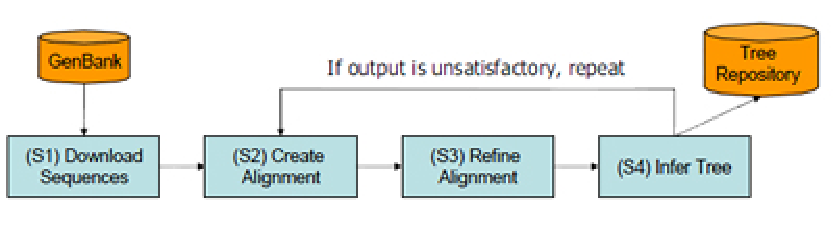
\includegraphics{./Figures/figure1.pdf}
		\rule{35em}{0.5pt}
	\caption[Scientific Workflow]{Scientific Workflow. [6]}
	\label{fig:scientificWorkflow}
\end{figure}


Provenance of data was regarded as an important aspect of the databases storing scientific data. The majority of such databases are usually views of some bigger databases that store raw experimental data. In particular, several scientific stores are populated by the result of queries made to other databases, and are manually updated by several other experts. This sort of databases are commonly known as curated databases [1:53], due to the number of people and/or systems involved in the data insertion and update process. Thus, we can come to recognize that keeping provenance information can help to a great extent to understand the origin of a piece of data, and particularly the process that led to that piece of data. Eventually, we will be able to determine the accuracy, integrity and trustworthiness of data [3].
In the scope of databases, there are two types of provenance that can be observed: "where-provenance", "why-provenance" [3:7]. The former identifies the tuples that were involved in the production of a query result; whereas the latter helps identify the original location a piece of information was copied from.

Consider the following example

\begin{figure}[htbp]
	\centering
		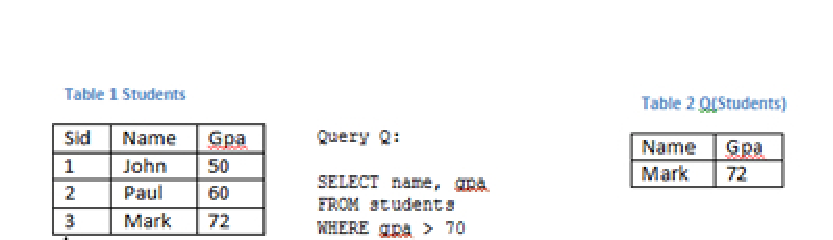
\includegraphics{./Figures/table.pdf}
		\rule{35em}{0.5pt}
	\label{fig:scientificWorkflow}
\end{figure}


Where-provenance can answer to a question such as, where the value gpa ' 72 in the tuple $(mark, 72)$ comes from. The answer would be, that it comes from the field gpa of the tuple with id = 3, in the students table.  Similarly, the why-provenance identifies that the tuple $(3, Mark, 72)$ was the one that contributed to the tuple $(Mark, 72)$ of the query result.
There is a third type of provenance which is called "how-provenance" [1:188]. While why provenance identifies the source tuples that justify a query result, how-provenance goes a step further and tries to describe how those tuples were involved in the creation of that result.

\subsection{Provenance Techniques}

In this section we present a classification of different methods that have been used to support data provenance. Figure 1.2 summarizes the five main aspects according to which we can classify the techniques for data provenance that have been proposed for use in individual domains. [4]

\begin{figure}[htbp]
	\centering
		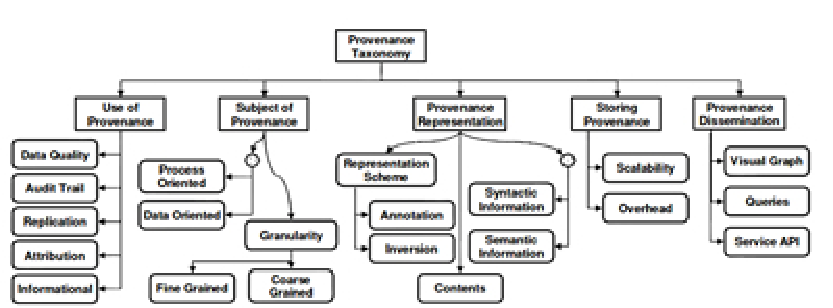
\includegraphics{./Figures/figure2.pdf}
		\rule{35em}{0.5pt}
	\caption[Taxonomy of Provenance]{Taxonomy of Provenance. [4]}
	\label{fig:provTaxonomy}
\end{figure}


\subsection{Applications of Provenance}

As we have already observed, provenance of data can be used for numerous reasons. A good summary the diversity of applications of data provenance is presented by Goble [4:14] and briefly described in the following lines:

\begin{description}
  \item[Data quality]
        Scientific databases and workflows, we examined earlier, belong to this category. Such systems sustain provenance information in order to help users reason about the quality, integrity and reliability of a piece of data.
  \item[Audit trail]
        Provenance can be considered as a logbook tracking all the steps (i.e. process execution details), resources (e.g. hardware, software, input data) and agents (e.g. users, external tools etc.) that were involved in the derivation of a piece of data or a computational result. This information can be useful twofold; locating possible reasons for the existence of an error and for determining resource usage. [4:8]
  \item[Replication recipes]
        Just as is the case in scientific workflows, keeping track of how a computational process was performed, can be useful for validating the results by repeating the same execution.
  \item[Attribution]
        Provenance can be used to tackle the problem of attribution which various systems (e.g. curated databases) usually suffer from [1:53]. More specifically, systems where different users can perform update actions to a dataset, provenance can help attribute the ownership and find the original creator of a piece of data.
  \item[Informational]
        Systems were data are the result of the execution of a sequence of complex tasks (e.g. scientific workflows), provenance is a mean for interpreting data-intensive analysis [6].
\end{description}

\subsection{Subject and Granularity of Provenance Information}

When designing a provenance-aware system, one should specify the subject of provenance - the provenance of what? -  as well as the level of information detail.

Yogesh, et al. [4] introduce two models of provenance: in a data-oriented model, the provenance of data is compiled explicitly in the form of metadata. For example, a directed acyclic graph (DAG)  [1:298] can explicitly present the provenance of a piece of data, by simply describing the process that led to its current state.  Contrary to that, the process oriented model suggests that the deriving processes are entities for which provenance is recorded.  Hence the data provenance is implicitly determined by examining the inputs and outputs of those processes.

The granularity refers to the smallest piece of information that provenance is tracked for. For example, in a relational database we can decide to track provenance to the level of rows or cells. Essentially, the system requirements need to determine the level of granularity.


\subsection{Provenance Representation}
There are two major approaches for computing data provenance [5]: (i) non-annotation (or inversion method) approach and (ii) annotation approach.

\begin{figure}[htbp]
	\centering
		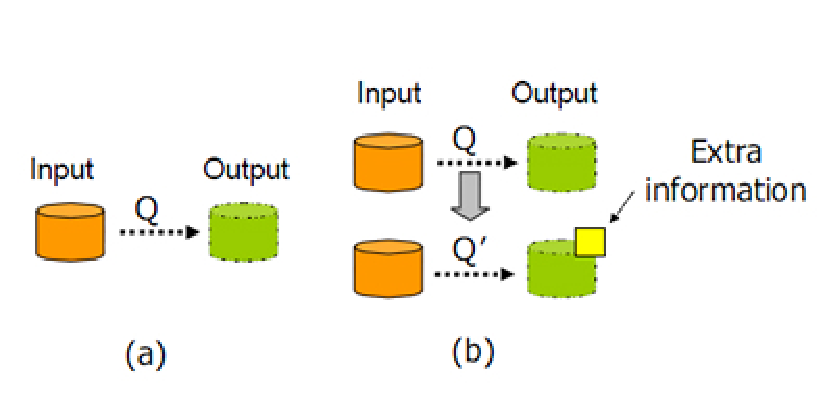
\includegraphics{./Figures/figure3.pdf}
		\rule{35em}{0.5pt}
	\caption[Provenance Represantation]{(a) Non-Annotation (NA) approach, (b) Annotation (A) approach. [5]}
	\label{fig:provRepresentation}
\end{figure}

Consider the example in figure 1.3a.  Q is the transformation function (i.e. query) that acts upon an input database with the aim to generate an output database. This is an example of a non-annotation approach whereby the provenance of the data product (i.e. output database) is computed by analyzing the input and output database, and the definition of Q (e.g. by analyzing the underlying algebraic structure of the query [6:18]). On the other hand, the annotation approach is slightly different. Provenance is determined by collating extra information in the form of annotations and descriptions about other resources. In this approach, provenance is serialized in a machine readable format (e.g. xml, rdf/xml).



\subsection{Provenance Dissemination}

Regardless the representation format of provenance, one should be able to view and act upon this captured information. A system needs to provide access and present provenance in both, a user and machine friendly manner. A common way is to visually represent provenance graphs. However, there is a significant caveat. Big provenance graphs are not intuitive and make it difficult for a user to interpret. Hence, this approach is not scalable. A better solution is to support a query engine which can extract smaller parts of a provenance graph.

\subsection{Provenance open data models}

In the previous section we examined how provenance systems have been integrated within scientific workflows and database management systems. Such systems, though, have full control of the information they process and store and thereby they track provenance within their own scope. Architecture like that, promotes tight coupling between the various systems components (e.g. provenance system, execution environment etc.) [8]

In the era of distributed systems, interoperability is a significant factor that needs to be considered. To that end, systems should adopt mechanisms and techniques that utilize open and technology agnostic models. Several approaches for promoting interoperability rely on an infrastructure that supports several provenance stores [8:55, 8:56] which offer long-term persistent storage of provenance information. Nevertheless, the representation of the provenance information should be described in a coherent way, regardless of the technologies involved.

The intent of this section is to summarize some early attempts for designing a common provenance model, as well as, the current W3C provenance data model (by the time of this writing, the W3C provenance working group1 has published a working draft of the specification)


\subsubsection{Provenance in Service Oriented Architecture (SOA)}

Service oriented architecture (SOA) is an architectural style that has been successfully used in distributed systems. The major advantage of a SOA based system is the loose coupling between the various software components, which minimizes the system development time, as well as, the maintenance cost. Applications following the SOA approach are mainly composed dynamically by utilizing services available in a network [SOA reference]. Thus, the need of a shared and technology-agnostic data model is critical for such systems to be able to manage provenance information.

One of the early attempts to integrate provenance systems into SOA applications was the PASOA approach [mash-ups]. According to the PASOA model, provenance information is described with the notion of proves assertions (p-assertions) [9]. P-assertions are, essentially, assertions made by individual services about their involvement in a process execution. Furthermore, they are the main constituents of a process documentation, which in order, provides with description about what happened at execution time (e.g. which algorithms, data sets or services were involved).

Something that is noteworthy at this point is that the full details of the process that brought a data item to its current state, can considerably huge (theoretically can trace back to the big bang [1]). For example, the full provenance of a result produced by a service that calculates the carbon footprints of individuals might include descriptions of the algorithms that were used, users' input, carbon emission calculation methods, data compiled by external devices (e.g. Gps) and so forth. However, this amount of information might be frustrating for a user who wants to obtain the provenance of a specific piece of data. This fact unveils the need of a query engine where users can provide with customized queries, so that they can get the information they need and avoid the information overload.

During a process execution, there are various tasks carried out. For example, different services might interact with each other by exchanging messages (e.g. SOAP messages) or a single service might apply different transformation functions to input data. As a result, the content of p-assertions can vary. We have three distinct categories of p-assertions based on the content of the provenance information that is being captured.

\begin{description}
  \item[Interaction p-assertions]
         It is an assertion that describes how data flows among the various services in a SOA system. An interaction p-assertion consists of an interaction key that identifies an interaction (i.e. source and destination services), as well as, the content of the message itself (e.g. content of SOAP message)
  \item[ Relationship p-assertions] 
      Assertions about how data slows throughout a single service. They can essentially, describe the function or algorithm that was applied to input data, in order to produce the output message.
       Example p19 from architecture for provenance

  \item[Service-state p-assertions]
        During a single execution, a service has a specific internal state. For example, information such as, CPU time used by a service, available space on the disk, user logged in, local time, might be useful to make various interpretations about the computational result.  P-assertions demonstrating all these information are called service-state p-assertions.
\end{description}

The aforementioned p-assertions describe the steps in the history of a process execution and can be visualized as directed acyclic graphs (see figure 1.4)

\begin{figure}[htbp]
	\centering
		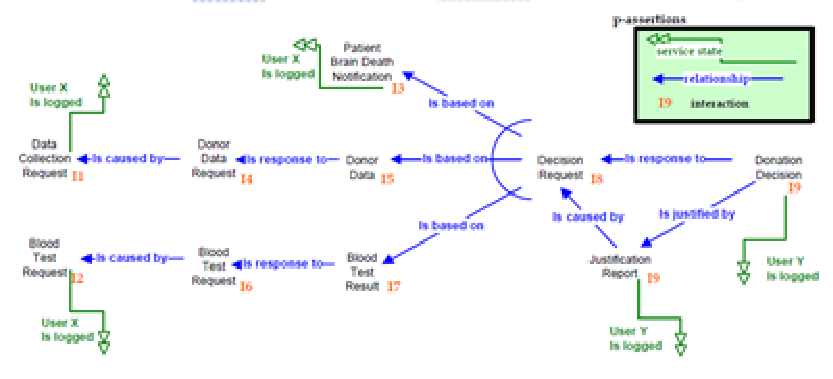
\includegraphics{./Figures/figure4.pdf}
		\rule{35em}{0.5pt}
	\caption[Provenance Directed Graph]{Provenance Directed Graph [9]}
	\label{fig:provGraph}
\end{figure}


\paragraph{Provenance life-cycle}

In this section we briefly describe the different phases that constitute p-assertions life cycle [10]. More specifically, p-assertions pass through four distinct phases, which we outline below.
\begin{enumerate}
  \item
        \textbf{Creating p-assertions:} As we have already mentioned, services are responsible for creating p-assertions while execution precedes each service can only describe its own involvement in the process execution.
  \item
        \textbf{Recording p-assertions:} A provenance store, as described earlier, offers a long-term persistent storage for p-assertions. Hence, after they are created, p-assertions have to be stored in a provenance store, for future use.
  \item
        \textbf{Querying p-assertion:} A provenance store offers a helpful mechanism for obtaining the provenance of a specific piece of data. More specifically, a user can compose queries that will bring the p-assertions according to the users need. In essence, the query will be executed over a process documentation that embraces all the p-assertions.
  \item
        \textbf{Managing p-assertions:} P-assertions may be stored in a provenance store for a long period of time. They therefore may need to be managed over the course of time.
\end{enumerate}

A complete provenance system has to support all these phases of the provenance life-cycle.

\paragraph{A Conceptual Provenance Architecture}

In the previous section we outlined the four main phases of the provenance (or p-assertion) life cycle. For a system to be able to support those phases, a logical architecture that will consist of appropriate system components, has to be designed. Groth et al. [10] suggest generic provenance system architecture (see figure 1.5).

\begin{figure}[htbp]
	\centering
		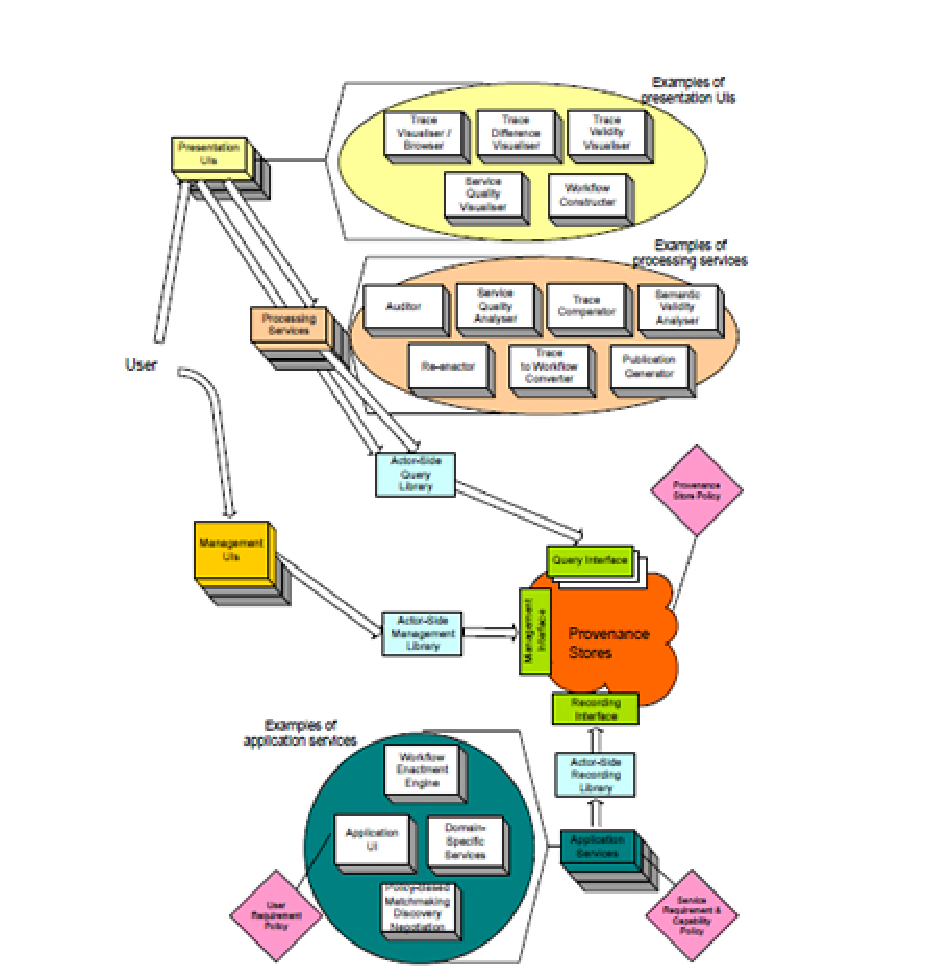
\includegraphics{./Figures/figure5.pdf}
		\rule{35em}{0.5pt}
	\caption[Architecture of Provenance-Aware Application]{Architecture of Provenance-Aware Application. [10]}
	\label{fig:provArch}
\end{figure}

In this architecture, we can observe four different actors that are involved in the provenance life-cycle

\begin{description}
  \item[Application actor] 
        It is the system component that processes the business logic of the application.
  \item[Provenance store] 
        This is the central point in the architecture. As we have already described, it is the responsibility of the provenance store to persist and provide access to the recorder provenance information.
  \item[Querying actor] 
        This is the part of the system that communicates with the provenance store by issuing provenance queries.
  \item[Recording actor] 
        While the querying actor send queries to the provenance store, the recording actor populates it by submitting p-assertions. 
  \item[Asserting actor] 
        This is the actor that creates appropriate p-assertions while the execution proceeds.
  \item[Managing actor] 
        An actor that performs all the managing tasks in the provenance store.
\end{description}

It is obvious that the provenance store is the key actor in the provenance lifecycle. It interacts with several other system components and therefore should provide appropriate interfaces to facilitate those interactions.

\begin{itemize}
  \item 
        A \emph{recording interface} which give access to recording actors so that they can submit p-assertions.
  \item 
        A \emph{query interface} which is the entry point for query actors so that they can issue provenance queries and get back the query results.
  \item 
        A \emph{management interface} which allows managing actors to perform managing tasks in the store.
\end{itemize}

    
\subsubsection{Open Provenance Model}
The provenance data model we presented earlier, describes a shared models for capturing, recording, exchanging and managing provenance information. However, it is primarily bound to SOA applications, that is, to message exchanging systems. The models that we discuss in this section is the first purely technology agnostic provenance data model.

The Open Provenance Model (OPM) [1:299] addresses different provenance interoperability issues by introducing the notion of the provenance interoperability layer [1].

Figure 1.6 illustrates a big system which consists of several individual applications. Each of these applications is designed to be provenance aware and makes use of its own provenance store. In a system like that, where information flows across different applications, the history of the derivation of a piece of data (i.e. provenance) might reside across several provenance stores. As a result, one would need to query several provenance stores, to form the whole process execution chain. It is the job of the inter-operability layer to conceal the technology diversity of individual applications and expose provenance data in a uniform manner.

\begin{figure}[htbp]
	\centering
		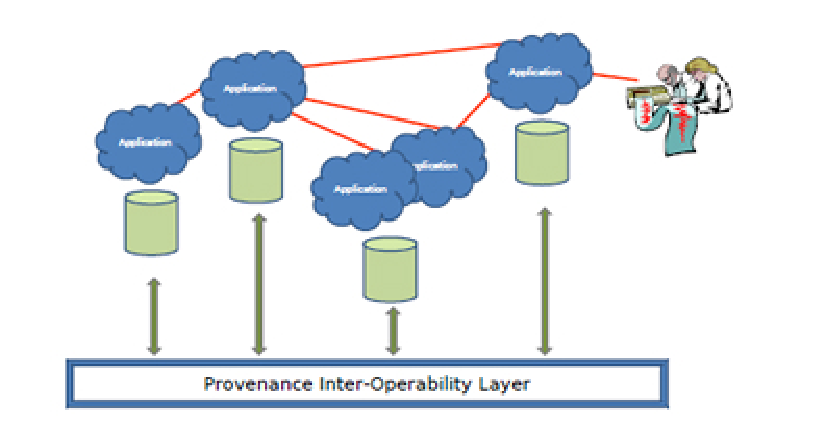
\includegraphics{./Figures/figure6.pdf}
		\rule{35em}{0.5pt}
	\caption[Cross-System Provenance]{Cross-System Provenance. [1]}
	\label{fig:provAccrossSystems}
\end{figure}

The open provenance model utilizes a graph structure to represent a set of causal dependencies [13] among its nodes. A set of such dependencies can explain how a digital piece of data, physical resource (e.g. bicycle) or a conceptual entity (e.g. immaterial entity, idea etc.) came to be in a particular stat at a specified time.

OPM suggests three types of nodes, which we now present:

\begin{description}
  \item[Artifact] 
         A digital, physical or conceptual entity can have different sets of characteristics, at different moments. We call this specific state of an entity, an artifact. An artifact can be viewed as a snapshot of an entity at a given moment. For example, a pdf file at a specific time. States are immutable in that they cannot be modified. Alterations to any characteristic of an entity at a given time result in the generation of a new artifact.
  \item[Process] 
        A process refers to an action or a sequence of actions that result in the generation of new artifacts. For example the process of embedding images into a pdf file produces a new pdf file, enriched with multimedia characteristics (i.e. images).
  \item[Agent] 
        Agent is an entity which triggers a process. in other words, it is the responsibility of an agent to initiate or terminate a process. Following the example with the pdf file, an agent might be a software component that initiated the process of adding images into the new file.
\end{description}

Nodes in an OPM graphs are connected with each other via causal dependencies. Such dependencies are illustrated with directed edges from the source bode (or effect) to the destination node (or cause).

The OPM model introduces an initial set of causal dependencies which are illustrated in figure 1.7. This is a graphical representation of the causal relationships between artifacts, processes and agents. Artifacts are represented by ellipses; processes are represented by rectangles; and agents by octagons. [OPM v1.01]

\begin{figure}[htbp]
	\centering
		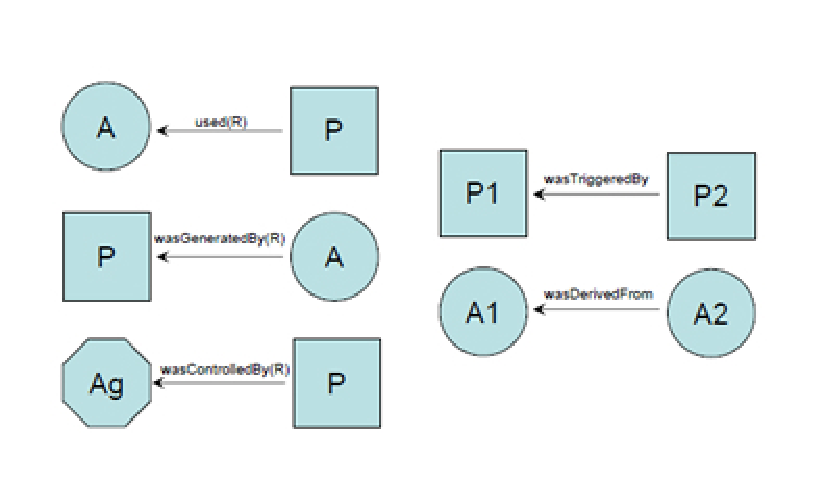
\includegraphics{./Figures/figure7.pdf}
		\rule{35em}{0.5pt}
	\caption[Provenance Causal Dependencies]{Provenance Causal Dependencies [13]. Note that past tense aligns with the notion of process history documentation.}
	\label{fig:provCausalDependencies}
\end{figure}

We observe a set of five types of causal dependencies based on participants.

\begin{description}
  \item[Used] 
        A relationship between a process and an artifact denoting that the process used the artifact to produce a result (e.g. a new artifact). The formal definition suggests that the availability of the artifact is critical for the process to complete the execution.
  \item[wasGenerateBy] 
        It is a relationship between an artifact and a process, indicating that the artifact was generated by the process. In other words, the existence if the artifact is due to the execution of that process.
  \item[wasTriggeredBy] 
        Figure 1.7 shows an edge wasTriggeredBy from a process p2 to a process p1. The semantics of this relationship defines that there was some unknown artifact that was generated by some process p1 and was used by a process p2.
  \item[wasDerivedFrom] 
        An edge wasDerivedFrom from an artifact node A2 to another artifact node A1 denoted that there was a process that used tan artifact A1 to generate an artifact A2. It is a useful relationship, when the actual process of a transformation is unknown.
  \item[wasControlledBy] 
        It is a causal dependency between a process and an agent. It simply indicates that the execution (i.e. the start and end) of a process is carried out under the control of an agent.
\end{description}

Note the letter R in the "used", was controlled by" and "was generated by" edges. This is a bit of extra information that is used in the aforementioned relationships to characterize the role of each entity (i.e. artifacts, agents) that is connected to the same process. More specifically, in a "used" relationship, the same process may use several artifacts. However, the nature of each usage might be different. For instance, an online process for searching for news based on a keyword and a specified source uses the keyword with the role "keyword to search" and the source web site with the role "web site to search". Similarly, a process can generate several artifacts with different role each. Following the previous example, the process can produce a news article and a set of additional sources. The former will have the role "article associated with the keyword" whereas the latter will have the role "additional sources to look at". Finally, a process can be controlled by multiple agents, each with a distinct role. In the example of the online news fetcher, the process for searching news can be initiated either by a user via a user interface, or by an external application via an application programming interface (API). The Roles in this case might be "internal actor" and "external actor" respectively.

One of the concepts associated with provenance that we have been constantly highlighting, is the ability to specify the scope of the provenance that is being captured.  A provenance of a piece of data can be expressed in various levels of detail. Furthermore, it can be viewed from different angles and standpoints. To that end, OPM introduces the notion of accounts [13]. An account is regarded as a graph coloring, indicating different provenance sub-graphs which provide details at different level of abstraction.

P6 figure 10 with accounts

The concept of accounts is fairly useful and caters users with multiple descriptions of the provenance of the same piece of data.
A final note about OPM concerns the extensibility capabilities of the model. Stronger interpretations of the causal dependencies we described in this section can be used to serve application-specific requirements. A common way to achieve that would be to design an ontology with subclasses of those causal dependencies.


\subsubsection{The W3C Provenance Working Group}
The open provenance model was a good initiative to tackle with inter-operability issues pertaining to the provenance dissemination across multiple platforms. However, as is the case of many widely used technologies, there should be a consensus among different bodies (e.g. industry, academia etc.) about the final specification. For this reason, the provenance working group was formed in the World Wide Consortium (W3C). The group followed the work that was started by the Provenance Incubator Group\footnote{$http://www.w3.org/2005/Incubator/prov/wiki/W3C_Provenance_Incubator_Group_Wiki$}. The ultimate goal of the group is to reach an agreement upon the specification of provenance on the World Wide Web.

At the time of this writing, the provenance working group has published a set of specifications which are still on the "working draft" step of the W3C specification approval process. In particular, the specifications that have already been released are:

\begin{description}
  \item[PROV Data Model] 
        A data model for describing all the parties that are involved in the generation of a data item [15].
  \item[PROV Ontology] 
        A OWL 2 web ontology for expressing the PROV data model. In essence, it is the "vocabulary" that is used by the PROV data model to represent provenance information [?].
  \item[PROV Notation] 
        Specification which aims to design the means for a human friendly representation of the information expressed by the Prov data model[?].
  \item[PROV Constraints] 
         A document that defines a set of constraints that assures the validity of PROV instances (statements). Further, it specifies inference rules for reasoning over PROV instances. This can result in the creation of additional statements implied from the explicitly stated provenance information[?].
  \item[PROV Access and Query ] 
        A document that describes the means to leverage the existing web infrastructure, in order to query and obtain provenance information[?].
\end{description}

In this section, we will present the PROV data model (PROV-DM). For additional information about the rest specifications, we refer the reader to the official web site  of the W3C provenance working group\footnote{$http://www.w3.org/2011/prov/wiki/Main_Page$}


\paragraph{PROV Data Model}
Provenance can be viewed from different standpoints, and therefore various kinds of information can be stored in provenance records [14].

The provenance data model identifies three distinct perspectives of provenance:

\begin{itemize}
  \item 
        \textbf{Agent-centered provenance:} emphasis is given on the entities that took part in the generation or manipulation of the data item in question. For example, considering the provenance of a video file in a blog post, we might want to know the person who recorded that video, the person who edited it, and the user who posted it on the blog.
  \item 
        \textbf{Object-oriented provenance:} a different perspective suggests that we might want to identify the origin of different parts of a document. For example, in the same blog post, we may want to know that the video was taken from YouTube and the images from Flickr.
  \item \textbf{Process-oriented provenance:} finally, we may want to highlight the actions that were carried out to generate a data item. For example, a visual graph illustrating the connections I have in a social network site may have been generated by invoking a service to pull data from the social network, which then are processed by a JavaScript library for visualization.
\end{itemize}

Regardless the various viewpoints that provenance can be examined, a good data model should provide all the means needed to capture adequate information. To that end, the PROV-DM introduces some key concepts, which we outline in the following lines.

\begin{figure}[htbp]
	\centering
		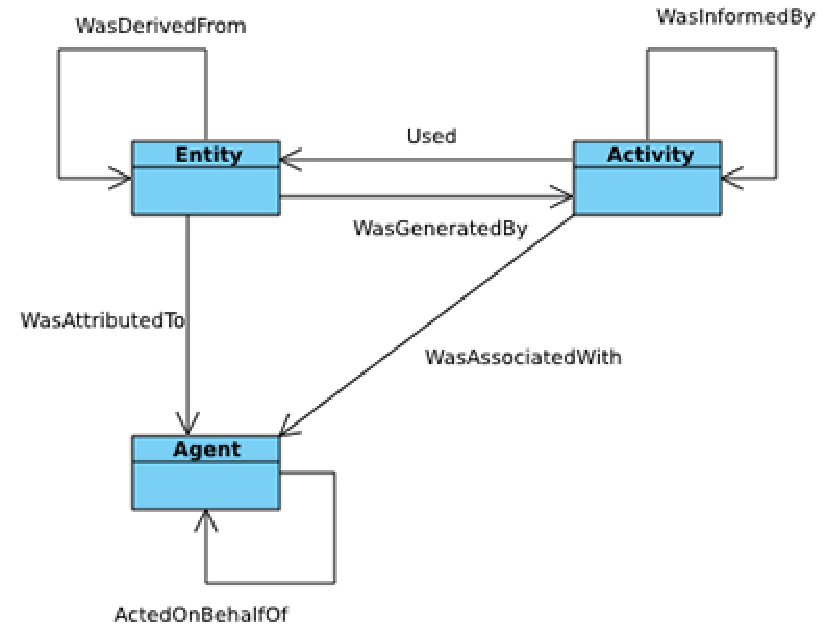
\includegraphics{./Figures/figure8.pdf}
		\rule{35em}{0.5pt}
	\caption[PROV-DM]{PROV-DM [14]. Note that past tense aligns with the notion of process history documentation.}
	\label{fig:provDM}
\end{figure}

An entity is the equivalent to an artifact in the open provenance model. It may refer to a physical, digital or immaterial thing, such as a blog post, a car or a decision. The second, constituent is the activity. This is equivalent to a process in OPM model and represents the derivation of an entity. In particular, it refers to process of generating a new entity or the transformation of one entity to another. For example, the process of calculating the carbon emissions of an individual based on some input data is an activity. Finally, an agent in PROV-DM is assigned a degree of responsibility for an activity that is being carried out. The concept of an agent is similar to that of an actor in the OPM model, in that represents a "thing" that is responsible for controlling the execution of an activity. An agent can be a human being, an organization, software or any other entity that may initiate an activity. For example, a JavaScript visualization library can be an agent that is responsible for imitating a graph visualization activity.

At this point we have to note that provenance can be expressed only for entities. However, we can make provenance assertions about an agent, should the agent be declared both as an agent and an entity.
These are the main concepts of the PROV-DM data model. In addition to that, the data model encompasses several other relationships (for additional information, refer to the official document [15]).


\paragraph{Entity Generation and Usage}

An activity in PROV-DM can be related to an entity in two different ways.  First of all, the effect of the actions that comprise an activity is usually the generation of new entities. Hence, entities exist due to activities existence. For example, assembling car parts brings a car into existence. Additionally, activities can use entities, often during the process of generating other entities. For example, a visualization activity can use some datasets stored in a database, in order to create a chart. These two relationships are represented in the PROV-DM with the terms \emph{wasGeneratedBy} and used respectively

\paragraph{Agents' Responsibility}

Agents can be associated with entities, activities or other agents. Relationships between entities and activities come in the form of responsibility that an agent has over them. We have already highlighted that agents are responsible for the execution of an activity. A responsibility might refer to an agent initiating or terminating an activity. For example, in PROV-DM we say that an activity was associated with an agent. Similarly, an activity can be responsible for an entity. This form of responsibility can be interpreted as the attribution of an entity to an agent. In other words, the was AttributedTo relation, from an entity to an agent, denotes that an agent was responsible for an activity that was the cause for this entity to be created. This is useful relation when the activity is unknown or of a little significance. Finally, PROV-DM provides mechanisms to express relations between two agents. In particular we say that an agent can act on other agent's behalf.  For example, an employee can be designated by the company to perform some actions on their behalf.

\paragraph{Entity Derivation}

The last core relationship defined by the PROV-DM is a relation between two entities. The existence of an entity might often be due to some other entity that was used by the activity that generated it. In that case, it is said that one entity was derived from another entity. A special kind of such relation is the "was revision of". For example, the PROV-DM specification may go through multiple revisions over the course of time. Such relation can be useful to examine the changes that had been brought across the different revisions of a document.

\paragraph{Roles}

Recall the notion of roles in the OPM model. The PROV-DM has adopted the same notion to characterize relationships between entities and activities. In particular, a role specifies how an entity was used or generated by an activity. Similarly, roles can specify the nature of agents' involvement in an activity. It is obvious that roles are application specific, and therefore are not specified by PROV-DM.

\paragraph{Plans and Accounts}

Activities may consist of numerous steps and procedures. For instance, an online tutorial for publishing links data on the web illustrates several steps that should be taken. In PROV-DM there is a specific term to represent this set of actions. In PROV-DM language, this term is called plan. Plans are entities, therefore we can describe provenance for them.
Finally, one would wonder how we can trust the provenance information about a resource. In fact, this is a plausible question, since anyone can make provenance assertions about any entity. The PROV-DM supports a means to address this issue, namely it includes the notion of accounts. In essence, an account is an entity that contains some provenance information, and because it is an entity, we can express a provenance for it. That is to say, provenance of provenance can be expressed.

Example [15]
\begin{verbatim}
Entity(ex:w3c-publication.pn, [prov:type="prov:Account" % % xsd:QName])
wasAttributedTo(ex:w3c-publication.pn, w3:consortium.)
\end{verbatim}

In the above example, which was written in PROV-Notation, we have explicitly declared the "ex:w3c:publication.pn" provenance description. We then state that "w3:consortium" agent was responsible for its generation.

In this section we presented only the core principle of the PROV-DM specification. However, the whole specification is very rich and consists of many more concepts and definitions. For this reason, we would recommend the reader to visit the provenance working group web site to read the whole set of PROV specifications.

\subsection{Security}

A provenance -aware system is, essentially, capable of recording and storing provenance information about different assets that reside in system. As we have already discussed, this sort of functionality is accomplished with the aid of a data model, which defined the way that provenance information is represented internally. Further, the presence of a provenance store guarantees the long-term storage of provenance information, as well as, provides a means for querying the store [19:5]. The result of a provenance query is a causal graph or provenance graph, which illustrated the provenance information in a way that can be viewed an analyzed.

Throughout the process described above, there is nothing that guarantees the quality and integrity of provenance information. To address this problem a framework that will consider all the security-related aspects of the provenance information, have to be devised. Such framework can leverage existing technologies (e.g. cryptography), that have been successfully applied on the web.
We will start our discussion by introducing some fundamental concepts and technologies pertaining to the security in computer systems.

\subsubsection{Fundamental concepts}

A discussion about security issues concerning the communication between different entities, which exchange some sort of information, should start by defining some initial security requirements. More specifically, there are five requirements that a secure system must provide.

\begin{description}
  \item[Confidentiality] 
        A system has to guarantee that all the information that is being exchanged between different entities is protected against eavesdroppers; for example, the information that we exchange when purchasing a product on eBay, should not be wire tapped by anyone.
  \item[Integrity] 
        A message sent from one to entity to other should not be altered, whatsoever; foe instance an order sent to eBay has to remain intact while traveling through the wire.
  \item[Authentication] 
        A mechanism that blocks unauthorized users from accessing the systems data and functionality. Access should be granted only to those users who can provide adequate information, in order to prove their identity; for instance In order to be able to perform a purchase action on eBay, one should provide his credentials.
  \item[Non-repudiation] 
        An important requirement in the communication between two entities is to be able to prove that a message was indeed sent by its sender; for example, once a user submits a purchase order, she cannot claim that has not done so.
  \item[Authorization] 
        This requirement is also known as access control. It, essentially, is a mechanism that determines the sort of access that a user can have on systems resources; for example, as an ordinary user, I cannot modify the systems database by deleting items that I am not authorized to delete.
\end{description}

\subsubsection{Cryptography}

Authorization and authentication are two requirements that can be achieved fairly easier that the rest. To support authorization, a system can simply apply one of the proposed models for access control (e.g. MAC [?], DAG [?], RBAC [?], ABAC [?] etc.). Similarly, authentication can be achieved by leveraging the current web infrastructure and the HTTP protocol capabilities (e.g. content negotiation). To meet the rest requirements, a system can use cryptography technics. More specifically, confidentiality can be ensured with encryption [?] whereas non-repudiation with digital signatures [?]. Finally, integrity can be guaranteed with either of those two technics. We review those technologies in the following sub-sections.

\paragraph{Symmetric Encryption}

This type of encryption requires that the entities that participate in a message exchange communication use the same key for the encryption and decryption phase. For example, figure 1.9 illustrates a message exchange scenario.

\begin{figure}[htbp]
	\centering
		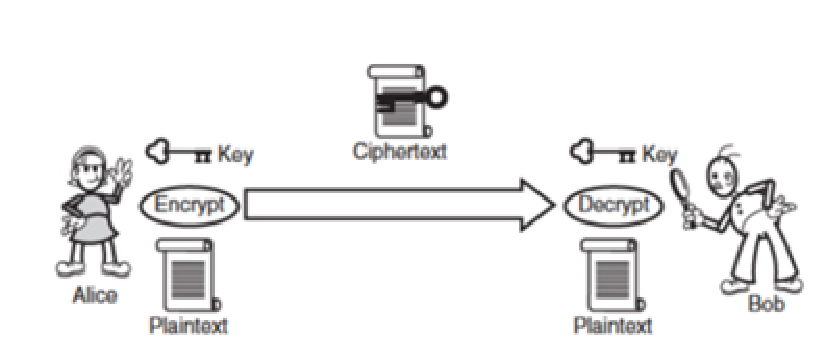
\includegraphics{./Figures/figure12.pdf}
		\rule{35em}{0.5pt}
	\caption[Symmetric Encryption]{Symmetric encryption. [?]}
	\label{fig:symmetricEncryption}
\end{figure}

In this scenario Alice wants to send a message to Bob. As shown in the figure, she encrypts the original data (plaintext) with a private key, and sends it to Bob who decrypts the encrypted message (cipher text) using the same private key. Some of the algorithms that can used to encrypt data are: 3DES, DES, AES, RC4

\paragraph{Asymmetric Encryption}

Asymmetric encryption is more flexible, in that two different keys are used: a private and a public key; for example, figure 1.10 demonstrate the same scenario but now an asymmetric encryption is used. Alice uses Bob's public key to encrypt the plaintext and sends it to Bob, who decrypts the cipher text using his private key.

\begin{figure}[htbp]
	\centering
		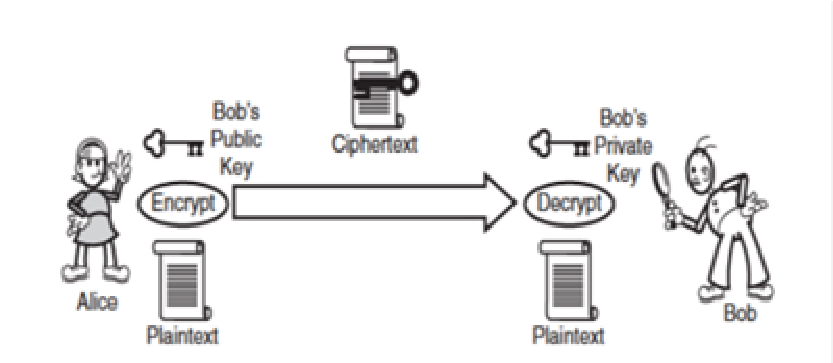
\includegraphics{./Figures/figure13.pdf}
		\rule{35em}{0.5pt}
	\caption[Asymmetric Encryption]{Asymmetric encryption. [?]}
	\label{fig:asymmetricEncryption}
\end{figure}

\paragraph{Digital Signature}

Integrity and non-repudiation can be guaranteed with the use of digital signatures. To better describe this technology look at figure 1.11. Alice has a pair of private and public keys.

\begin{figure}[htbp]
	\centering
		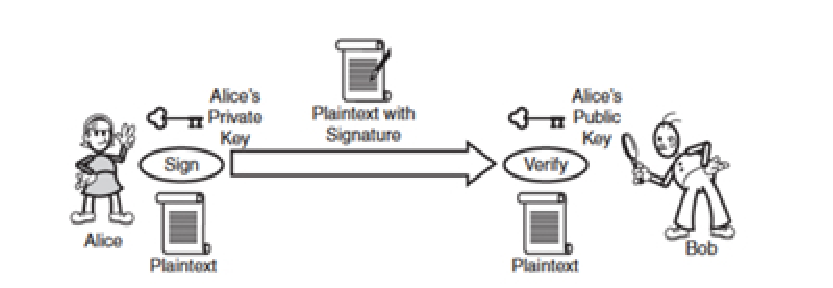
\includegraphics{./Figures/figure14.pdf}
		\rule{35em}{0.5pt}
	\caption[Digital Signature]{Digital Signature. [?]}
	\label{fig:digitalSignature}
\end{figure}

She creates a signature value with her private key and sends it to along with the original plaintext. On the other side, Bob uses Alice's public key to generate a signature value based on the content of the message he received. He then can compare the two signatures to verify the integrity if the incoming message.

\paragraph{Asymmetric versus Symmetric Encryption}

A noticeable caveat of the symmetric encryption is the key distribution problem. Both participants need the same key to encrypt and decrypt a message; therefore they need to somehow exchange it. This has to be done carefully to avoid malicious attackers from stealing the transmitted keys. On the other hand, the most evident downside of the asymmetric encryption is that it exhibits very poor performance. Asymmetric encryption is much slower that symmetric.

\subsubsection{Security protocols}

SSL is probably the most prevalent security protocol for distributing keys in a safe mode. It, essentially, defines the requirements for a secure exchange of keys between two parties. The main steps described by the protocol are the followings:

\begin{enumerate}
  \item 
        The client communicates with a server
  \item 
        The server responds back by returning its certificate
  \item 
        The client computes a random number which represents a seed for generating private keys. He then encrypts this number using the public key included in the server's certificate and sends it to the server.
  \item 
        The server obtains the random number by decrypting the received message
  \item 
        Ultimately, both parties have the same seed; they therefore can create the same private key.
\end{enumerate}

\subsubsection{Public key infrastructure}

As described earlier, in the asymmetric encryption we do not need to bother about how to distribute private keys, since we can share a public key. However, it is critical that we associate the public key with a particular party. In other words, the owner of the public key has to be identified. To that end, the Public Key Infrastructure (PKI) has been designed. The main constituents of PKI are: a certificate, which is a digital resource that associates a participant to a public key. This certificate is digitally signed and issued by a trustworthy third-party authority, which is called Certificate Authority (CA). There is a relatively small number of CAs in PKI and they can issue certificates to other certificate authorities.

To better describe this infrastructure, consider the following example. Figure 1.12 illustrates a typical PKI scenario.

\begin{figure}[htbp]
	\centering
		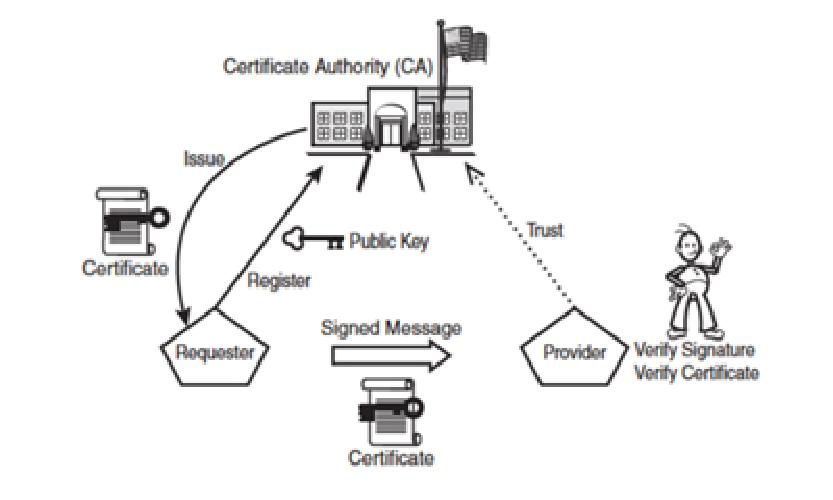
\includegraphics{./Figures/figure15.pdf}
		\rule{35em}{0.5pt}
	\caption[Public Key Infrastructure]{Using certificate for a digital signature. [?]}
	\label{fig:pki}
\end{figure}

Alice signs a message with a private key and sends it to Bob along with a certificate.  Bob creates a signature value using the public key contained in the certificate. But before that, he has to verify that the certificate is signed by a trustworthy certificate authority.

\subsection{Publishing and querying provenance information}

An important task for a provenance-aware system is to capture and store provenance information. An equally crucial feature is to be able for someone to locate that information and ultimately query and retrieve it some format.  For that reason, an infrastructure should be supported so that external applications, users or the application itself could reuse the captured provenance information. Such infrastructure should resolve the problem of locating, retrieving and querying that information. The most appropriate solution is to leverage the current web infrastructure, as well as, some semantic web technologies. In more detail, uniform resource identifiers (URIs) can be assigned to provenance information (provenance-URIs), as well, as, its constituents (i.e. entities, activities and agents). Any application can then perform HTTP GET requests to access the information that is associated with the Uri in question [22]. This is similar to the way URIs are dereferenced when accessing web resources. Nevertheless, it not a strict requirement to assign unique URIs, due to the difficulties that such process has. Thus, alternative methods can be provided to facilitate the same functionality (we discuss them further in this section).

Locating provenance information is crucial and is indispensable in scenarios where a provenance-URI is unknown. In such occasions, an application or a user has to provide some additional information to a provenance provider, which can be a third-party application. According to the submitted information, a provider can locate the provenance-URI and/or the provenance information itself.

Provenance information, as already mentioned, consists of causal relationships between entities, activities, and agents. As such, it is a requirement that one can retrieve descriptions about those resources. The concept is similar, URIs (entity-URIs) can be assigned to those resources and one of the following mechanisms can be provided:

\begin{itemize}
  \item 
        In the case where the requester knows the entity-URI, a simple HTTP mechanism can be used to access the dereferenced content. More specifically, if a resource is accessible via an HTTP GET request, an additional link header denoting the URI where provenance for that resource is located can be injected into the header of the response.
        
\begin{verbatim}
Link: provenance-URI; rel="provenance"; anchor="entity-uri"
\end{verbatim}
        
        The \emph{entity-URI} indicates the location where additional description for that resource can be obtained, whereas the provenance-URI identifies the location of the provenance information which the entity is part of. If the provider though, does not know anything about provenance locations, it can point to a third-party provider or a provenance service. In that case, the link header is slightly different.
        
\begin{verbatim}
Link: provenance-service-URI; rel="provenance-service"; 
anchor="entity-uri"
\end{verbatim}
        
        The \emph{provenance-service-URI} will, essentially, return a service description that will aid a client to locate a provenance-URI or fetch provenance information for the entity in question.
        
  \item 
        For resources that are presented in HTML, provenance-URI can be included within the document. The simplest way to do that would be to use the <Link> html element. Consider the following example.
        
\begin{verbatim}
<html xmlns="http://www.w3.org/1999/xhtml">
    <head>
        <link rel="provenance" href="provenance-URI">
        <link rel="anchor" href="target-URI">
        <title>Welcome to example.com</title>
    </head>
    <body>
       ...
    </body>
</html>
\end{verbatim}
        
        Just as is the case with the previous approach, the document provider can point to a provenance service where the information is stored. In that case the HTML snippet will resemble the following one:
        
\begin{verbatim}
<html xmlns="http://www.w3.org/1999/xhtml">
    <head>
        <link rel="provenance-service" href="service-URI">
        <link rel="anchor" href="target-URI">
        <title>Welcome to example.com</title>
    </head>
    <body>
        ...
    </body>
</html>
\end{verbatim}
  \item 
        Finally, if a resource is represented in one of the several RDF serialization formats (i.e. RDFa, XML/RDF, N-Triples, Turtle etc.) then additional RDF triples can be inserted to describe the provenance of the resource. For this reason, the property \emph{prov:hasProvenance} is defined. The object for that predicate is the resource that contains provenance information about a resource that is subject of this triple.
        
\begin{verbatim}
@prefix prov: <http://www.w3.org/ns/prov#>
<> dcterms:title      "Welcome to example.com" ;
prov:hasAnchor     <http://example.com/data/resource.rdf> ;
prov:hasProvenance <http://example.com/provenance/resource.rdf> ;
prov:hasProvenanceService <http://example.com/provenance-service/> .
  :
(RDF data)
\end{verbatim}

\end{itemize}

\subsubsection{Provenance Services}

There might be occasions where the provenance-URI is unknown. In such cases, a provenance service can provide a means for discovering and/or retrieving provenance information. A provenance service might be supported by a third-party provider, and is uniquely identified via a service-URI. Dereferencing, this URI will bring a service description, which provides guidelines to clients about how to locate or/and fetch provenance information. Two mechanisms are supported to accomplish that task: the provenance discovery service mechanism gets the URI for some resource and returns a set (one or more) of URIs, pointing to the location where the provenance information can be acquired. Conversely, the provenance retrieval service is used when there is no URI associated with the provenance information. As such, the service is responsible for locating and retrieving that information, on client's behalf.

Details about these services are described in the service description, which should be in available as RDF (see example below).

\begin{verbatim}
<service-URI> a prov:ProvenanceService ;
    prov:provenanceUriTemplate "service-URI?target={+uri}" .
\end{verbatim}

The object of the \emph{prov:provenanceUriTemplate} is a literal values that contains a URI template\footnote{J. Gregorio; R. Fielding; M. Hadley; M. Nottingham; D. Orchard. URI Template. March 2012, Internet RFC 6570. URL: http://tools.ietf.org/html/rfc6570}. Users can replace the variable uri with actual uri of the entity for which provenance is required.

An alternative option is to use a query engine. For interoperability's sake, it is preferred that a SPARQL endpoint is used. Requesters can use a simple SPARQL query including an entity-uri, to get the corresponding provenance-uri.

\begin{verbatim}
@prefix prov: http://www.w3c.org/ns/prov#

SELECT ?provenance_uri WHERE
{
  <http://example.org/resource> prov:hasProvenance ?provenance_uri
}

\end{verbatim}

If the requester does not hold any URI, but knows some details about the resource, then those details can be included in the SPARQL query; for example if the DOI identifier for a document is known, then the following query can be submitted to the SPARQL  endpoint:

\begin{verbatim}
@prefix prov: http://www.w3c.org/ns/prov#

@prefix prism: <http://prismstandard.org/namespaces/basic/2.0/>
SELECT ?provenance_uri WHERE
{
  [ prism:doi "1234.5678" ] prov:hasProvenance ?provenance_uri
}
\end{verbatim}

Finally, if specific elements of provenance information are required, then the SPARQL query may look like the following:

\begin{verbatim}
@prefix prov: <http://www.w3c.org/ns/prov#>
SELECT ?generationStartTime WHERE {
    <http://example.org/resource> prov:wasGeneratedBy ?activity .
    ?activity prov:startedAtTime ?generationStartTime .
}

\end{verbatim}

In this example, the client wants to retrieve the start time of an activity in the provenance information in question.

\subsection{Carbon Footprints}

During the last century, human activities brought severe damages to the environment. This has been more evident during the recent years, where anthropogenic environmental impacts have led to severe climate changes [23:1]. To that end, several mechanisms to tackle with this problem need to be devised. In this section we introduce the fundamental terms and concepts that underpin the process of quantifying human's impact on the environment.

\subsubsection{Fundamental Notions}

Carbon footprinting is probably the most prevalent method for quantifying human's impact on the environment. More specifically, the term "footprint" can be associated with quantities of \emph{Greenhouse Gas (GHG)} emissions [Daniel Lashof] caused by activities, individuals, systems or populations. In cases where a more accurate evaluation of climate risk is needed, a measure called \emph{climate footprint} [23:3] can be used. Figure 1.13 illustrates the distinction of those measured. We can notice a third layer which corresponds to a yet broader set of GHGs emissions and is called \emph{GHG inventory}.

\begin{figure}[htbp]
	\centering
		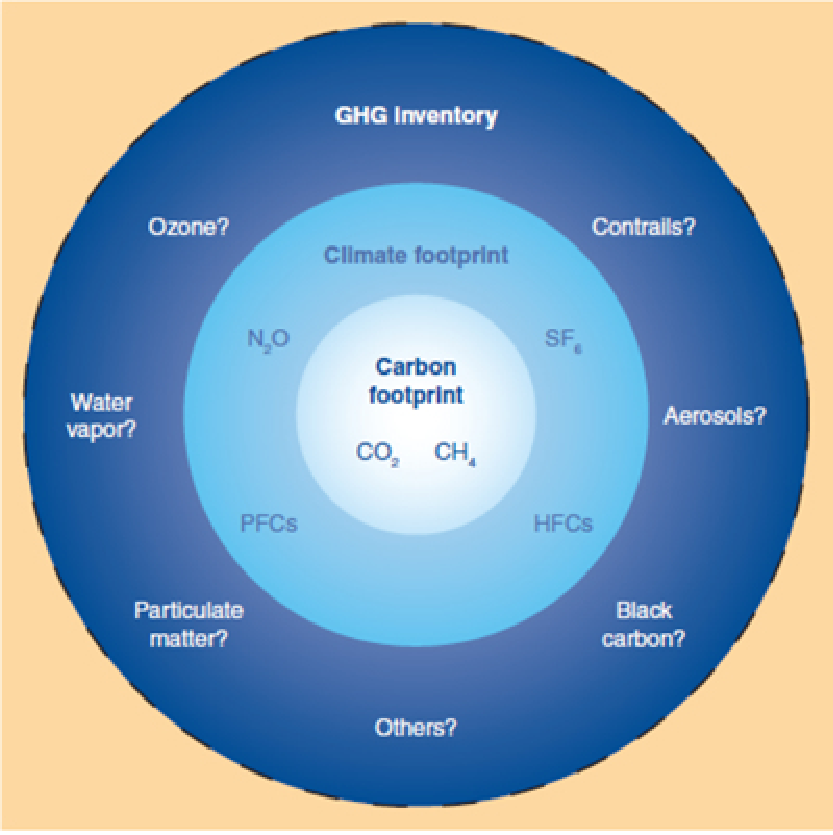
\includegraphics{./Figures/figure16.pdf}
		\rule{35em}{0.5pt}
	\caption[Carbon Emissions Measures]{Three measures for carbon emissions [23]}
	\label{fig:ghgEmissionMeasures}
\end{figure}

\subsubsection{Calculating carbon emissions}

The process of calculating carbon footprints is relatively straightforward and consists of the several steps.

\begin{enumerate}
  \item 
        Initially, all emission sources for the subject need to be compiled and classified; for example, an emission source for an individual might be his daily travels to work with bus.
  \item 
        A method for quantifying the emissions of each source has to be selected. The unit for that quantity is expressed in CO2e, which combines CO2 and CO4 emissions.
  \item 
        All the data that are needed by the method have to be gathered; for example, a method might need some activity data [25] and an appropriate conversion factor (or emission factor); we will come back to these terms in a bit.
  \item 
        A documentation of the method is vital, so that computed values can be validated by re-executing the same method, in the future. Provenance, which we discussed in previous sections, can be a good solution.
\end{enumerate}


\subsubsection{Gathering Emissions Sources}

The carbon footprint calculation process starts by gathering the emissions sources for the subject. To better identify possible emissions sources we can distinguish two types of emissions: direct and indirect emissions.

Direct are the emissions which the subject has full control of. These are the emissions that are primarily produced during the combustion of fossil fuels. On the other hand, indirect emissions are not directly associated with a specific activity, but are due to the demand for products brought by the subject in question; for example, each product that we buy consists of a number of activities that result in the product being on super-markets shelves. Apparently, all these activities cause CO2e emissions. This implies that our demand for products indirectly produced a quantity of CO2e that was emitted to the environment.

\subsubsection{Classifying Emissions}
The prime reason that lies behind the decision for categorizing emissions is the problem of double counting. In essence, it refers to the problem of associating the same quantity of carbon emissions to multiple subjects [23:25]. To avoid this issue, emissions are classified into three distinct scopes.

\begin{description}
  \item[Scope 1]
        In scope 1, the direct carbon emissions of individuals, activities or systems can be found; for example, carbon emissions produced by a car owned by a company.
  \item[Scope 2] 
        Scope 2 consists of emissions that are produced from energy generation. It basically, refers to energy purchased by the subject in question, for own consumption.
  \item[Scope 3] 
        Emissions which are the result of the subject's actions that take place outside the organization or geographic boundaries are scope 3 emissions. In general, this sort of emissions are said to be shared by several subjects rather solely belong to one.
\end{description}


\subsubsection{Calculation Methods}

The next step in calculating emissions is to select an appropriate calculation method, based on the data that are available. The simplest formula suggests that the number of units of the activity that occurred be multiplied by an appropriate conversion factor (emission factor) [23:2]. To better illustrate this concept, imagine that the carbon emissions of a trip made by car needs to be calculated. In that case, we can multiply the distance travelled (or fuel consumed) by a value that define the CO2e emissions of that car per kilometer units.

According to the accuracy and quality of the data that are present, calculation methods can be classified into three categories or tiers; if we choose to use the fuel consumed by a car then several factors that determine the quality of this figure should be considered. The type of the journey, the vehicles age and condition are some of the factors that affect the quantity of fuel consumption. A tier Three method will consider all those factors, as it will use the actual quantity of the fuel used. Further, it will multiply this number by an emission factor published by a government body and which is associated with the particular fuel type. A tier Two method will be less accurate. It will take the distance travelled as the main activity data and multiply it by the emissions factor for the specific car model. Finally, a tier One method will yield the least accurate figure, because it will use the least specific data. In particular, an average distance (published by some government's authority) for that sort of cars will be multiplied by the emission factor associated with that fuel type.

\subsubsection{HEI Scope 3 Carbon Emissions}

In this section we will briefly describe how higher educational institutions (HEI) should calculate scope 3 carbon emissions caused by travels made by the institution's members [24]. First we will remind that scope 3 emissions are those that are caused by sources that are not owned by the HEI. A representative example would be, emissions that are produces by commuting travels by a transport mean that is not owned by the HEI e.g. bus, train etc.

There are two categories of travels: business and commuter travels. The main factor that determines the scope of carbon emissions is the mode of transport that was used; for instance, emissions caused by transport means owned by the HEI are scope 1 emissions. However, travels are often made by modes of transport owned by third-party bodies; hence the corresponding emissions are regarded as scope 3 emissions.

\begin{figure}[htbp]
	\centering
		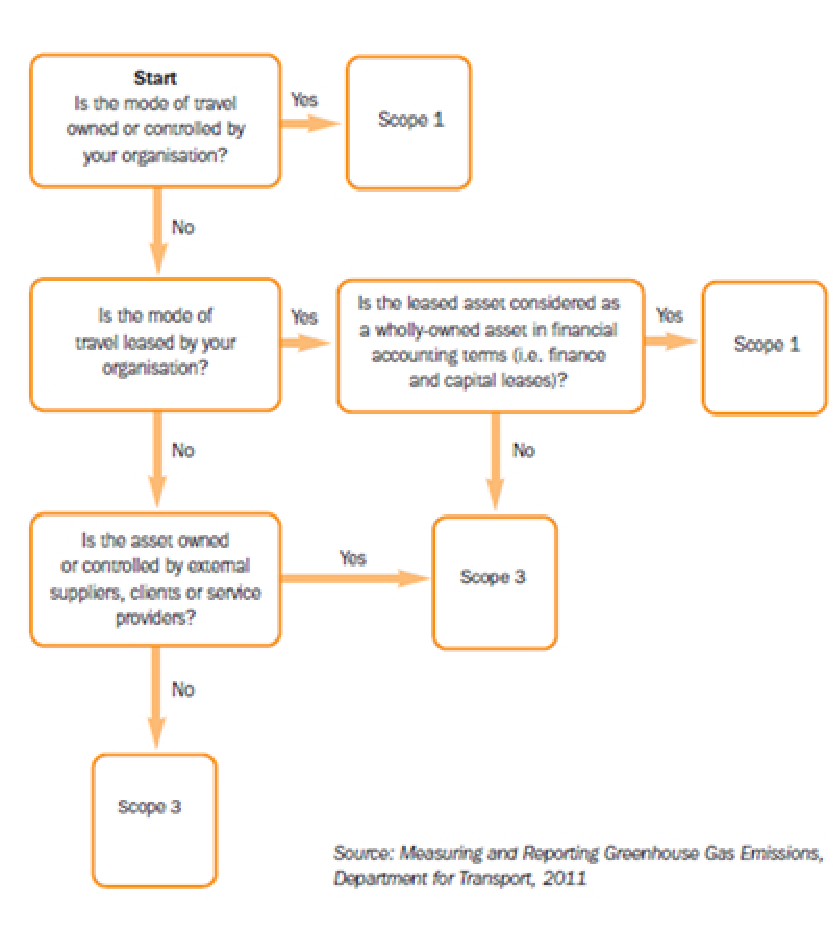
\includegraphics{./Figures/figure17.pdf}
		\rule{35em}{0.5pt}
	\caption[Seperating Scope 1 and Scope 3 Emissions]{How to distinguish scope 1 and scope 3 emissions [24]}
	\label{fig:scope1Scope3}
\end{figure}


\subsubsection{Travel emissions calculation}

The process of calculating emissions caused by travels is the same with what we have presented earlier. As far as travels are concerned, the type of transport mean determines the emission factor that will be used in the calculation formula.


\begin{flushright}
Sunil Patel: \href{http://www.sunilpatel.co.uk}{www.sunilpatel.co.uk}
\end{flushright}
 % Introduction

%% Chapter 2

\chapter{Background} % Write in your own chapter title
\label{Background}
\lhead{Chapter 2. \emph{Background}} % Write in your own chapter title to set the page header

\section{Introduction}

In this chapter we will present the background research pertaining to the theory that underpins the development of our web application. In particular, we describe the core principles of the provenance and carbon footprint theory. The chapter ends with a description of similar application and the tools that were utilized for the implementation of the application.

\section{Provenance of Electronic Data}

A significant factor when buying a piece of artwork is the knowledge of the derivation of that item, as well as, the chronology of the ownership. This has been extensively described with the term provenance and is important for various reasons, chief of which is the fact that it can help us trace the whole history of an object and thus determine the authenticity and establish its historical importance.  Ultimately, one can use this information to determine the value of a work of art.
The same concept has been applied to digital resources or digital information that is generated by computer applications\cite{reference5}. More specifically, in computer science, we refer to provenance of a piece of data, as the process that led to that specific piece of data\cite{reference1}. Moreover, any other data or hardware or user interaction that took part in the computational process, belong to the provenance of that piece of data. In general though, the description of such derivation may be represented in any form based on users' personal interest\cite{reference9}.

Figure \ref{fig:cloudProvTheory} displays the tag cloud for the literature research presented in this section.

\begin{figure}[htbp]
	\centering
		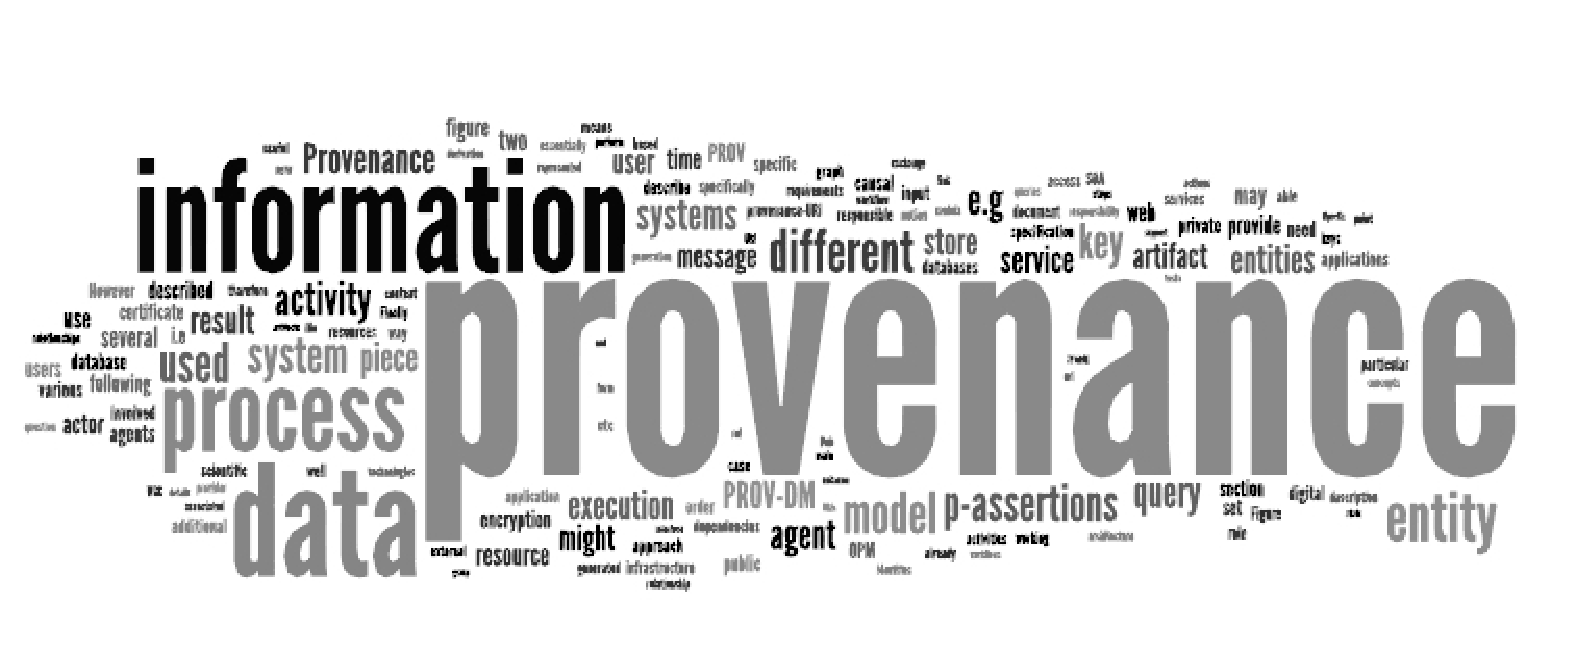
\includegraphics[scale=0.60]{./Figures/chapter2/cloud.pdf}
		\rule{35em}{0.5pt}
	\caption[Provenance Tag Cloud]{Provenance Tag Cloud}
	\label{fig:cloudProvTheory}
\end{figure}


\subsection{Provenance in Scientific Workflows and Curated Databases}

Substantial work on provenance of data has been undertaken by the database, workflow\cite{reference6:5}\cite{reference6:9} and e-science communities.  In particular, the provenance of scientific results can provide proof about the correctness of a result and determine the amount of trust one can place on it\cite{reference5}\cite{reference36}. Representative examples are workflows in the scientific domain. A workflow (e.g. myGrid/Taverna\cite{reference6:18}, Kepler\cite{reference6:6}, visTrail\cite{reference6:13}, chimera\cite{reference6:12} etc), essentially, has been proved to be a successful way to perform complex data processing tasks. Figure \ref{fig:scientificWorkflow}, illustrates an example of a typical workflow. Boxes are used to indicate data processing steps and arrows illustrate the data flow. Each task may take input data from the preceding task, user interactions or external sources (database, external tools).  During a typical workflow run, the means (e.g. input data, user interactions, user parameters etc.) that are involved in the actual derivation of a result, are not recorded whatsoever.  However, the lack of such provenance information makes the outcome of complex analysis difficult to interpret and reproduce. Thus, making these systems provenance-aware will address several issues they suffer from. First of all, scientists will be able to evaluate the correctness of the final workflow output and avoid the duplication of efforts. Furthermore, such provenance information might cater with means for quick troubleshooting or even optimize the whole workflow process\cite{reference1:278}.

\begin{figure}[htbp]
	\centering
		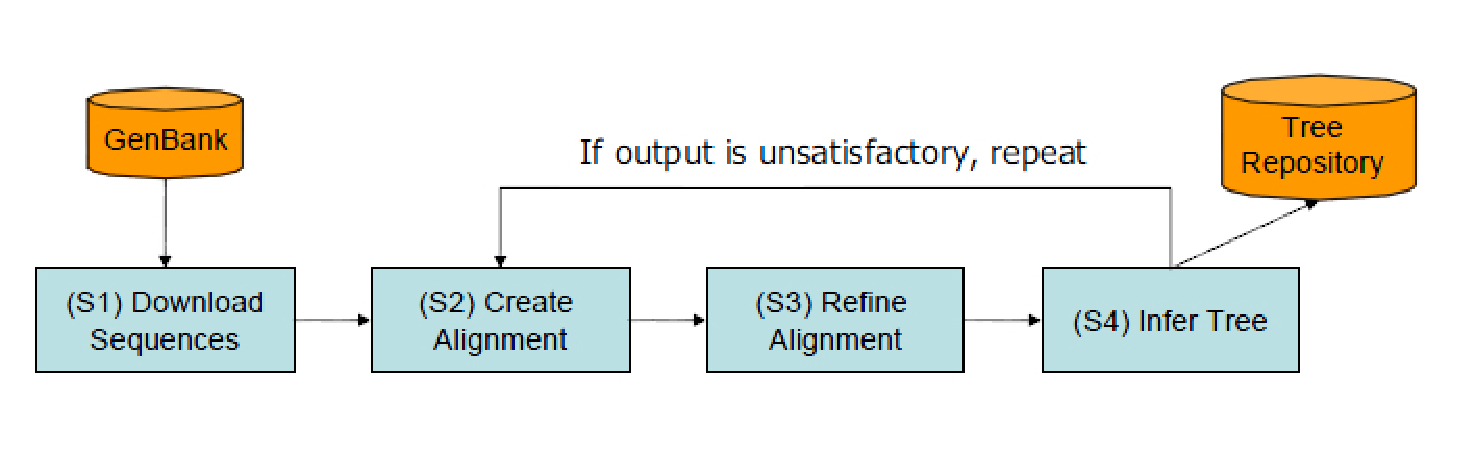
\includegraphics[scale=0.50]{./Figures/chapter2/figure1.pdf}
		\rule{35em}{0.5pt}
	\caption[Scientific Workflow]{Scientific Workflow.\cite{reference6}}
	\label{fig:scientificWorkflow}
\end{figure}


Provenance of data was regarded as an important aspect of the databases storing scientific data. The majority of such databases are usually views of some bigger databases that store raw experimental data. In particular, several scientific stores are populated by the result of queries made to other databases, and are manually updated by several other experts. This sort of databases are commonly known as curated databases\cite{reference1:53}, due to the number of people and/or systems involved in the data insertion and update process. Thus, we can come to recognize that keeping provenance information can help to a great extent to understand the origin of a piece of data, and particularly the process that led to that piece of data. Eventually, we will be able to determine the accuracy, integrity and trustworthiness of data\cite{reference3}.
In the scope of databases, there are two types of provenance that can be observed: "where-provenance", "why-provenance"\cite{reference3:7}. The former identifies the tuples that were involved in the production of a query result; whereas the latter helps identify the original location a piece of information was copied from.

Consider the following example

\begin{figure}[htbp]
	\centering
		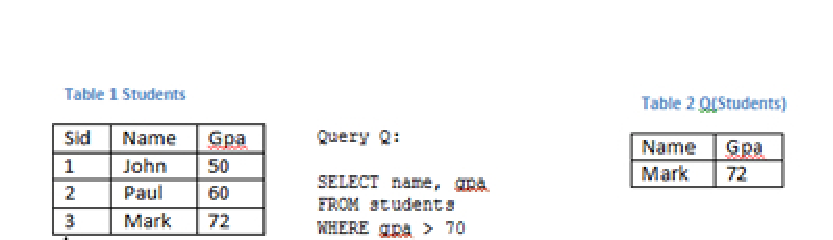
\includegraphics{./Figures/table.pdf}
		\rule{35em}{0.5pt}
	\label{fig:scientificWorkflow}
\end{figure}


Where-provenance can answer to a question such as, where the value gpa ' 72 in the tuple $(mark, 72)$ comes from. The answer would be, that it comes from the field gpa of the tuple with id = 3, in the students table.  Similarly, the why-provenance identifies that the tuple $(3, Mark, 72)$ was the one that contributed to the tuple $(Mark, 72)$ of the query result.
There is a third type of provenance which is called "how-provenance"\cite{reference1:188}. While why provenance identifies the source tuples that justify a query result, how-provenance goes a step further and tries to describe how those tuples were involved in the creation of that result.

\subsection{Provenance Techniques}

In this section we present a classification of different methods that have been used to support data provenance. Figure\ref{fig:provTaxonomy} summarizes the five main aspects according to which we can classify the techniques for data provenance that have been proposed for use in individual domains\cite{reference4}.

\begin{figure}[htbp]
	\centering
		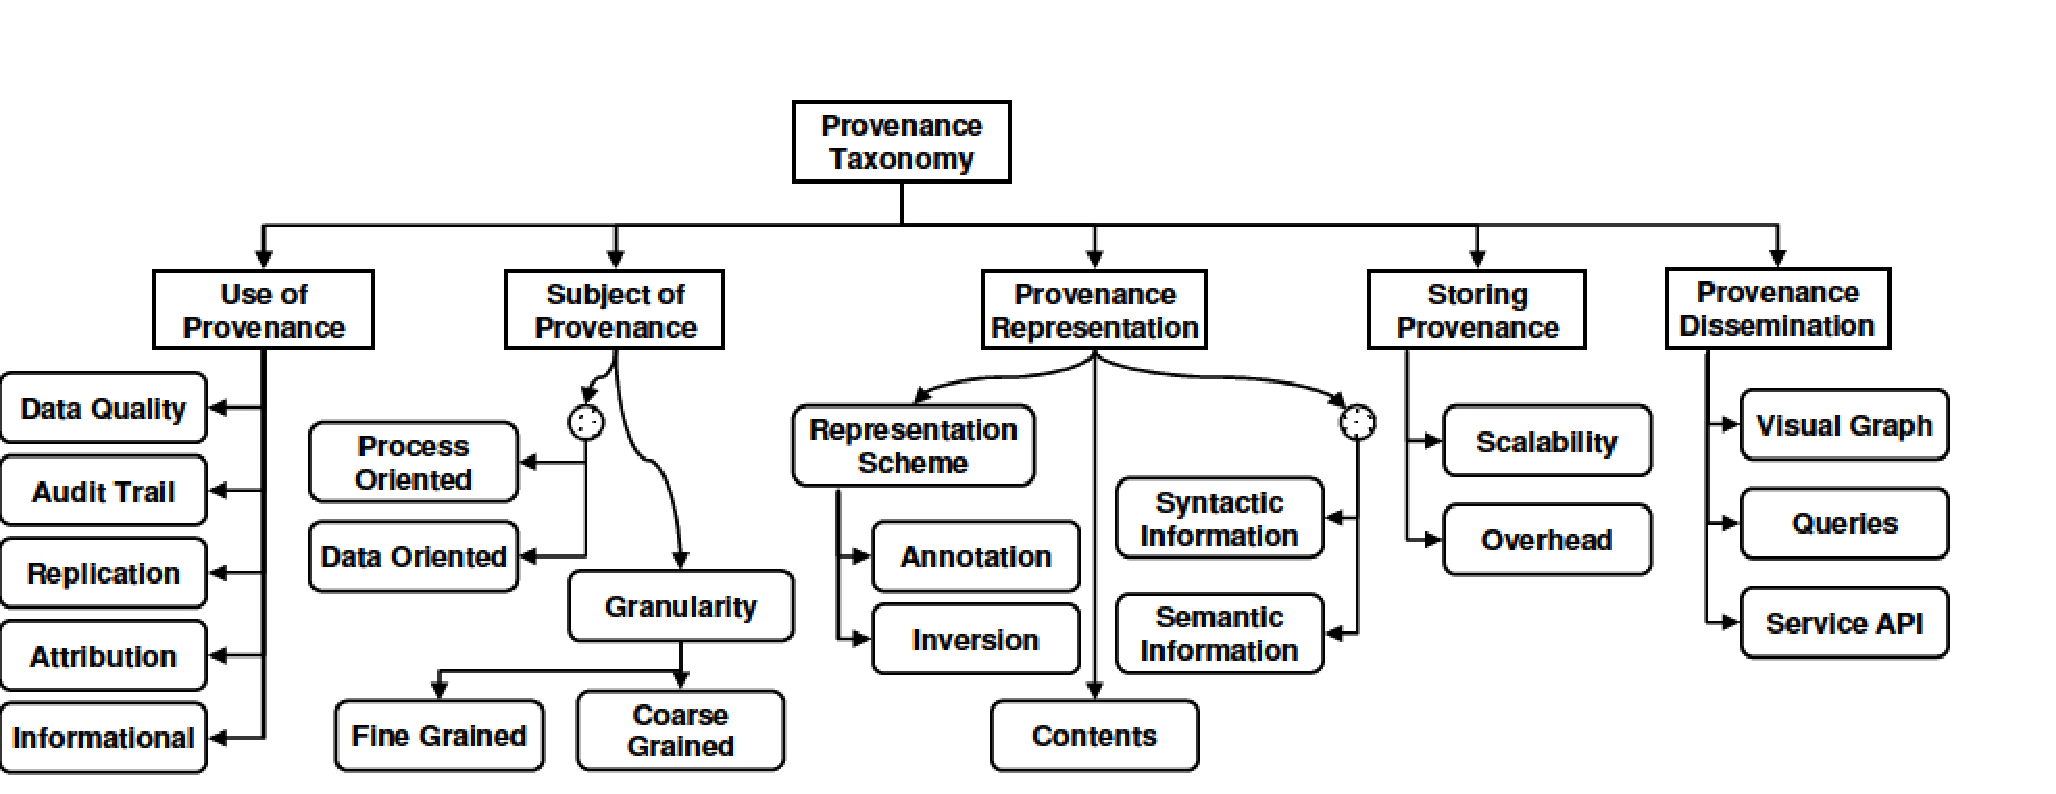
\includegraphics[scale=0.35]{./Figures/chapter2/figure2.pdf}
		\rule{35em}{0.5pt}
	\caption[Taxonomy of Provenance]{Taxonomy of Provenance\cite{reference4}.}
	\label{fig:provTaxonomy}
\end{figure}

\subsection{Subject and Granularity of Provenance Information}

When designing a provenance-aware system, one should specify the subject of provenance - the provenance of what? -  as well as the level of information detail.

Simmhan, et al.\cite{reference4} introduce two models of provenance: in a data-oriented model, the provenance of data is compiled explicitly in the form of metadata. For example, a directed acyclic graph (DAG)can explicitly present the provenance of a piece of data, by simply describing the process that led to its current state.  Contrary to that, the process oriented model suggests that the deriving processes are entities for which provenance is recorded.  Hence the data provenance is implicitly determined by examining the inputs and outputs of those processes.

The granularity refers to the smallest piece of information that provenance is tracked for. For example, in a relational database we can decide to track provenance to the level of rows or cells. Essentially, the system requirements need to determine the level of granularity.


\subsection{Provenance Representation}
There are two major approaches for computing data provenance\cite{reference5}: (i) non-annotation (or inversion method) approach and (ii) annotation approach.

\begin{figure}[htbp]
	\centering
		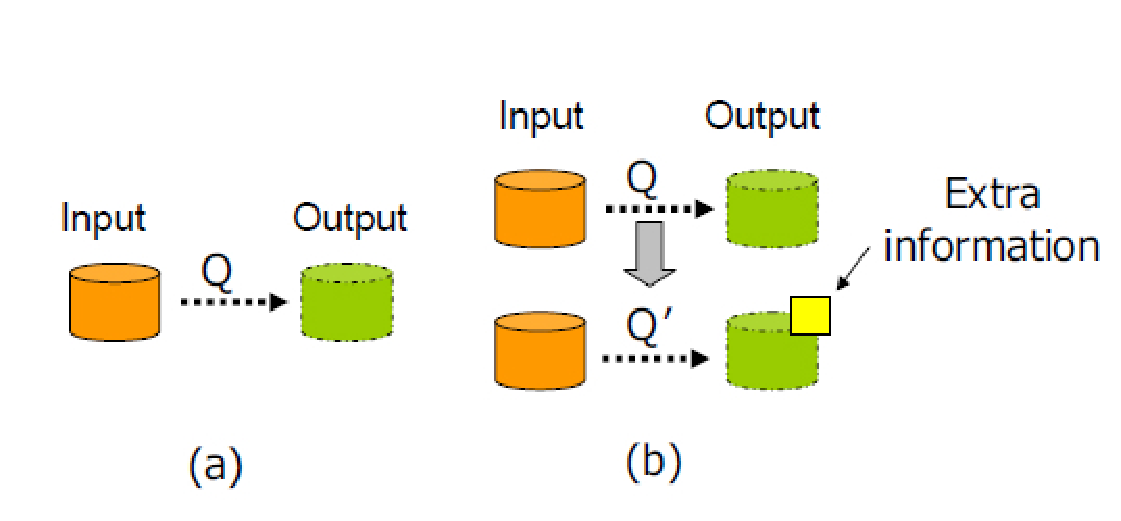
\includegraphics[scale=0.5]{./Figures/chapter2/figure3.pdf}
		\rule{35em}{0.5pt}
	\caption[Provenance Represantation]{(a) Non-Annotation (NA) approach, (b) Annotation (A) approach\cite{reference5}.}
	\label{fig:provRepresentation}
\end{figure}

Consider the example in figure\ref{fig:provRepresentation}.  Q is the transformation function (i.e. query) that acts upon an input database with the aim to generate an output database. This is an example of a non-annotation approach whereby the provenance of the data product (i.e. output database) is computed by analyzing the input and output database, and the definition of Q (e.g. by analyzing the underlying algebraic structure of the query\cite{reference6:18}). On the other hand, the annotation approach is slightly different. Provenance is determined by collating extra information in the form of annotations and descriptions about other resources. In this approach, provenance is serialized in a machine readable format (e.g. xml, rdf/xml).



\subsection{Provenance Dissemination}

Regardless the representation format of provenance, one should be able to view and act upon this captured information. A system needs to provide access and present provenance in both, a user and machine friendly manner. A common way is to visually represent provenance graphs. However, there is a significant caveat. Big provenance graphs are not intuitive and make it difficult for a user to interpret. Hence, this approach is not scalable. A better solution is to support a query engine which can extract smaller parts of a provenance graph.

\subsection{Provenance open data models}

In the previous section we examined how provenance systems have been integrated within scientific workflows and database management systems. Such systems, though, have full control of the information they process and store and thereby they track provenance within their own scope. Architecture like that, promotes tight coupling between various systems components (e.g. provenance system, execution environment etc.)\cite{reference8}

In the era of distributed systems, interoperability is a significant factor that needs to be considered. To that end, systems should adopt mechanisms and techniques that utilize open and technology agnostic models. Several approaches for promoting interoperability rely on an infrastructure that supports several provenance stores\cite{reference8:55}\cite{reference8:56} which offer long-term persistent storage of provenance information. Nevertheless, the representation of the provenance information should be described in a coherent way, regardless of the technologies involved.

The intent of this section is to summarize some early attempts for designing a common provenance model, as well as, the current W3C provenance data model (by the time of this writing, the W3C provenance working group\footnote{\url{http://www.w3.org/2011/prov/wiki/Main_Page}} has published a working draft of the specification)


\subsubsection{Provenance in Service Oriented Architecture (SOA)}

Service oriented architecture (SOA) is an architectural style that has been successfully used in distributed systems. The major advantage of a SOA based system is the loose coupling between various software components, which minimizes the system development time, as well as, the maintenance cost. Applications following the SOA approach are mainly composed dynamically by utilizing services available in a network\cite{soa} . Thus, the need of a shared and technology-agnostic data model is critical for such systems to be able to manage provenance information.

One of the early attempts to integrate provenance systems into SOA applications was the PASOA approach\cite{reference32}. According to the PASOA model, provenance information is described with the notion of provenance assertions (p-assertions)\cite{reference9}. P-assertions are, essentially, assertions made by individual services about their involvement in a process execution. Furthermore, they are the main constituents of a process documentation, which in order, provides with description about what happened at execution time (e.g. which algorithms, data sets or services were involved).

Something that is noteworthy at this point is that the full details of the process that brought a data item to its current state, can considerably be huge (theoretically can trace back to the big bang\cite{reference1}). For example, the full provenance of a result produced by a service that calculates the carbon footprints of individuals might include descriptions of the algorithms that were used, users' input, carbon emission calculation methods, data compiled by external devices (e.g. Gps) and so forth. However, this amount of information might be frustrating for a user who wants to obtain the provenance of a specific piece of data. This fact unveils the need of a query engine where users can make customized queries, so that they can get the information they need and avoid information overload.

During a process execution, there are various tasks carried out. For example, different services might interact with each other by exchanging messages (e.g. SOAP messages) or a single service might apply different transformation functions to input data. As a result, the content of p-assertions can vary. We have three distinct categories of p-assertions based on the content of the provenance information that is being captured.

\begin{description}
  \item[Interaction p-assertions]
         It is an assertion that describes how data flows among the various services in a SOA system. An interaction p-assertion consists of an interaction key that identifies an interaction (i.e. source and destination services), as well as, the content of the message itself (e.g. content of SOAP message)
  \item[ Relationship p-assertions]
      Assertions about how data slows throughout a single service. They can essentially, describe the function or algorithm that was applied to input data, in order to produce the output message.

  \item[Service-state p-assertions]
        During a single execution, a service has a specific internal state. For example, information such as, CPU time used by a service, available space on the disk, user logged in, local time, might be useful to make various interpretations about the computational result.  P-assertions demonstrating all these information are called service-state p-assertions.
\end{description}

The aforementioned p-assertions describe the steps in the history of a process execution and can be visualized as directed acyclic graphs (see figure\ref{fig:provGraph})

\begin{figure}[htbp]
	\centering
		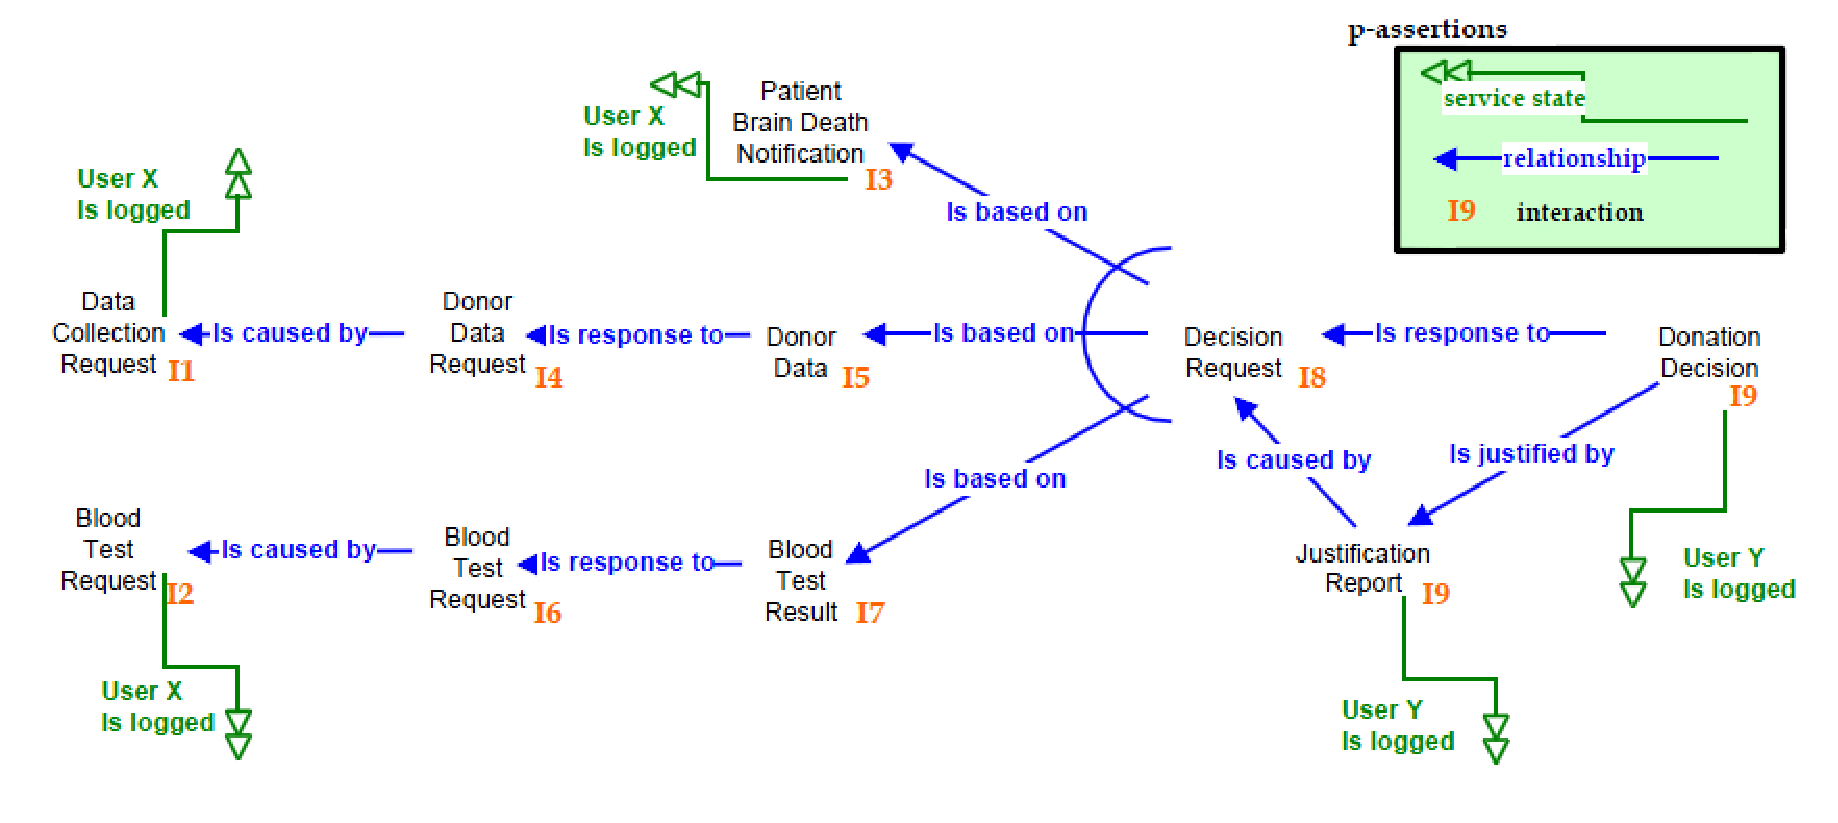
\includegraphics[scale=0.35]{./Figures/chapter2/figure4.pdf}
		\rule{35em}{0.5pt}
	\caption[Provenance Directed Graph]{Provenance Directed Graph\cite{reference9}}
	\label{fig:provGraph}
\end{figure}


\paragraph{Provenance life-cycle}

In this section we briefly describe the different phases that constitute p-assertions life cycle\cite{reference10}. More specifically, p-assertions pass through four distinct phases, which we outline below.
\begin{enumerate}
  \item
        \textbf{Creating p-assertions:} As we have already mentioned, services are responsible for creating p-assertions. While execution precedes each service can only describe its own involvement in the process execution.
  \item
        \textbf{Recording p-assertions:} A provenance store, as described earlier, offers a long-term persistent storage for p-assertions. Hence, after they are created, p-assertions have to be stored in a provenance store, for future use.
  \item
        \textbf{Querying p-assertion:} A provenance store offers a helpful mechanism for obtaining the provenance of a specific piece of data. More specifically, a user can compose queries that will bring the p-assertions according to the users need. In essence, the query will be executed over a process documentation that embraces all the p-assertions.
  \item
        \textbf{Managing p-assertions:} P-assertions may be stored in a provenance store for a long period of time. They therefore may need to be managed over the course of time.
\end{enumerate}

A complete provenance system has to support all those phases of the provenance life-cycle.

\paragraph{A Conceptual Provenance Architecture}

In the previous section we outlined the four main phases of the provenance (or p-assertion) life cycle. For a system to be able to support those phases, a logical architecture that will consist of appropriate system components, has to be designed. Groth et al.\cite{reference10} suggest generic provenance system architecture (see figure\ref{fig:provArch}).

\begin{figure}[htbp]
	\centering
		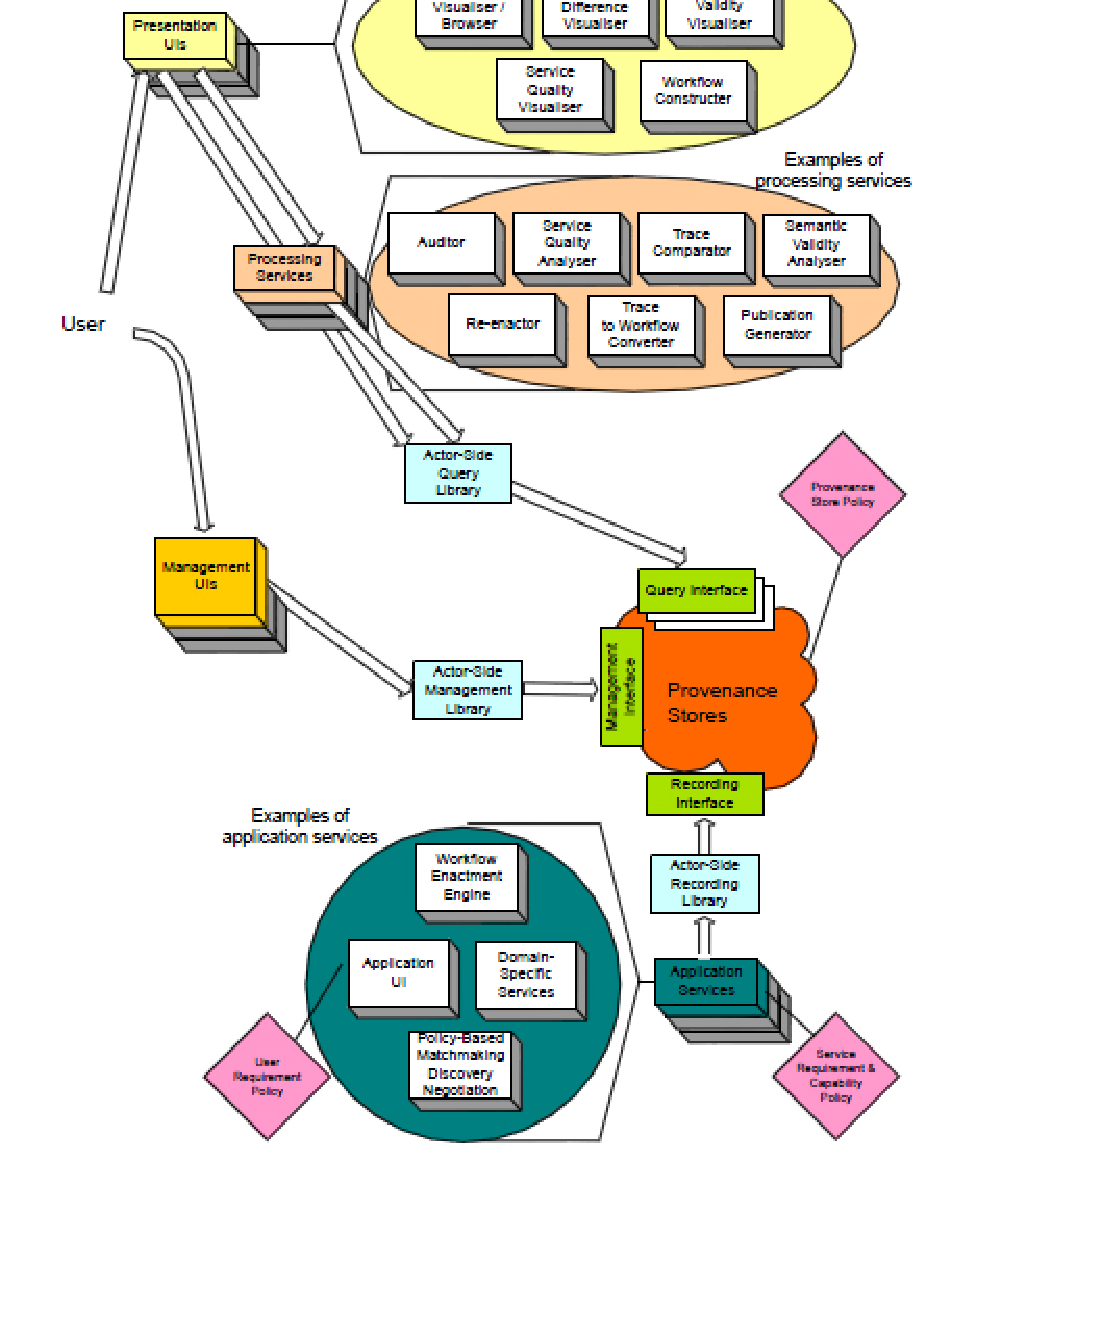
\includegraphics[scale=0.80]{./Figures/chapter2/figure5.pdf}
		\rule{35em}{0.5pt}
	\caption[Architecture of Provenance-Aware Application]{Architecture of Provenance-Aware Application.\cite{reference10}}
	\label{fig:provArch}
\end{figure}

In this architecture, we can observe four different actors that are involved in the provenance life-cycle

\begin{description}
  \item[Application actor]
        It is the system component that processes the business logic of the application.
  \item[Provenance store]
        This is the central point in the architecture. As we have already described, it is the responsibility of the provenance store to persist and provide access to the recorded provenance information.
  \item[Querying actor]
        This is the part of the system that communicates with the provenance store by issuing provenance queries.
  \item[Recording actor]
        While the querying actor sends queries to the provenance store, the recording actor populates it by submitting p-assertions.
  \item[Asserting actor]
        This is the actor that creates appropriate p-assertions while the execution proceeds.
  \item[Managing actor]
        An actor that performs managing tasks in the provenance store.
\end{description}

It is obvious that the provenance store is the key actor in the provenance lifecycle. It interacts with several other system components and therefore should provide appropriate interfaces to facilitate those interactions.

\begin{itemize}
  \item
        A \emph{recording interface} which gives access to recording actors so that they can submit p-assertions.
  \item
        A \emph{query interface} which is the entry point for query actors so that they can issue provenance queries and get back query results.
  \item
        A \emph{management interface} which allows managing actors to perform managing tasks in the store.
\end{itemize}


\subsubsection{Open Provenance Model}
The provenance data model we presented earlier, describes a shared model for capturing, recording, exchanging and managing provenance information. However, it is primarily bound to SOA applications, that is, to message exchanging systems. The models that we discuss in this section is the first purely technology agnostic provenance data model.

The Open Provenance Model (OPM)\cite{reference13}\cite{reference34} addresses different provenance interoperability issues by introducing the notion of the provenance interoperability layer\cite{reference1}.

Figure\ref{fig:provAccrossSystems} illustrates a big system which consists of several individual applications. Each of these applications is designed to be provenance aware and makes use of its own provenance store. In a system like that, where information flows across different applications, the history of the derivation of a piece of data (i.e. provenance) might reside across several provenance stores. As a result, one would need to query several provenance stores, to form the whole process execution chain. It is the job of the inter-operability layer to conceal the technology diversity of individual applications and expose provenance data in a uniform manner.

\begin{figure}[htbp]
	\centering
		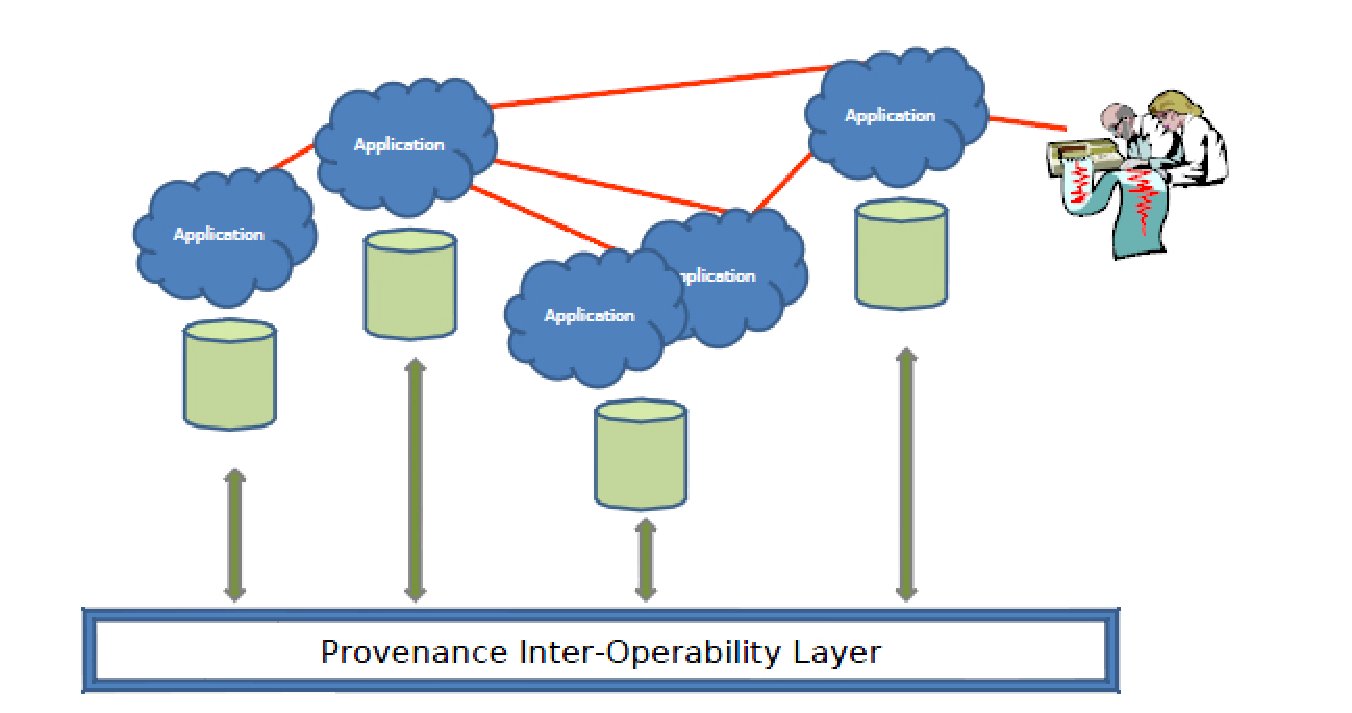
\includegraphics[scale=0.60]{./Figures/chapter2/figure6.pdf}
		\rule{35em}{0.5pt}
	\caption[Cross-System Provenance]{Cross-System Provenance.\cite{reference1}}
	\label{fig:provAccrossSystems}
\end{figure}

The open provenance model utilizes a graph structure to represent a set of causal dependencies\cite{reference13} among its nodes. A set of such dependencies can explain how a digital piece of data, physical resource (e.g. bicycle) or a conceptual entity (e.g. immaterial entity, idea etc.) came to be in a particular state at a specified time.

OPM suggests three types of nodes, which we now present:

\begin{description}
  \item[Artifact]
         A digital, physical or conceptual entity can have different sets of characteristics, at different moments. We call this specific state of an entity, an artifact. An artifact can be viewed as a snapshot of an entity at a given moment; for example, a pdf file at a specific time. States are immutable in that they cannot be modified. Alterations to any characteristic of an entity at a given time result in the generation of a new artifact.
  \item[Process]
        A process refers to an action or a sequence of actions that result in the generation of new artifacts; for example the process of embedding images into a pdf file produces a new pdf file, enriched with multimedia characteristics (i.e. images).
  \item[Agent]
        Agent is an entity which triggers a process. In other words, it is the responsibility of an agent to initiate or terminate a process. Following the example with the pdf file, an agent might be a software component that initiated the process of adding images into the new file.
\end{description}

Nodes in an OPM graphs are connected with each other via causal dependencies. Such dependencies are illustrated with directed edges from the source bode (or effect) to the destination node (or cause).

The OPM model introduces an initial set of causal dependencies which are illustrated in figure\ref{fig:provCausalDependencies}. This is a graphical representation of the causal relationships between artifacts, processes and agents. Artifacts are represented by ellipses; processes are represented by rectangles; and agents by octagons.

\begin{figure}[htbp]
	\centering
		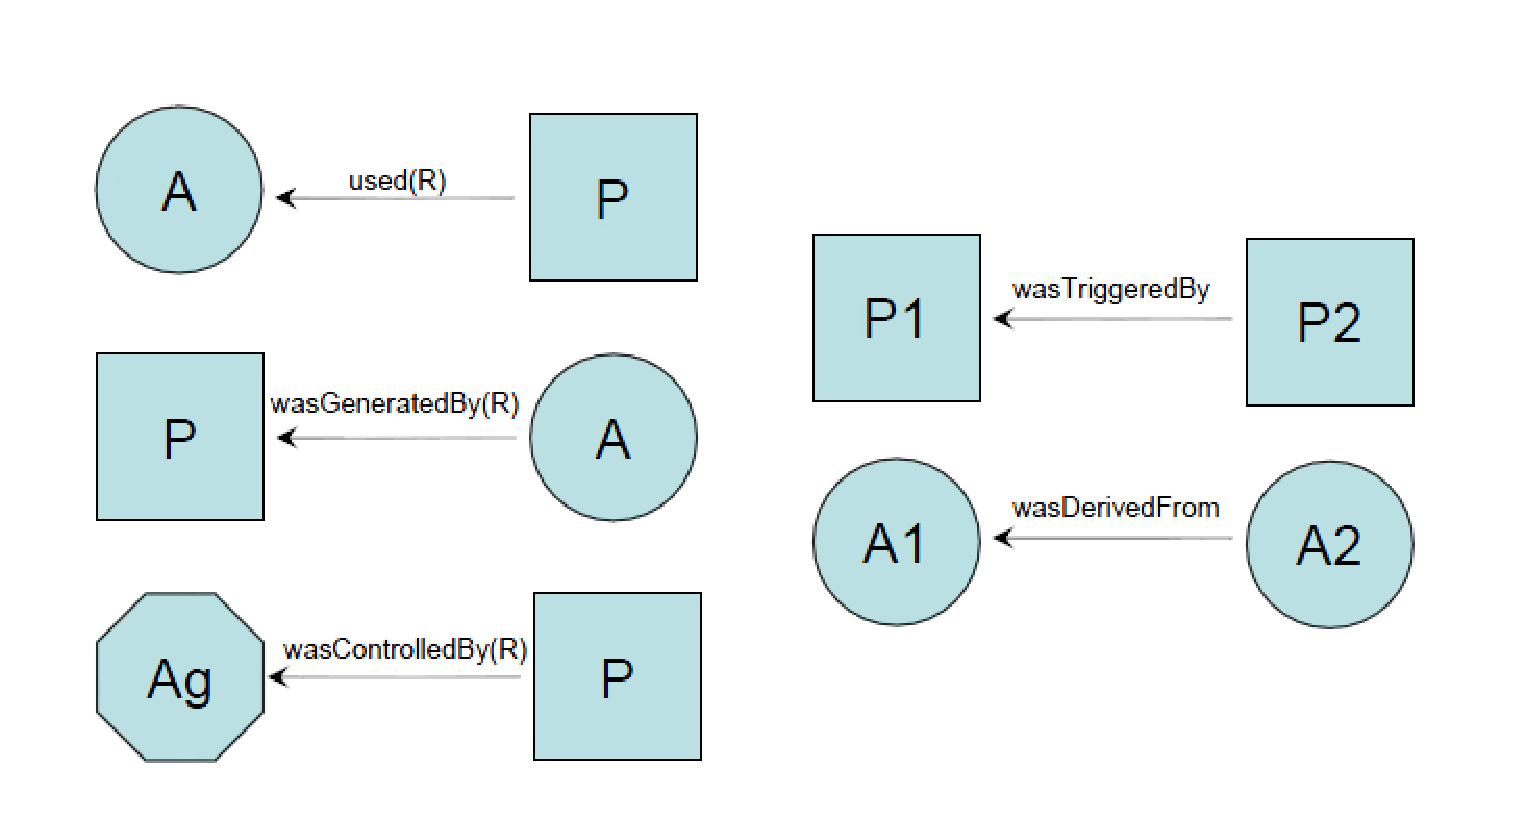
\includegraphics[scale=0.60]{./Figures/chapter2/figure7.pdf}
		\rule{35em}{0.5pt}
	\caption[Provenance Causal Dependencies]{Provenance Causal Dependencies\cite{reference13}. Note that past tense aligns with the notion of process history documentation.}
	\label{fig:provCausalDependencies}
\end{figure}

We observe a set of five types of causal dependencies based on participants.

\begin{description}
  \item[Used]
        A relationship between a process and an artifact denoting that the process used the artifact to produce a result (e.g. a new artifact). The formal definition suggests that the availability of the artifact is critical for the process to complete the execution.
  \item[wasGenerateBy]
        It is a relationship between an artifact and a process, indicating that the artifact was generated by the process. In other words, the existence if the artifact is due to the execution of that process.
  \item[wasTriggeredBy]
        Figure\ref{fig:provCausalDependencies} shows an edge wasTriggeredBy from a process p2 to a process p1. The semantics of this relationship defines that there was some unknown artifact that was generated by some process p1 and was used by a process p2.
  \item[wasDerivedFrom]
        An edge wasDerivedFrom from an artifact node A2 to another artifact node A1 denoted that there was a process that used an artifact A1 to generate an artifact A2. It is a useful relationship, when the actual process of a transformation is unknown.
  \item[wasControlledBy]
        It is a causal dependency between a process and an agent. It simply indicates that the execution (i.e. the start and end) of a process is carried out under the control of an agent.
\end{description}

Note the letter R in the "used", was controlled by" and "was generated by" edges. This is a bit of extra information that is used in the aforementioned relationships to characterize the role of each entity (i.e. artifacts, agents) that is connected to the same process. More specifically, in a "used" relationship, the same process may use several artifacts. However, the nature of each usage might be different; for instance, an online process for searching for news based on a keyword and a specified source uses the keyword with the role "keyword to search" and the source web site with the role "web site to search". Similarly, a process can generate several artifacts with different role each. Following the previous example, the process can produce a news article and a set of additional sources. The former will have the role "article associated with the keyword" whereas the latter will have the role "additional sources to look at". Finally, a process can be controlled by multiple agents, each with a distinct role. In the example of the online news fetcher, the process for searching news can be initiated either by a user via a user interface, or by an external application via an application programming interface (API). The Roles in this case might be "internal actor" and "external actor" respectively.

One of the concepts associated with provenance that we have been constantly highlighting, is the ability to specify the scope of the provenance that is being captured.  A provenance of a piece of data can be expressed in various levels of detail. Furthermore, it can be viewed from different angles and standpoints. To that end, OPM introduces the notion of accounts. An \textbf{account} is regarded as a graph coloring, indicating different provenance sub-graphs which provide details at different level of abstraction.


The concept of accounts is fairly useful and caters users with multiple descriptions of the provenance of the same piece of data.
A final note about OPM concerns the extensibility capabilities of the model. Stronger interpretations of the causal dependencies we described in this section can be used to serve application-specific requirements. A common way to achieve that would be to design an ontology with subclasses of those causal dependencies.


\subsubsection{The W3C Provenance Working Group}
The open provenance model was a good initiative to tackle with inter-operability issues pertaining to the provenance dissemination across multiple platforms. However, as is the case of many widely used technologies, there should be a consensus among different bodies (e.g. industry, academia etc.) about the final specification. For this reason, the provenance working group was formed in the World Wide Consortium (W3C). The group followed the work that was started by the Provenance Incubator Group\footnote{\url{http://www.w3.org/2005/Incubator/prov/wiki/W3C_Provenance_Incubator_Group_Wiki}}. The ultimate goal of the group is to reach an agreement upon the specification of provenance on the World Wide Web.

At the time of this writing, the provenance working group has published a set of specifications which are still on the "working draft" step of the W3C specification approval process. In particular, the specifications that have already been released are:

\begin{description}
  \item[PROV Data Model]
        A data model for describing all the parties that are involved in the generation of a data item\cite{reference15}.
  \item[PROV Ontology]
        A OWL 2 web ontology for expressing the PROV data model. In essence, it is the "vocabulary" that is used by the PROV data model to represent provenance information\cite{prov-ontology}.
  \item[PROV Notation]
        Specification which aims to design the means for a human friendly representation of the information expressed by the Prov data model\cite{prov-notation}.
  \item[PROV Constraints]
         A document that defines a set of constraints that assures the validity of PROV instances (statements). Further, it specifies inference rules for reasoning over PROV instances. This can result in the creation of additional statements implied from the explicitly stated provenance information\cite{prov-constraints}.
  \item[PROV Access and Query]
        A document that describes the means to leverage the existing web infrastructure, in order to query and obtain provenance information\cite{prov-AQ}.
\end{description}

In this section, we will present the PROV data model (PROV-DM). For additional information about the rest specifications, we refer the reader to the official web site  of the W3C provenance working group\footnote{\url{http://www.w3.org/2011/prov/wiki/Main_Page}}


\paragraph{PROV Data Model}
Provenance can be viewed from different standpoints, and therefore various kinds of information can be stored in provenance records\cite{reference14}.

The provenance data model identifies three distinct perspectives of provenance:

\begin{itemize}
  \item
        \textbf{Agent-centered provenance:} emphasis is given on the entities that took part in the generation or manipulation of the data item in question; for example, considering the provenance of a video file in a blog post, we might want to know the person who recorded that video, the person who edited it, and the user who posted it on the blog.
  \item
        \textbf{Object-oriented provenance:} a different perspective suggests that we might want to identify the origin of different parts of a document; for example, in the same blog post, we may want to know that the video was taken from YouTube and the images from Flickr.
  \item \textbf{Process-oriented provenance:} finally, we may want to highlight the actions that were carried out to generate a data item; for example, a visual graph illustrating the connections I have in a social network site may have been generated by invoking a service to pull data from the social network, which then are processed by a JavaScript library for visualization.
\end{itemize}

Regardless the various viewpoints that provenance can be examined, a good data model should provide all the means needed to capture adequate information. To that end, the PROV-DM introduces some key concepts, which we outline in the following lines.

\begin{figure}[htbp]
	\centering
		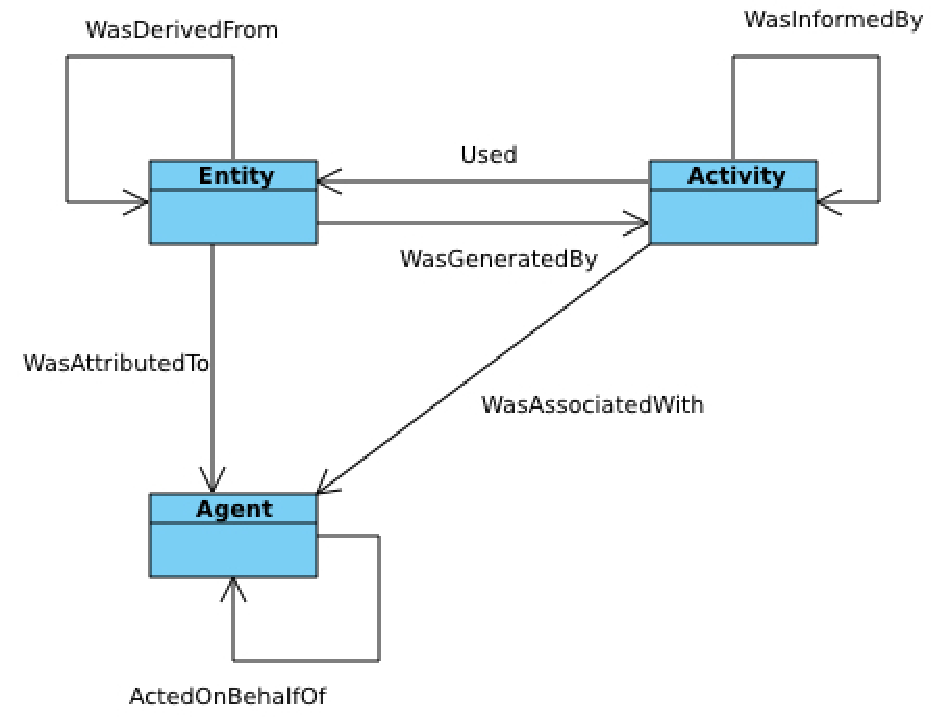
\includegraphics[scale=0.90]{./Figures/chapter2/figure8.pdf}
		\rule{35em}{0.5pt}
	\caption[PROV-DM]{PROV-DM\cite{reference14}. Note that past tense aligns with the notion of process history documentation.}
	\label{fig:provDM}
\end{figure}

An entity is the equivalent to an artifact in the open provenance model. It may refer to a physical, digital or immaterial thing, such as a blog post, a car or a decision. The second, constituent is the activity. This is equivalent to a process in OPM model and represents the derivation of an entity. In particular, it refers to the process of generating a new entity or the transformation of one entity to another; for example, the process of calculating the carbon emissions of an individual based on some input data is regarded an activity. Finally, an agent in PROV-DM is assigned a degree of responsibility for an activity that is being carried out. The concept of an agent is similar to that of an actor in the OPM model, in that it represents a "thing" that is responsible for controlling the execution of an activity. An agent can be a human being, an organization, software or any other entity that may initiate an activity; for example, a JavaScript visualization library can be an agent that is responsible for imitating a graph visualization activity.

At this point we have to note that provenance can be expressed only for entities. However, we can make provenance assertions about an agent, should the agent be declared both as an agent and an entity.
These are the main concepts of the PROV-DM data model. In addition to that, the data model encompasses several other relationships (for additional information, refer to the official document\cite{reference15}).


\paragraph{Entity Generation and Usage}

An activity in PROV-DM can be related to an entity in two different ways.  First of all, the effect of the actions that comprise an activity is usually the generation of new entities. Hence, entities exist due to activities existence; for example, assembling car parts brings a car into existence. Additionally, activities can use entities, often during the process of generating other entities; for example, a visualization activity can use some datasets stored in a database, in order to create a chart. These two relationships are represented in the PROV-DM with the terms \emph{wasGeneratedBy} and \emph{used} respectively

\paragraph{Agents' Responsibility}

Agents can be associated with entities, activities or other agents. Relationships between entities and activities come in the form of responsibility that an agent has over them. We have already highlighted that agents are responsible for the execution of an activity. A responsibility might refer to an agent initiating or terminating an activity. For example, in PROV-DM we say that an activity was associated with an agent. Similarly, an activity can be responsible for an entity. This form of responsibility can be interpreted as the attribution of an entity to an agent. In other words, the was AttributedTo relation, from an entity to an agent, denotes that an agent was responsible for an activity that was the cause for this entity to be created. This is useful relation when the activity is unknown or of a little significance. Finally, PROV-DM provides mechanisms to express relations between two agents. In particular we say that an agent can act on other agent's behalf; for example, an employee can be designated by the company to perform some actions on their behalf.

\paragraph{Entity Derivation}

The last core relationship defined by the PROV-DM is a relation between two entities. The existence of an entity might often be due to some other entity that was used by the activity that generated it. In that case, it is said that one entity was derived from another entity. A special kind of such relation is the "was revision of"; for example, the PROV-DM specification may go through multiple revisions over the course of time. Such relation can be useful to examine the changes that had been brought across the different revisions of a document.

\paragraph{Roles}

Recall the notion of roles in the OPM model. The PROV-DM has adopted the same notion to characterize relationships between entities and activities. In particular, a role specifies how an entity was used or generated by an activity. Similarly, roles can specify the nature of agents' involvement in an activity. It is obvious that roles are application specific, and therefore are not specified by PROV-DM.

\paragraph{Plans and Accounts}

Activities may consist of numerous steps and procedures. For instance, an online tutorial for publishing links data on the web illustrates several steps that should be taken. In PROV-DM there is a specific term to represent this set of actions. In PROV-DM language, this term is called \textbf{plan}. Plans are entities, therefore we can describe provenance for them.
Finally, one would wonder how we can trust the provenance information about a resource. In fact, this is a plausible question, since anyone can make provenance assertions about any entity. The PROV-DM supports a means to address this issue, namely it includes the notion of accounts. In essence, an \textbf{account} is an entity that contains some provenance information, and because it is an entity, we can express a provenance for it. That is to say, provenance of provenance can be expressed.

\begin{verbatim}
Entity(ex:w3c-publication.pn, [prov:type="prov:Account" % % xsd:QName])
wasAttributedTo(ex:w3c-publication.pn, w3:consortium.)
\end{verbatim}

In the above example, which is written in PROV-Notation, we have explicitly declared the "ex:w3c:publication.pn" provenance description. We then state that "w3:consortium" agent was responsible for its generation.

In this section we presented only the core principle of the PROV-DM specification. However, the whole specification is very rich and consists of many more concepts and definitions. For this reason, we would recommend the reader to visit the provenance working group web site and read the whole set of PROV specifications.

\subsection{Security}

A provenance-aware system is, essentially, capable of recording and storing provenance information about different assets that reside in the system. As we have already discussed, this sort of functionality is accomplished with the aid of a data model, which defines the way that provenance information is represented internally. Further, the presence of a provenance store guarantees the long-term storage of provenance information, as well as, provides a means for querying the store\cite{reference19:5}. The result of a provenance query is a causal graph or provenance graph, which illustrates the provenance information in a way that can be viewed an analyzed.

Throughout the process described above, there is nothing that guarantees the quality and integrity of provenance information. To address this problem a framework that will consider all the security-related aspects of the provenance information, have to be devised. Such framework can leverage existing technologies (e.g. cryptography), that have been successfully applied on the web.
We will start our discussion by introducing some fundamental concepts and technologies pertaining to the security in computer systems.

\subsubsection{Fundamental concepts}

A discussion about security issues concerning the communication between different entities, which exchange some sort of information, should start by defining some initial security requirements. More specifically, there are five requirements that a secure system must provide.

\begin{description}
  \item[Confidentiality]
        A system has to guarantee that all the information that is being exchanged between different entities is protected against eavesdroppers; for example, the information that we exchange when purchasing a product on eBay, should not be wire tapped by anyone.
  \item[Integrity]
        A message sent from one entity to other should not be altered, whatsoever; for instance an order sent to eBay has to remain intact while traveling through the wire.
  \item[Authentication]
        A mechanism that blocks unauthorized users from accessing the systems data and functionality. Access should be granted only to those users who can provide adequate information, in order to prove their identity; for instance In order to be able to perform a purchase action on eBay, one should provide his credentials.
  \item[Non-repudiation]
        An important requirement in the communication between two entities is to be able to prove that a message was indeed sent by its sender; for example, once a user submits a purchase order, she cannot claim that has not done so.
  \item[Authorization]
        This requirement is also known as \emph{access control}. It is, essentially, a mechanism that determines the sort of access that a user can have on systems resources; for example, as an ordinary user, I cannot modify the systems database by deleting items that I am not authorized to delete.
\end{description}

\subsubsection{Cryptography}

Authorization and authentication are two requirements that can be achieved fairly easier that the rest. To support authorization, a system can simply apply one of the proposed models for access control (e.g. MAC\cite{mac}, DAG\cite{dag}, RBAC\cite{rbac}, ABAC\cite{abac} etc.). Similarly, authentication can be achieved by leveraging the current web infrastructure and the HTTP protocol capabilities (e.g. content negotiation). To meet the rest requirements, a system can use cryptography technics. More specifically, confidentiality can be ensured with encryption\cite{cryptography} whereas non-repudiation with digital signatures\cite{digitalSignatures}. Finally, integrity can be guaranteed with either of those two technics. We review those technologies in the following sub-sections.

\paragraph{Symmetric Encryption}

This type of encryption requires that the entities that participate in a message exchange communication use the same key for the encryption and decryption phase. For example, figure\ref{fig:symmetricEncryption} illustrates a message exchange scenario.

\begin{figure}[htbp]
	\centering
		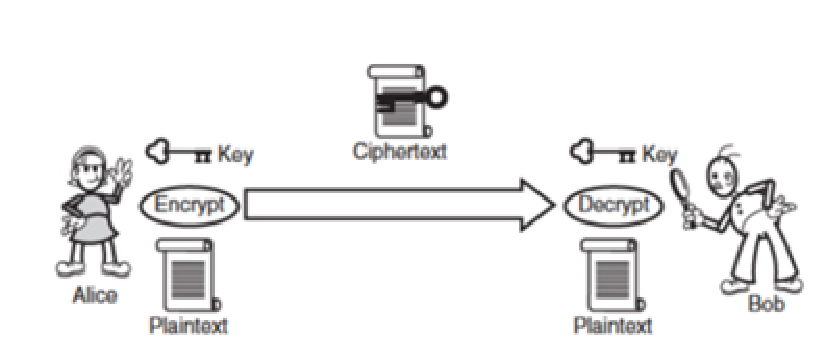
\includegraphics{./Figures/figure12.pdf}
		\rule{35em}{0.5pt}
	\caption[Symmetric Encryption]{Symmetric encryption\cite{Graham:2001:BWS:559927}.}
	\label{fig:symmetricEncryption}
\end{figure}

In this scenario Alice wants to send a message to Bob. As shown in the figure, she encrypts the original data (plaintext) with a private key, and sends it to Bob who decrypts the encrypted message (cipher text) using the same private key. Some of the algorithms that can used to encrypt data are: 3DES, DES, AES, RC4

\paragraph{Asymmetric Encryption}

Asymmetric encryption is more flexible, in that two different keys are used: a private and a public key; for example, figure\ref{fig:asymmetricEncryption} demonstrates the same scenario but now an asymmetric encryption is used. Alice uses Bob's public key to encrypt the plaintext and sends it to Bob, who decrypts the cipher text using his private key.

\begin{figure}[htbp]
	\centering
		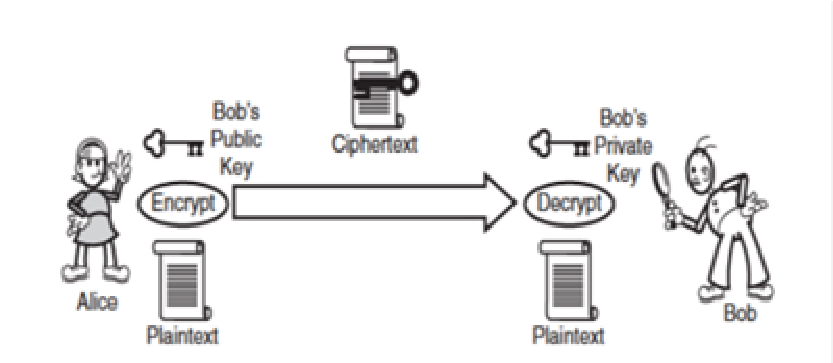
\includegraphics{./Figures/figure13.pdf}
		\rule{35em}{0.5pt}
	\caption[Asymmetric Encryption]{Asymmetric encryption\cite{Graham:2001:BWS:559927}.}
	\label{fig:asymmetricEncryption}
\end{figure}

\paragraph{Digital Signature}

Integrity and non-repudiation can be guaranteed with the use of digital signatures. To better describe this technology look at figure\ref{fig:digitalSignature}. Alice has a pair of private and public keys.

\begin{figure}[htbp]
	\centering
		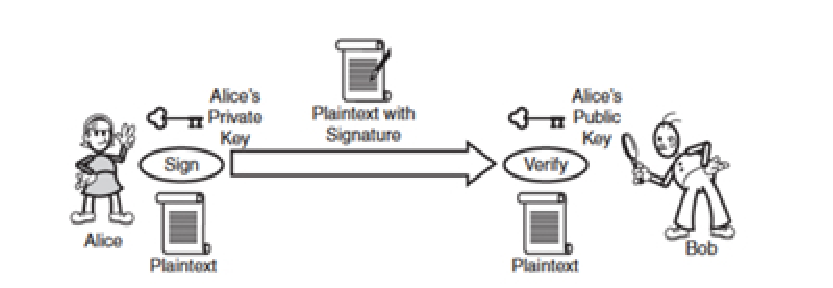
\includegraphics{./Figures/figure14.pdf}
		\rule{35em}{0.5pt}
	\caption[Digital Signature]{Digital Signature\cite{Graham:2001:BWS:559927}.}
	\label{fig:digitalSignature}
\end{figure}

She creates a signature value with her private key and sends it to Bob along with the original plaintext. On the other side, Bob uses Alice's public key to generate a signature value based on the content of the message he received. He then can compare the two signatures to verify the integrity if the incoming message.

\paragraph{Asymmetric versus Symmetric Encryption}

A noticeable caveat of the symmetric encryption is the key distribution problem. Both participants need the same key to encrypt and decrypt a message; therefore they need to somehow exchange it. This has to be done carefully to avoid malicious attackers from stealing the transmitted keys. On the other hand, the most evident downside of the asymmetric encryption is that it exhibits very poor performance. Asymmetric encryption is much slower that symmetric.

\subsubsection{Security protocols}

SSL is probably the most prevalent security protocol for distributing keys in a safe mode. It, essentially, defines the requirements for a secure exchange of keys between two parties. The main steps described by the protocol are the followings:

\begin{enumerate}
  \item
        The client communicates with a server
  \item
        The server responds back by returning its certificate
  \item
        The client computes a random number which represents a seed for generating private keys. He then encrypts this number using the public key included in the server's certificate and sends it to the server.
  \item
        The server obtains the random number by decrypting the received message
  \item
        Ultimately, both parties have the same seed; they therefore can create the same private key.
\end{enumerate}

\subsubsection{Public key infrastructure}

As described earlier, in the asymmetric encryption we do not need to bother about how to distribute private keys, since we can share a public key. However, it is critical that we associate the public key with a particular party. In other words, the owner of the public key has to be identified. To that end, the \textbf{Public Key Infrastructure} (PKI)\cite{pki} has been designed. The main constituent of PKI is a certificate, which is a digital resource that associates a participant to a public key. This certificate is digitally signed and issued by a trustworthy third-party authority, which is called \textbf{Certificate Authority (CA)}. There is a relatively small number of CAs in PKI and they can issue certificates to other certificate authorities.

To better describe this infrastructure, consider the following example. Figure\ref{fig:pki} illustrates a typical PKI scenario.

\begin{figure}[htbp]
	\centering
		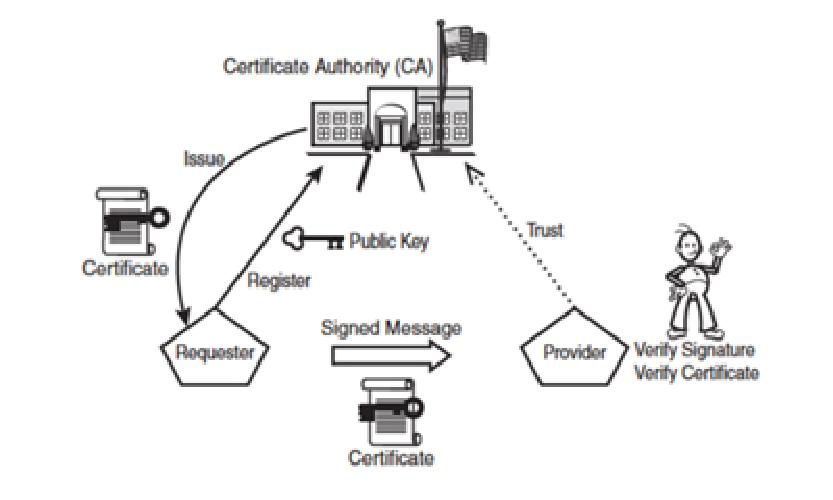
\includegraphics{./Figures/figure15.pdf}
		\rule{35em}{0.5pt}
	\caption[Public Key Infrastructure]{Using certificate for a digital signature\cite{Graham:2001:BWS:559927}.}
	\label{fig:pki}
\end{figure}

Alice signs a message with a private key and sends it to Bob along with a certificate.  Bob creates a signature value using the public key contained in the certificate. But before that, he has to verify that the certificate is signed by a trustworthy certificate authority.

\subsection{Publishing and querying provenance information}

An important task for a provenance-aware system is to capture and store provenance information. An equally crucial feature is for someone to be able  to locate that information and ultimately query and retrieve it some format\cite{reference35}.  For that reason, an infrastructure should be supported so that external applications, users or the application itself could reuse the captured provenance information. Such infrastructure should resolve the problem of locating, retrieving and querying that information. The most appropriate solution is to leverage the current web infrastructure, as well as, some semantic web technologies. In more detail, \emph{uniform resource identifiers} (URIs)\footnote{\url{http://www.w3.org/TR/uri-clarification/}} can be assigned to provenance information (provenance-URIs), as well, as, its constituents (i.e. entities, activities and agents). Any application can then perform HTTP GET\footnote{\url{http://www.w3.org/Protocols/rfc2616/rfc2616.html}} requests to access the information that is associated with the Uri in question\cite{prov-AQ}. This is similar to the way URIs are dereferenced when accessing web resources. Nevertheless, it not a strict requirement to assign unique URIs, due to the difficulties that such process has. Thus, alternative methods can be provided to facilitate the same functionality (we discuss them further in this section).

Locating provenance information is crucial and indispensable in scenarios where a provenance-URI is unknown. In such occasions, an application or a user has to provide some additional information to a provenance provider, which can be a third-party application. According to the submitted information, a provider can locate the provenance-URI and/or the provenance information itself.

Provenance information, as already mentioned, consists of causal relationships between entities, activities, and agents. As such, it is a requirement that one can retrieve descriptions about those resources. The concept is similar, URIs (entity-URIs) can be assigned to those resources and one of the following mechanisms can be provided:

\begin{itemize}
  \item
        In the case where the requester knows the entity-URI, a simple HTTP mechanism can be used to access the dereferenced content. More specifically, if a resource is accessible via an HTTP GET request, an additional link header denoting the URI where provenance for that resource is located can be injected into the header of the response.

\begin{verbatim}
Link: provenance-URI; rel="provenance"; anchor="entity-uri"
\end{verbatim}

        The \emph{entity-URI} indicates the location where additional description for that resource can be obtained, whereas the provenance-URI identifies the location of the provenance information which the entity is part of. If the provider though, does not know anything about provenance locations, it can point to a third-party provider or a provenance service. In that case, the link header is slightly different.

\begin{verbatim}
Link: provenance-service-URI; rel="provenance-service";
anchor="entity-uri"
\end{verbatim}

        The \emph{provenance-service-URI} will, essentially, return a service description that will aid a client to locate a provenance-URI or fetch provenance information for the entity in question.

  \item
        For resources that are presented in HTML, provenance-URI can be included within the document. The simplest way to do that would be to use the \textless Link\textgreater html element. Consider the following example.

\begin{verbatim}
<html xmlns="http://www.w3.org/1999/xhtml">
    <head>
        <link rel="provenance" href="provenance-URI">
        <link rel="anchor" href="target-URI">
        <title>Welcome to example.com</title>
    </head>
    <body>
       ...
    </body>
</html>
\end{verbatim}

        Just as is the case with the previous approach, the document provider can point to a provenance service where the information is stored. In that case the HTML snippet will resemble the following one:

\begin{verbatim}
<html xmlns="http://www.w3.org/1999/xhtml">
    <head>
        <link rel="provenance-service" href="service-URI">
        <link rel="anchor" href="target-URI">
        <title>Welcome to example.com</title>
    </head>
    <body>
        ...
    </body>
</html>
\end{verbatim}
  \item
        Finally, if a resource is represented in one of the several RDF\footnote{\url{http://www.w3.org/RDF/}} serialization formats (i.e. RDFa, XML/RDF, N-Triples, Turtle etc.) then additional RDF triples can be inserted to describe the provenance of the resource. For this reason, the property \emph{prov:hasProvenance} is defined. The object for that predicate is the resource that contains provenance information about a resource that is subject of this triple.

\begin{verbatim}
@prefix prov: <http://www.w3.org/ns/prov#>
<> dcterms:title      "Welcome to example.com" ;
prov:hasAnchor     <http://example.com/data/resource.rdf> ;
prov:hasProvenance <http://example.com/provenance/resource.rdf> ;
prov:hasProvenanceService <http://example.com/provenance-service/> .
  :
(RDF data)
\end{verbatim}

\end{itemize}

\subsubsection{Provenance Services}

There might be occasions where the provenance-URI is unknown. In such cases, a provenance service can provide a means for discovering and/or retrieving provenance information. A provenance service might be supported by a third-party provider, and is uniquely identified via a service-URI. Dereferencing, this URI will bring a service description, which provides guidelines to clients about how to locate or/and fetch provenance information. Two mechanisms are supported to accomplish that task: the provenance discovery service mechanism gets the URI for some resource and returns a set (one or more) of URIs, pointing to the location where the provenance information can be acquired. Conversely, the provenance retrieval service is used when there is no URI associated with the provenance information. As such, the service is responsible for locating and retrieving that information, on client's behalf.

Details about these services are described in the service description, which should be available in RDF (see example below).

\begin{verbatim}
<service-URI> a prov:ProvenanceService ;
    prov:provenanceUriTemplate "service-URI?target={+uri}" .
\end{verbatim}

The object of the \emph{prov:provenanceUriTemplate} is a literal value that contains a URI template\footnote{J. Gregorio; R. Fielding; M. Hadley; M. Nottingham; D. Orchard. URI Template. March 2012, Internet RFC 6570. URL: http://tools.ietf.org/html/rfc6570}. Users can replace the variable uri with actual uri of the entity for which provenance is required.

An alternative option is to use a query engine. For interoperability's sake, it is preferred that a SPARQL endpoint is used. Requesters can use a simple SPARQL query including an entity-uri, to get the corresponding provenance-uri.

\begin{verbatim}
@prefix prov: http://www.w3c.org/ns/prov#

SELECT ?provenance_uri WHERE
{
  <http://example.org/resource> prov:hasProvenance ?provenance_uri
}

\end{verbatim}

If the requester does not hold any URI, but knows some details about the resource, then those details can be included in the SPARQL\footnote{\url{http://www.w3.org/TR/rdf-sparql-query/}} query; for example if the DOI identifier for a document is known, then the following query can be submitted to the SPARQL  endpoint:

\begin{verbatim}
@prefix prov: http://www.w3c.org/ns/prov#

@prefix prism: <http://prismstandard.org/namespaces/basic/2.0/>
SELECT ?provenance_uri WHERE
{
  [ prism:doi "1234.5678" ] prov:hasProvenance ?provenance_uri
}
\end{verbatim}

Finally, if specific elements of provenance information are required, then the SPARQL query may look like the following:

\begin{verbatim}
@prefix prov: <http://www.w3c.org/ns/prov#>
SELECT ?generationStartTime WHERE {
    <http://example.org/resource> prov:wasGeneratedBy ?activity .
    ?activity prov:startedAtTime ?generationStartTime .
}

\end{verbatim}

In this example, the client wants to retrieve the start time of an activity in the provenance information in question.

\section{Carbon Footprints}

During the last century, human activities brought severe damages to the environment. This has been more evident during the recent years, where anthropogenic environmental impacts have led to severe climate changes\cite{reference23:1}. To that end, several mechanisms to tackle with this problem need to be devised. In this section we introduce the fundamental terms and concepts that underpin the process of quantifying human's impact on the environment.

\subsection{Fundamental Notions}

Carbon footprinting is probably the most prevalent method for quantifying human's impact on the environment. More specifically, the term "footprint" can be associated with quantities of \emph{Greenhouse Gas (GHG)} emissions\cite{ghg} caused by activities, individuals, systems or populations. In cases where a more accurate evaluation of climate risk is needed, a measure called \emph{climate footprint}\cite{reference23:3} can be used. Figure \ref{fig:ghgEmissionMeasures} illustrates the distinction of those measured. We can notice a third layer which corresponds to a yet broader set of GHGs emissions and is called \emph{GHG inventory}.

\begin{figure}[htbp]
	\centering
		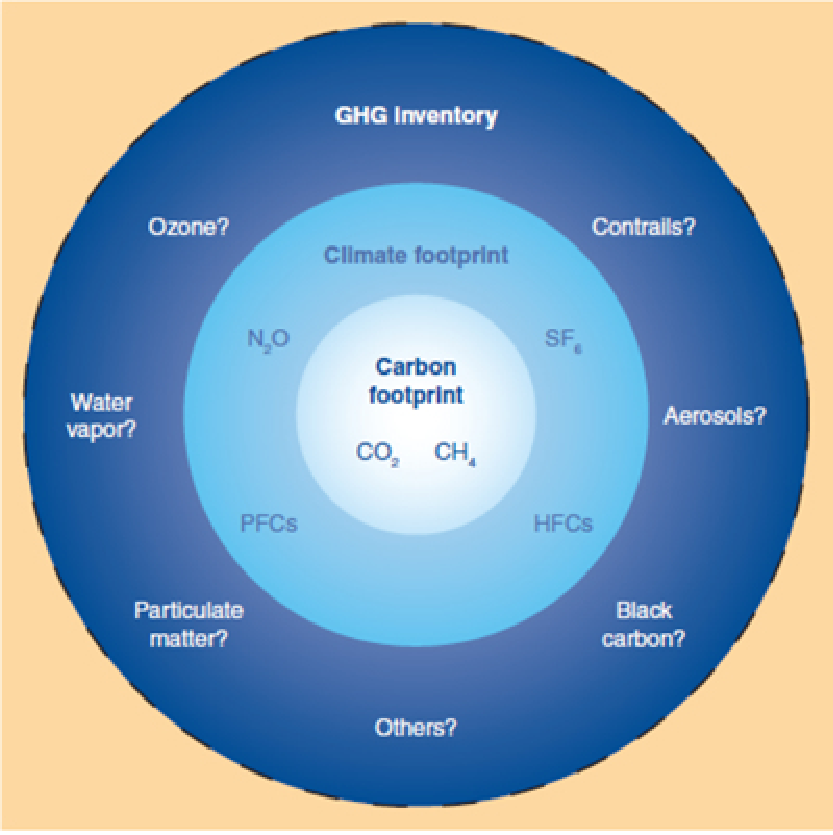
\includegraphics{./Figures/figure16.pdf}
		\rule{35em}{0.5pt}
	\caption[Carbon Emissions Measures]{Three measures for carbon emissions\cite{reference23}}
	\label{fig:ghgEmissionMeasures}
\end{figure}

\subsection{Calculating carbon emissions}

The process of calculating carbon footprints is relatively straightforward and consists of the following steps.

\begin{enumerate}
  \item
        Initially, all emission sources for the subject need to be compiled and classified; for example, an emission source for an individual might be his daily travels to work with bus.
  \item
        A method for quantifying the emissions of each source has to be selected. The unit for that quantity is expressed in CO2e, which combines CO2 and CO4 emissions.
  \item
        All the data that are needed by the method have to be gathered; for example, a method might need some activity data\cite{reference25} and an appropriate conversion factor (or emission factor); we will come back to these terms in a bit.
  \item
        A documentation of the method is vital, so that computed values can be validated by re-executing the same method, in the future. Provenance, which we discussed in previous sections, can be a good solution.
\end{enumerate}


\subsection{Gathering Emissions Sources}

The carbon footprint calculation process starts by gathering the emissions sources for the subject. To better identify possible emissions sources we can distinguish two types of emissions: direct and indirect emissions.

Direct are the emissions which the subject has full control of. These are the emissions that are primarily produced during the combustion of fossil fuels. On the other hand, indirect emissions are not directly associated with a specific activity, but are due to the demand for products brought by the subject in question; for example, each product that we buy consists of a number of activities that result in the product being on super-markets shelves. Apparently, all these activities cause CO2e emissions. This implies that our demand for products indirectly produced a quantity of CO2e that was emitted to the environment.

\subsection{Classifying Emissions}
The prime reason that lies behind the decision for categorizing emissions is the problem of double counting. In essence, it refers to the problem of associating the same quantity of carbon emissions to multiple subjects\cite{reference23:25}. To avoid this issue, emissions are classified into three distinct scopes.

\begin{description}
  \item[Scope 1]
        In scope 1, the direct carbon emissions of individuals, activities or systems can be found; for example, carbon emissions produced by a car owned by a company.
  \item[Scope 2]
        Scope 2 consists of emissions that are produced from energy generation. It basically, refers to energy purchased by the subject in question, for own consumption.
  \item[Scope 3]
        Emissions which are the result of the subject's actions that take place outside the organization or geographic boundaries are scope 3 emissions. In general, this sort of emissions are said to be shared by several subjects rather solely belong to one.
\end{description}


\subsection{Calculation Methods}

The next step in calculating emissions is to select an appropriate calculation method, based on the data that are available. The simplest formula suggests that the number of units of the activity that occurred be multiplied by an appropriate conversion factor (emission factor\cite{reference25}. To better illustrate this concept, imagine that the carbon emissions of a trip made by car needs to be calculated. In that case, we can multiply the distance traveled (or fuel consumed) by a value that defines the CO2e emissions of that car per kilometer units.

According to the accuracy and quality of the data that are present, calculation methods can be classified into three categories or tiers; if we choose to use the fuel consumed by a car then several factors that determine the quality of this figure should be considered. The type of the journey, the vehicles age and condition are some of the factors that affect the quantity of fuel consumption. A tier Three method will consider all those factors, as it will use the actual quantity of the fuel used. Further, it will multiply this number by an emission factor published by a government body and which is associated with the particular fuel type. A tier Two method will be less accurate. It will take the distance traveled as the main activity data and multiply it by the emissions factor for the specific car model. Finally, a tier One method will yield the least accurate figure, because it will use the least specific data. In particular, an average distance (published by some government's authority) for that sort of cars will be multiplied by the emission factor associated with that fuel type.

\subsection{HEI Scope 3 Carbon Emissions}

In this section we will briefly describe how higher educational institutions (HEI) should calculate scope 3 carbon emissions caused by travels made by the institution's members\cite{reference24}. First we will remind that scope 3 emissions are those that are caused by sources that are not owned by the HEI. A representative example would be, emissions that are produces by commuting travels by a transport mean that is not owned by the HEI e.g. bus, train etc.

There are two categories of travels: business and commuter travels. The main factor that determines the scope of carbon emissions is the mode of transport that was used; for instance, emissions caused by transport means owned by the HEI are scope 1 emissions. However, travels are often made by modes of transport owned by third-party bodies; hence the corresponding emissions are regarded as scope 3 emissions.

\begin{figure}[htbp]
	\centering
		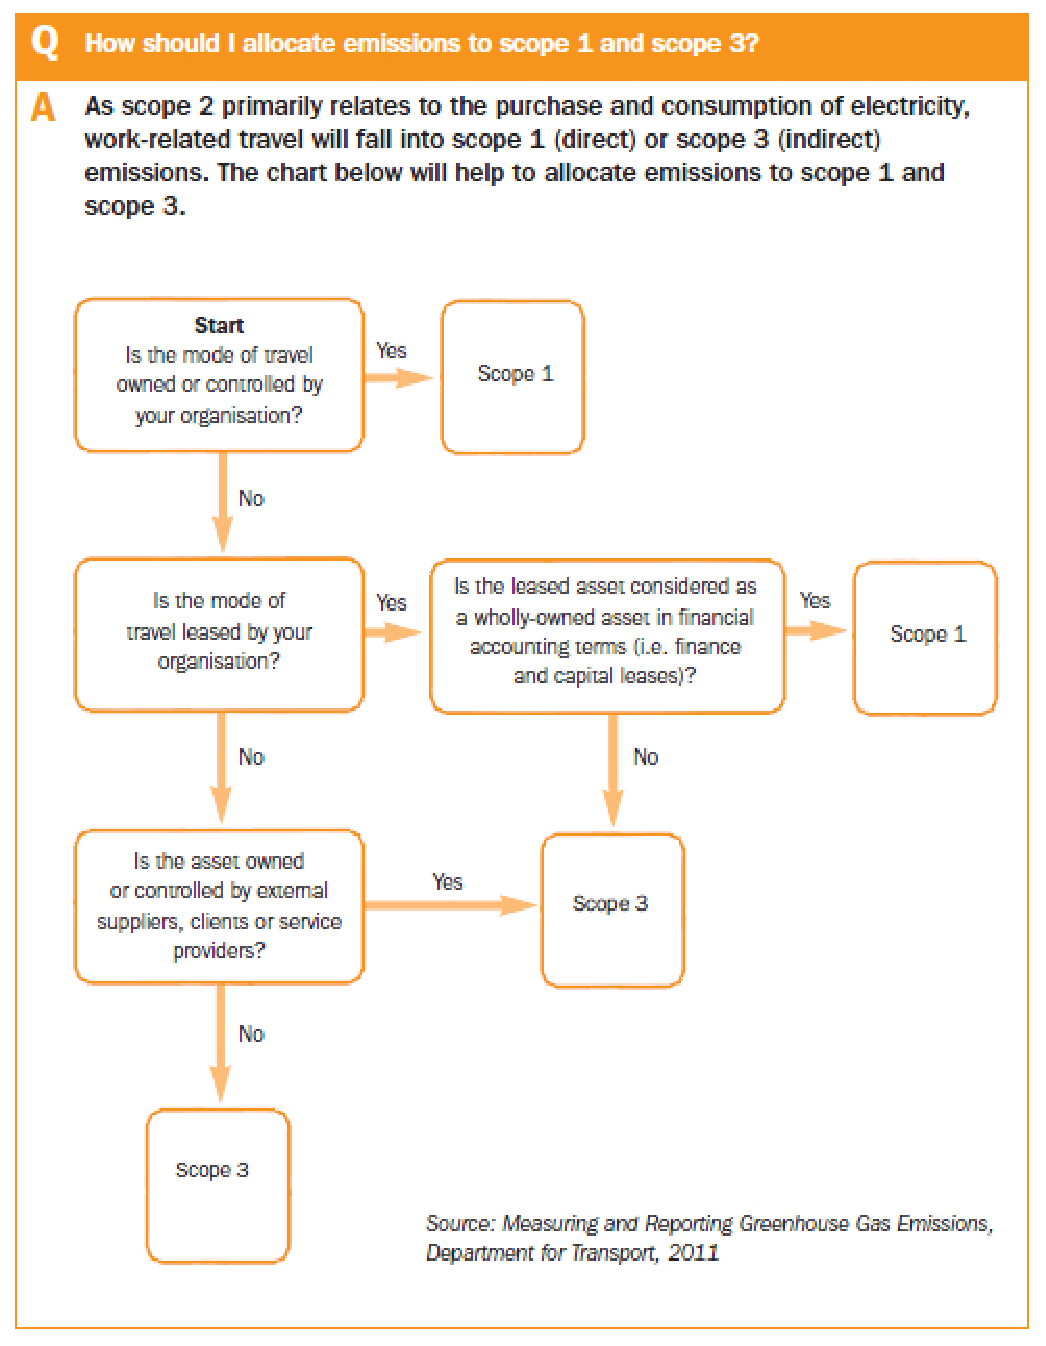
\includegraphics[scale=0.85]{./Figures/chapter2/figure17.pdf}
		\rule{35em}{0.5pt}
	\caption[Seperating Scope 1 and Scope 3 Emissions]{How to distinguish scope 1 and scope 3 emissions\cite{reference24}}
	\label{fig:scope1Scope3}
\end{figure}


\subsection{Travel emissions calculation}

The process of calculating emissions caused by travels is the same with what we have presented earlier. As far as travels are concerned, the type of transport mean determines the emission factor that will be used in the calculation formula.

\section{Carbon Footprint Applications}

In this section we will present some of apps that are similar to the one we have developed, in that they calculate individual carbon footprints. The pros and cons of each are highlighted.

\subsection{CarbonFootPrint.com}

This is an online carbon emissions calculator. The tool is hosted on the www.carbonfootprint.com web site\footnote{\url{http://www.carbonfootprint.com/calculator.aspx}}.
Users can insert some data concerning their household activities (e.g. kWh of electricity consumed), as well as, the distance they have traveled by various mode of transport; for instance, figure \ref{fig:carbonFootprintCom} shows the form for adding the distance traveled by a car.

\begin{figure}[htbp]
	\centering
		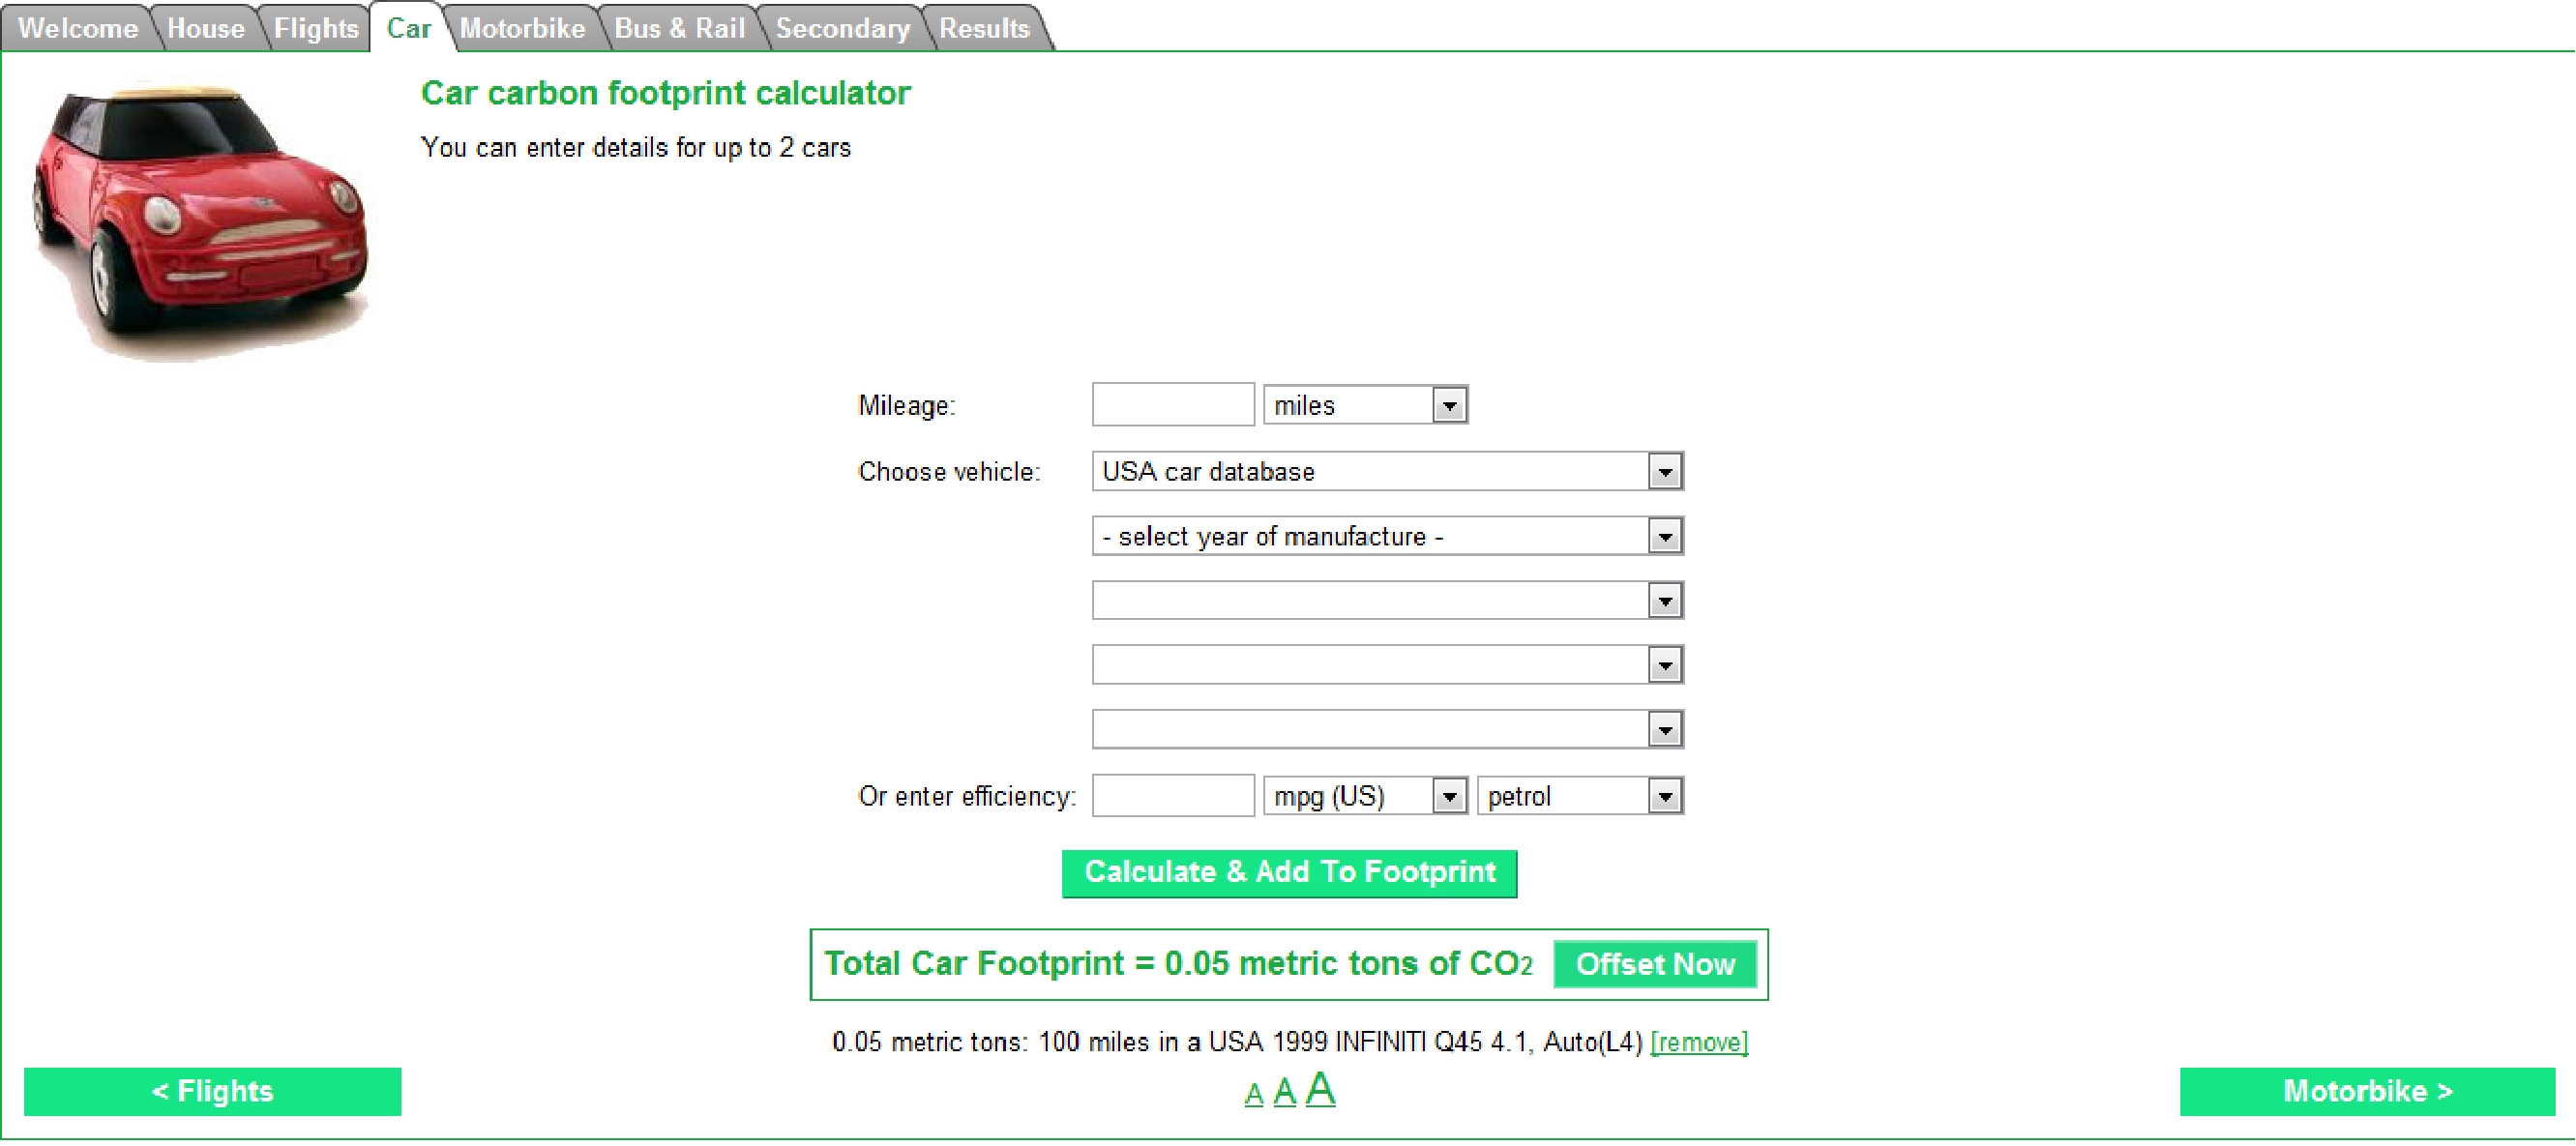
\includegraphics[scale=0.30]{./Figures/chapter2/figure18.pdf}
		\rule{35em}{0.5pt}
	\caption[Form for adding travels made by a car]{Form for adding travels made by a car}
	\label{fig:carbonFootprintCom}
\end{figure}

The tool summarizes all the carbon emissions via a web UI, where carbon footprints of individuals are presented.

\begin{figure}[htbp]
	\centering
		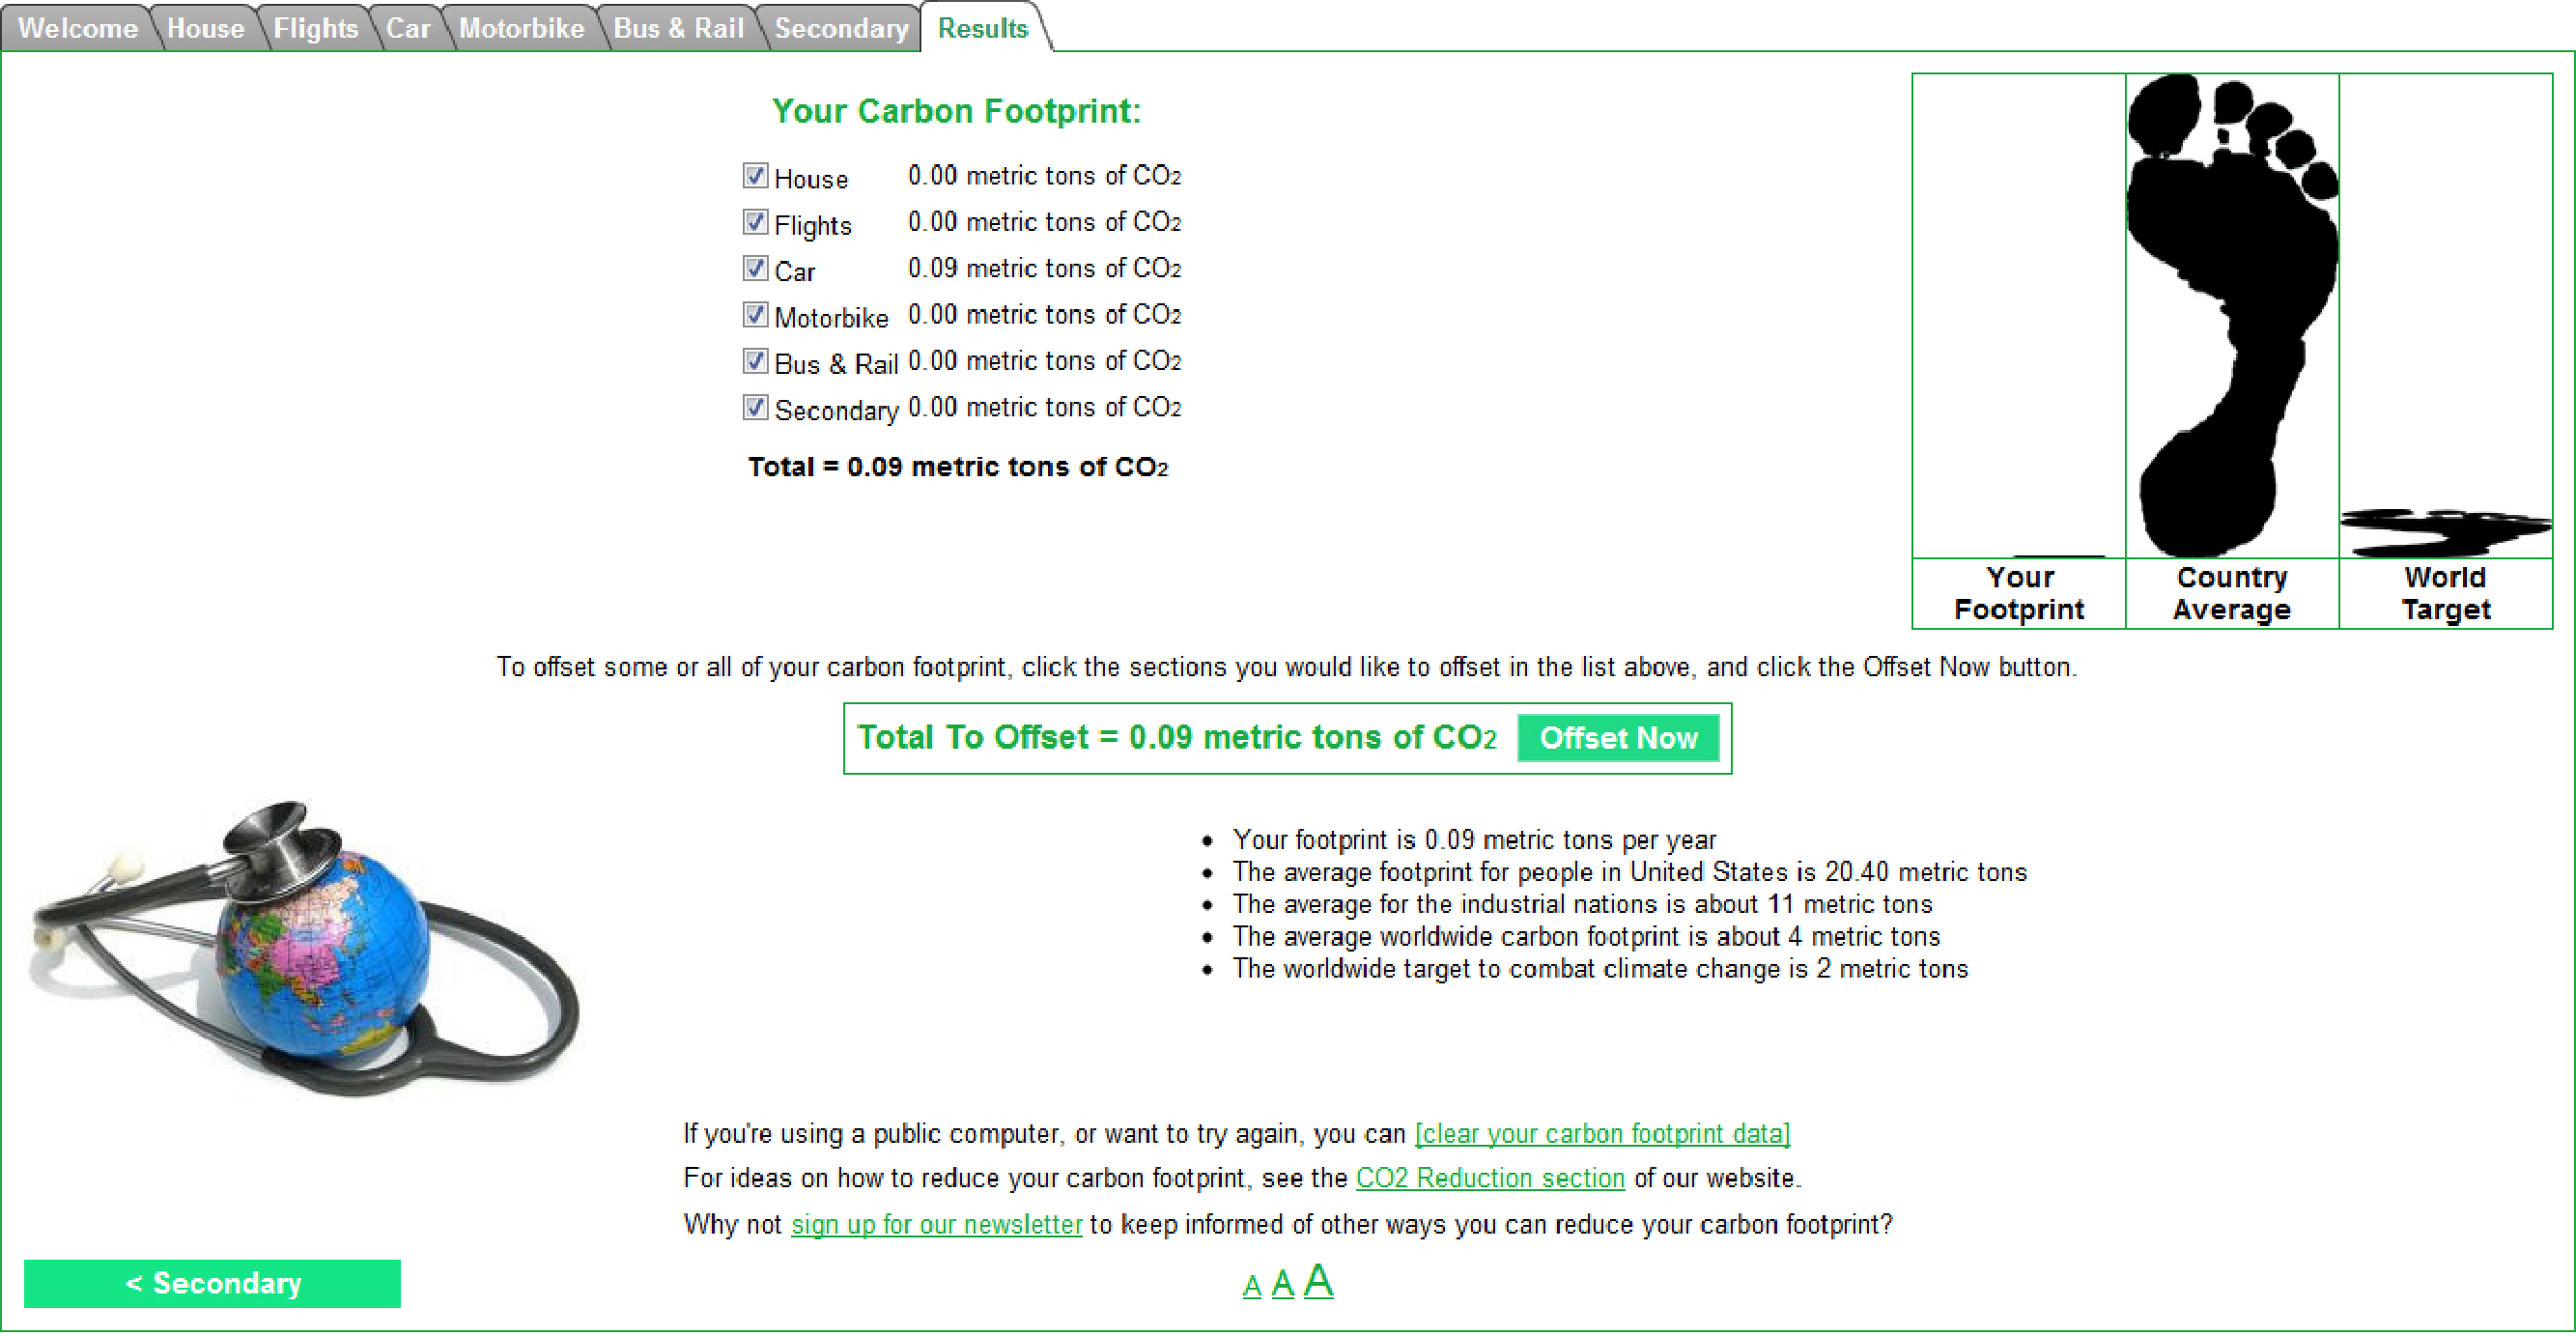
\includegraphics[scale=0.30]{./Figures/chapter2/figure19.pdf}
		\rule{35em}{0.5pt}
	\caption[Carbon footprint report]{Carbon footprint report}
	\label{fig:carbonFootprintCom2}
\end{figure}

A factor that might hinder users from tracking their carbon footprints is the knowledge of traveled distance. It is obvious that such information is difficult to be possessed or can be erroneously inserted.

\subsection{AMEE Location Footprinter}

A slightly more usable tool is provided by AMEE\footnote{\url{http://www.amee.com/}} and is called AMEE Location Footprinter\footnote{\url{http://alf.ameeapps.com/}}. It is a web based tool that operates in conjunction with Foursquare\footnote{\url{https://foursquare.com/}}. The biggest advantage of the app is that it does not require users to insert any data. It, essentially, reads all the check-ins the user make on Foursquare, finds the distance between those check-ins and tries to identify the transport that was used. Ultimately, it computes the carbon emissions caused by those journeys and sends an email enclosing user's carbon footprint report, on a weekly basis.

The main downside is that it calculates the carbon emissions caused by journeys from one check-in to another. In other words, if users have to constantly make check-ins on Foursquare such that an accurate carbon footprint can be computed. Furthermore, as mentioned earlier, the application makes a guess about the transport mean used between check-ins. That means that the guess might be wrong in which case the computed carbon emissions value is not accurate and misleading.

\begin{figure}[htbp]
	\centering
		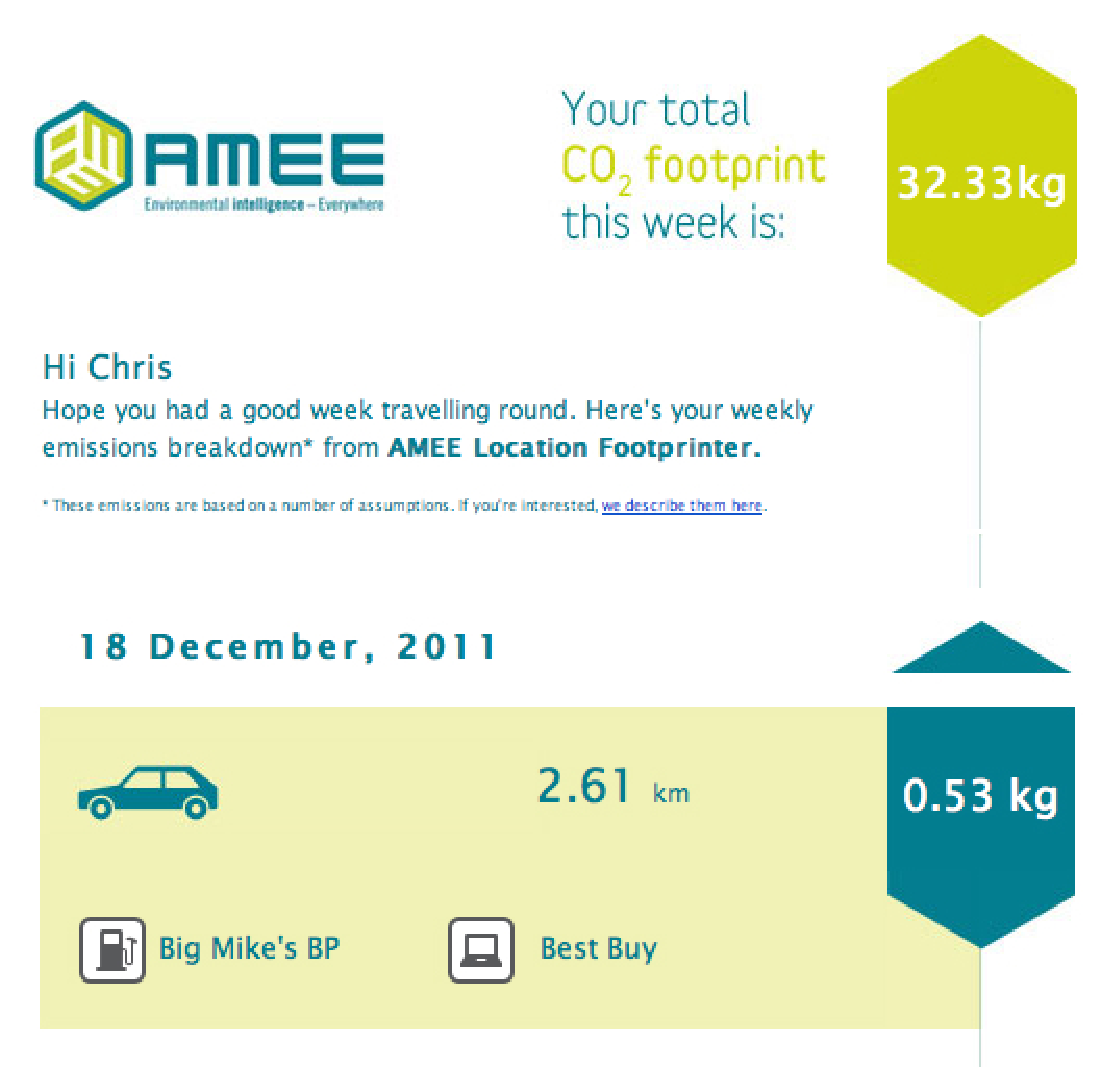
\includegraphics[scale=0.70]{./Figures/chapter2/figure20.pdf}
		\rule{35em}{0.5pt}
	\caption[Carbon footprint report send to user's email]{Carbon footprint report send to user's email}
	\label{fig:ameeLocationFootprinter}
\end{figure}


\subsection{Ecobot}

Ecobot\footnote{\url{http://ecobot.taxi.ca/}} is a free open-source application that calculates the amount of power, fuel and paper you consume during the course of a day. Users are free from adding nay data to the app. It makes a guess about how frequently you travel by tracking wireless network you access. Additionally, it records the amount of papers you use for printing and the energy consumed by several household appliances like computer, video games and televisions.

\begin{figure}[htbp]
	\centering
		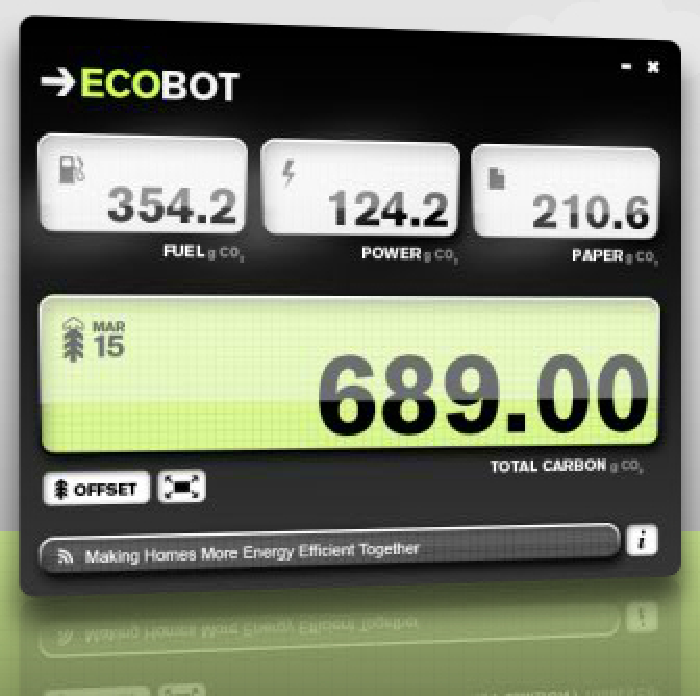
\includegraphics[scale=0.80]{./Figures/chapter2/figure21.pdf}
		\rule{35em}{0.5pt}
	\caption[Ecobot carbon footprint calculator]{Ecobot carbon footprint calculator}
	\label{fig:ecobot}
\end{figure}

The application makes several speculations to figure out the activities undertaken by the user. Thus, the total carbon emissions it calculates might be far from the actual amount that user emits. Another disadvantage is that it is currently compatible only with Mac OS.

\subsection{The Guardian's Quick Carbon Calculator}

The official Guardian's web site offer a carbon footprint calculator\footnote{\url{http://www.guardian.co.uk/environment/interactive/2009/oct/20/guardian-quick-carbon-calculator}}, which computes carbon emissions caused by home activities, travels and shopping habits.

\begin{figure}[htbp]
	\centering
		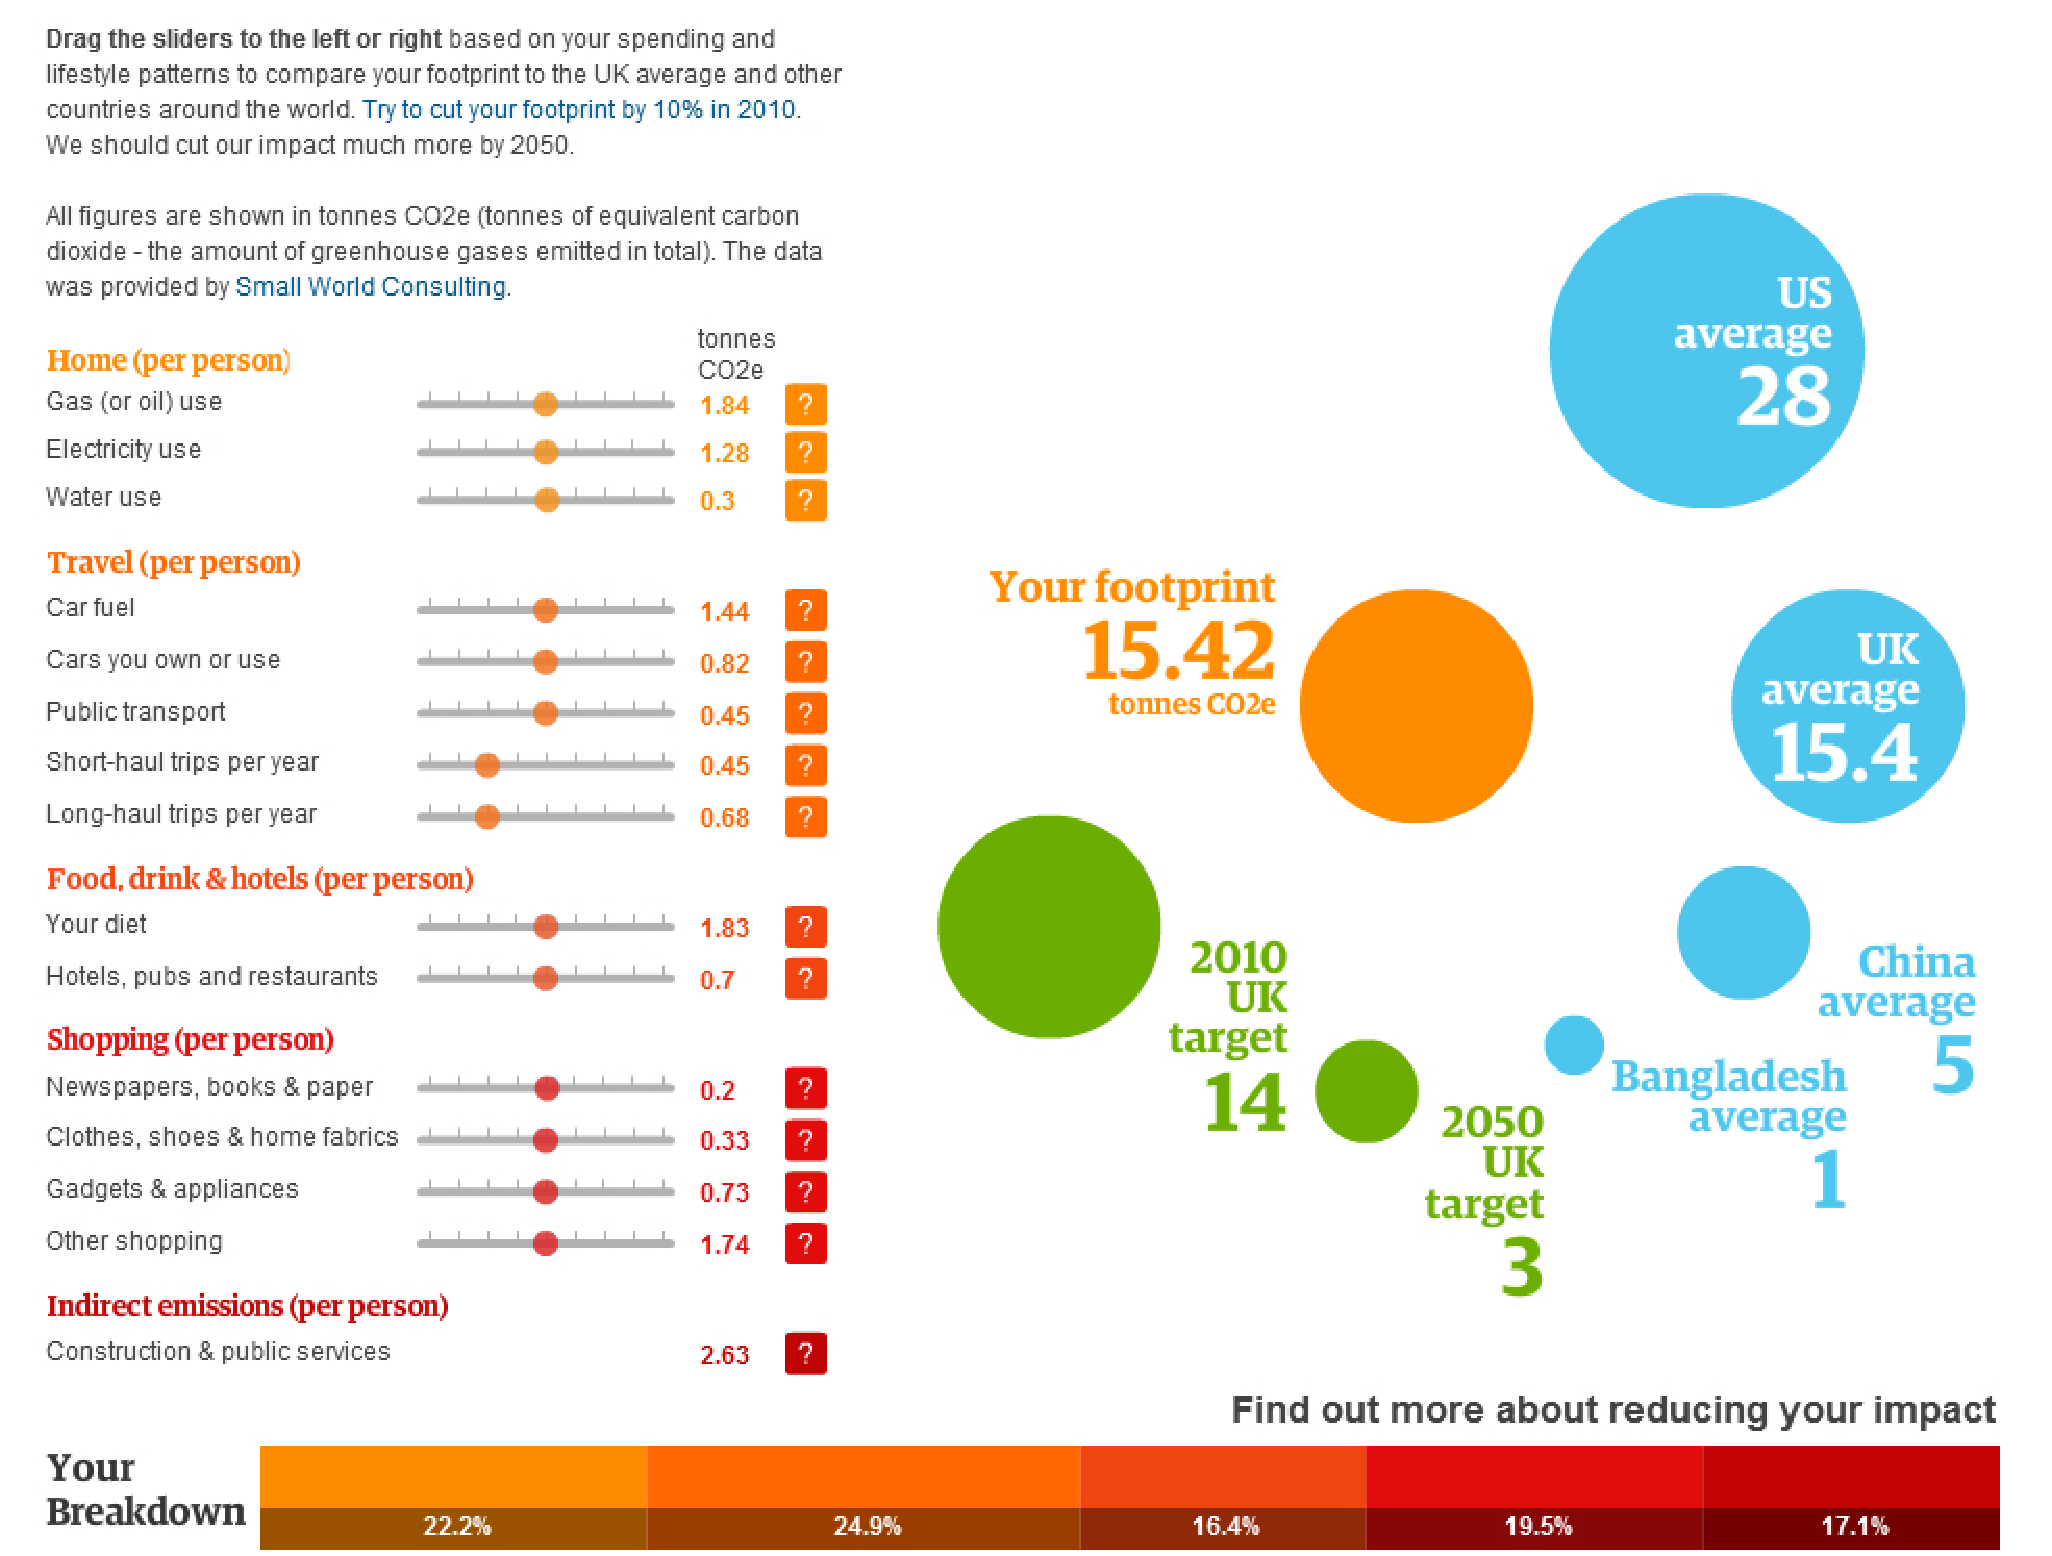
\includegraphics[scale=0.35]{./Figures/chapter2/figure22.pdf}
		\rule{35em}{0.5pt}
	\caption[The Guardian's quick carbon calculator]{The Guardian's quick carbon calculator}
	\label{fig:guardiansCarbonCalculator}
\end{figure}

You can add the money you spend for various products and the application calculates a rough estimation of carbon emissions of the corresponding activities. An advantage of that app is that the input data come in the form of money spent; therefore it is easy for users to insert accurate values. On the other hand, the computed carbon emissions might not be accurate, due to abstract description of activities added by users; for instance, users specify the cars they own, but they do not clarify the exact model of those cars.

\subsection{Other Applications}

Table 2.1 summarizes several other tools that have been developed for calculating carbon footprints.

\begin{table}
  \centering
  \begin{tabular}{|p{100px}|p{100px}|p{100px}|p{100px}|}
    \hline
    Name & Developer & Compatibility & Available \\
    \hline
    CarbonTrack & Logo Design and Marketing Ltd & IOS & YES \\
    Zero Carbon & Mobitelio LTDA & IOS & YES \\
    Clear Standards' Carbon Tracker & Don Frehulfer & IOS & YES \\
    Carbon Diem & Andreas Zachariah & BlackBerry & NO \\
    Ecorio & Ecorio, Inc. & Android & YES \\
    Carbon Footprint Calculator & 1WebApps.com & IOS & YES \\
    ecoFootprint & Max Gontar & Android & YES \\
    MyPlanet & Blue Chip Marketing Worldwide & Android & YES \\
    \hline
  \end{tabular}
  \caption{List of applications}\label{carbonCalculators}
\end{table}

\section{Tools and Libraries}

In this section we will present the tools that were user throughout each step of this project. A brief description of each tool will be given accompanied by the rationale for using it.

\subsection{Tools Used for Literature Research}

Table 2.2 summarizes the tools that were used for the literature research phase of the project.

\begin{table}
  \centering
  \begin{tabular}{|p{100px}|p{100px}|p{100px}|p{100px}|}
    \hline
    Tool  & Description & Usage & License \\
    \hline
    Mendeley Desktop & Mendeley is desktop application for managing references and organizing your research.& Mendeley was primarily used for searching and storing scientific papers. & EULA \\ \hline

    Evernote & A software for taking notes in different format, such as text notes, web pages, images etc. & Mendeley Evernote was used in two different ways. It was the main tool for keeping notes concerning the project. Additionally, a web clipper plugin was used to capture useful information from various web sites. & Freemium \\ \hline

    LaTeX & A markup language for composing different kinds of documents. & Latex was used in conjunction with the WinEdt editor for writing the project report. & LaTeX Project Public License (LPPL) \\ \hline

    Adobe Fireworks CS6 & Adobe software for processing vector graphics. It is extensively used by web developers for creating web site prototypes.  & The software was used for creating and processing the images added to the report and the web application. & Shareware \\ \hline

    \hline
  \end{tabular}
  \caption{List of tools used for literature research}\label{literatureTools}
\end{table}


\subsection{Tools Used During the Application's Design Phase}

Table 2.3 summarizes the tools that were used for during the application's design phase of the project.

\begin{table}
  \centering
  \begin{tabular}{|p{100px}|p{100px}|p{100px}|p{100px}|}
    \hline
    Tool  & Description & Usage & License \\
    \hline
    Visual Paradigm for UML 10 & Visual paradigm offers an integrated environment for capturing requirements for software development,  UML modeling, data modeling and many other features that simplify the design of software. & The tool was used for UML and data modeling. & Proprietary with Free Community Edition \\ \hline

    Microsoft Visio & An application for drawing different sort of diagrams. Part of the Microsoft office suite. & Visio was used for drawing the system architecture as well as provenance graphs. & Proprietary commercial software \\ \hline

    Balsamiq Mockups & Balsamiq mockups is a tool for quickly creating mock-ups for the application's UI. & The tool was used to draw low-fi sketch wireframes.  & Proprietary commercial software \\ \hline

    Axure RP Pro 6.5 & A prototyping and wireframing tool for designing prototypes for web applications. A feature for generating interactive HTML pages is provided.  & Axure was used during the design phase to create a rapid prototype of the applications UI. & Proprietary commercial software \\ \hline

    Microsoft Project 6.5 & A project management tool provided by Microsoft. The tool is useful for scheduling and managing tasks of large and small projects.  & The application was used for scheduling and managing the tasks needed for the project completion, with the aid of Gantt charts. & EULA \\ \hline

    \hline
  \end{tabular}
  \caption{List of tools used during the application's design phase}\label{designTools}
\end{table}

\subsection{Tools Used During Application's Implementation Phase}

Table 2.4 summarizes the tools that were used for during the application's implementation phase of the project.

\begin{table}
  \centering
  \begin{tabular}{|p{100px}|p{100px}|p{100px}|p{100px}|}
    \hline
    Tool  & Description & Usage & License \\
    \hline
    PostgreSQL & An object relational database management system (ORDBMS) & PostgreSQL was the used to persist data produced by the web application. & PostgreSQL license \\ \hline

    Aptana Studio 3 & Aptana studio is an integrated development environment (IDE) used for creating software applications. It is designed for web application development & Aptana studio was the IDE used for developing the web application. & Dual License Aptana Public License, v1.0 GNU General Public License \\ \hline

    Fiddler2 & Fiddler is a tool used for debugging http requests/responses. It, essentially, acts as a proxy server capturing HTTP traffic. & The tool was used primarily for debugging http GET and Post request made via AJAX calls in the web application.  & Freeware (LPPL) \\ \hline

    Github & A well-known web-based application using the Git revision control system for tracking changes in the source code of an application.  & Github was the revision control system that was used during the application development. & Freemium \\
    \hline
  \end{tabular}
  \caption{List of tools used during the application's implementation phase}\label{implementaioTools}
\end{table}

\subsection{Frameworks and Libraries used during the application's implementation phase}

Table 2.5 summarizes various frameworks and libraries that were used during the application's implementation phase.


\begin{longtable}{|p{100px}|p{100px}|p{100px}|p{100px}|}
    \hline
    Tool  & Description & Usage & License \\
    \hline
    Django & An open-source web application framework for developing web 2.0 applications. The framework is written in Python and follows the Model View Controller architectural pattern. & Django was the framework that used to develop our web application. & BSD License \\ \hline

    Ember.js & Ember.js (ex SproutCore) is a relatively new JavaScript framework for applying Model View Controller pattern. Some of the powerful features offered are UI binding (MVVM pattern), computed properties, observable properties, auto-updating templates and many more. & The framework was used to organize the client side code, and apply separation of concerns. Features like UI bindings were utilized for enriching the application's user interactivity. & MIT License \\ \hline

    Handelbars.js & A JavaScript template engine for composing updatable and easily manageable html templates.  & Handlelbars.js was used in conjunction with ember.js to leverage all the capabilities offered by the framework.  & MIT License \\ \hline

    Kendo UI (web) & A powerful JavaScript library with lots of capabilities pertaining to web application UI design and rich user interactions.  & We used several HTML widgets like calendars, tab menus etc. to enrich the appearance and user interaction of the application. & GPL v3 \\
    \hline

    jQuery & Probably the most popular JavaScript library used today. It extends the core capabilities of the language and simplifies several tasks to minimize the boilerplate code. & jQuery was extensively used in the application to accomplish tasks like, AJAX request, JSON request etc. & MIT license or GNU GPL \\
    \hline

    Bing Maps API & Bing is widely known web search engine provided by Microsoft. Among others it includes a mapping service called Bing Maps, which can be leveraged by application via an API. & Bing maps API was used to simplify the task for users of inserting addresses. & Various Licensing options \\
    \hline

    Highcharts & A JavaScript charting library for drawing different kinds of charts (e.g. line, alpine, area charts etc.). & The library was used for drawing the charts that are presented to users on the carbon footprint report page & Free for non-commercial \\
    \hline

    JavaScript Infovis Toolkit & A powerful visualization library written in JavaScript. & The provenance graphs that are displayed on the carbon emission report page were implemented with the aid of this library. & New BSD License \\
    \hline

    jQuery.validate & An open-source JavaScript library for manipulating date through JavaScript code. & The library was used for different tasks concerning date manipulation (e.g. converting datetime formats, locating the amount of days passed etc.). & MIT License \\
    \hline

    jQuery.vTicker & A jQuery plugin for vertical news scrolling. & The library was used to support the news RSS widget on the home page. & Free (details not specified) \\
    \hline

    jQuery.zrssfeed & A jQuery plugin that reed RSS feeds from any web resource using the Google Feeds API. & The library was used to read RSS feeds from the ECS department of the University of Southampton. & Free \\
    \hline

    Date.js & A plugin library for jQuery for html form validation & The library was used for validating  user inputs (via html forms) & MIT License \\
    \hline

    Provpy & A python library developed at the university of Southampton for creating and storing provenance information.  & All the provenance tasks were achieved via this library. & Free \\
    \hline

    Matplotlib & A python plotting library capable of creating a big diversity of plot figures  & Static provenance graphs in PNG format were produced with the aid of this library.  & Matplotlib License \\
    \hline

    Googlemaps  & A python library which supports features like, geo decoding, driving directions, local search and reverse geo decoding via Google maps API. & The library was used to calculate the driving distance between two addresses.  & Affero GNU Public License , GNU Library or "Lesser" General Public License version 3.0 (LGPLv3) \\
    \hline

    Twitter bootstrap  & A widely used framework for designing layout for HTML pages and applying pretty CSS styles. & The application's layout and styling was configured with the help of this framework. & Apache License 2.0 \\
    \hline

  \caption{List of framework and libraries used during the application's implementation phase}\label{implementaioFrameworks}
\end{longtable}



\section{Summary}
This chapter was an intro to the theory of provenance and carbon footprinting. Some core principles of provenance of electronic data were initially presented along with a description of different ways for representing, storing and fetching provenance information. We then introduced some fundamental notions of carbon footprinting. Finally, we discussed about a set of applications which are similar to the one we developed; pros and cons of each applications were given.
 % Background Theory

%% Chapter 3

\chapter{Application Design} % Write in your own chapter title
\label{Application Design}
\lhead{Chapter 3. \emph{Application Design}} % Write in your own chapter title to set the page header

\section{introduction}

In chapter 2 we investigated the theory and technology underpinning the design and developments of our application. In this chapter we investigate the design phase. We will primarily focus on some low level aspects of the design phase by presenting various UML diagrams.

\section{Application's Design Phase}

\subsection{System Requirements}

The application design started by investigating the system requirements. In this section we summarize the initial requirements of the system and provide the use cases derived from those requirements.

Figure \ref{fig:sysRequirementsDiagram} illustrated an abstract view of the requirements.

\begin{figure}[htbp]
	\centering
		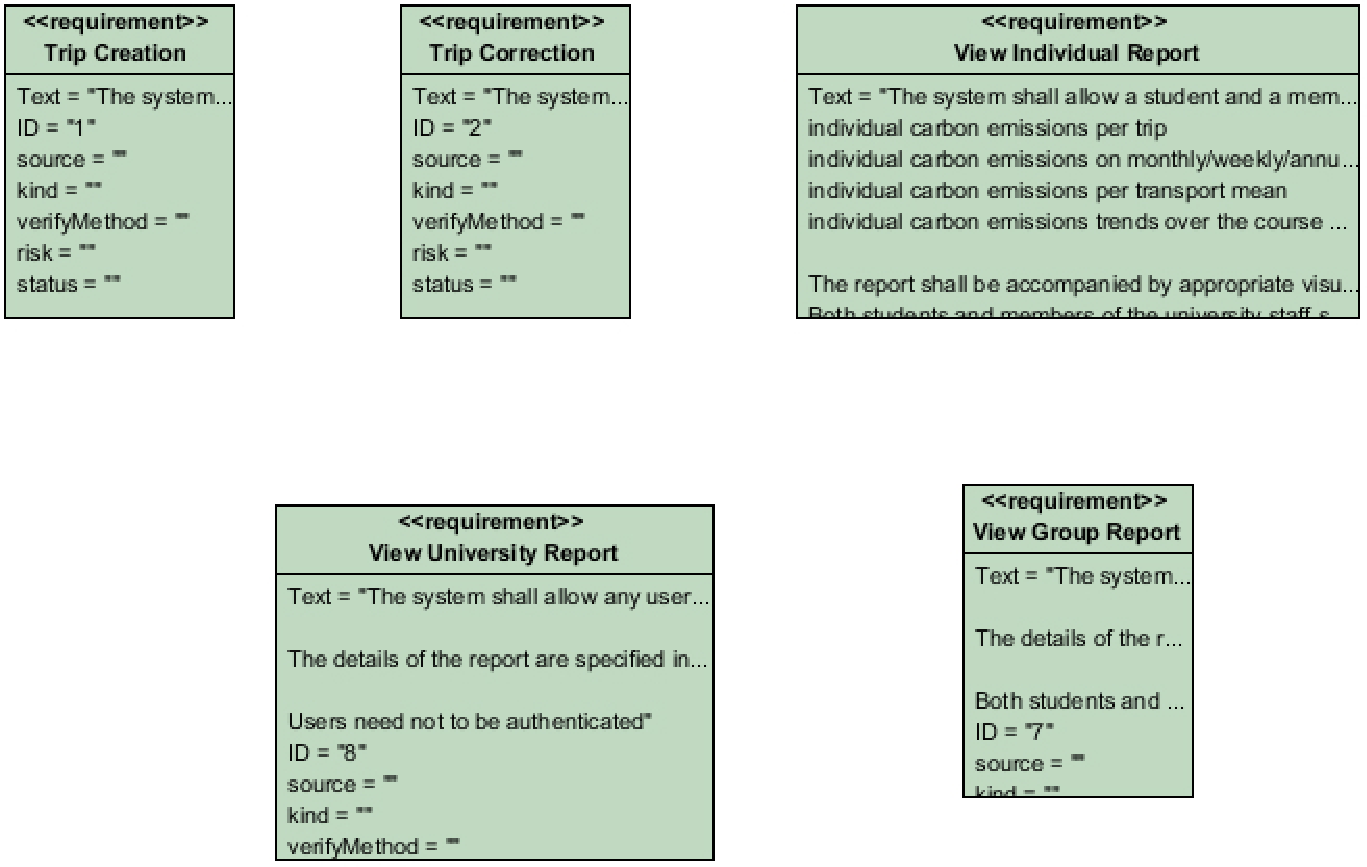
\includegraphics[scale=0.60]{./Figures/chapter4/figure1.pdf}
		\rule{35em}{0.5pt}
	\caption[System requirements diagram]{System requirements diagram}
	\label{fig:sysRequirementsDiagram}
\end{figure}

Expanding on the diagram depicted in figure \ref{fig:sysRequirementsDiagram} we can view the following requirements.

\begin{description}
  \item[Trip Creation : Requirement]
        The system shall allow a student or a member of the staff to add a new trip, by providing the appropriate information, such as, source and destination of the trip, as well as, the transport mean that was used. A user must be authenticated before adding a new trip.
  \item[Trip Correction : Requirement]
        The system shall allow a student or a member of the university staff to edit a trip that he has already created. This action demands users to be authenticated.
  \item[ View Individual Report : Requirement]
        The system shall allow a student and a member of the university staff to view his individual report presenting his carbon footprints. The report shall present:

        \begin{enumerate}
          \item individual carbon emissions per trip
          \item individual carbon emissions on monthly/weekly/annual basis
          \item individual carbon emissions per transport mean
          \item individual carbon emissions trends over the course of time
        \end{enumerate}

        The report shall be accompanied by appropriate visualization elements (e.g. charts etc.).
  \item[View Group Report : Requirement]
        The system should allow a student and a member of the university staff to view carbon emission report, concerning the groups that they are member of (e.g. research groups etc.).
        Both students and members of the university have to be authenticated.
  \item[View University Report : Requirement]
        The system shall allow any user to view a summary report about the carbon emissions of the entire university.
        Users need not to be authenticated.
\end{description}


\subsection{Use Cases}

Finding the requirements was the first step. The next step is to fing use cases of the application. Figure \ref{fig:useCasesDiagram} illustrates a diagram with the system's use cases. A description of each use case is summarized in table \ref{useCases} further below along with the corresponding flow of events.

\begin{figure}[htbp]
	\centering
		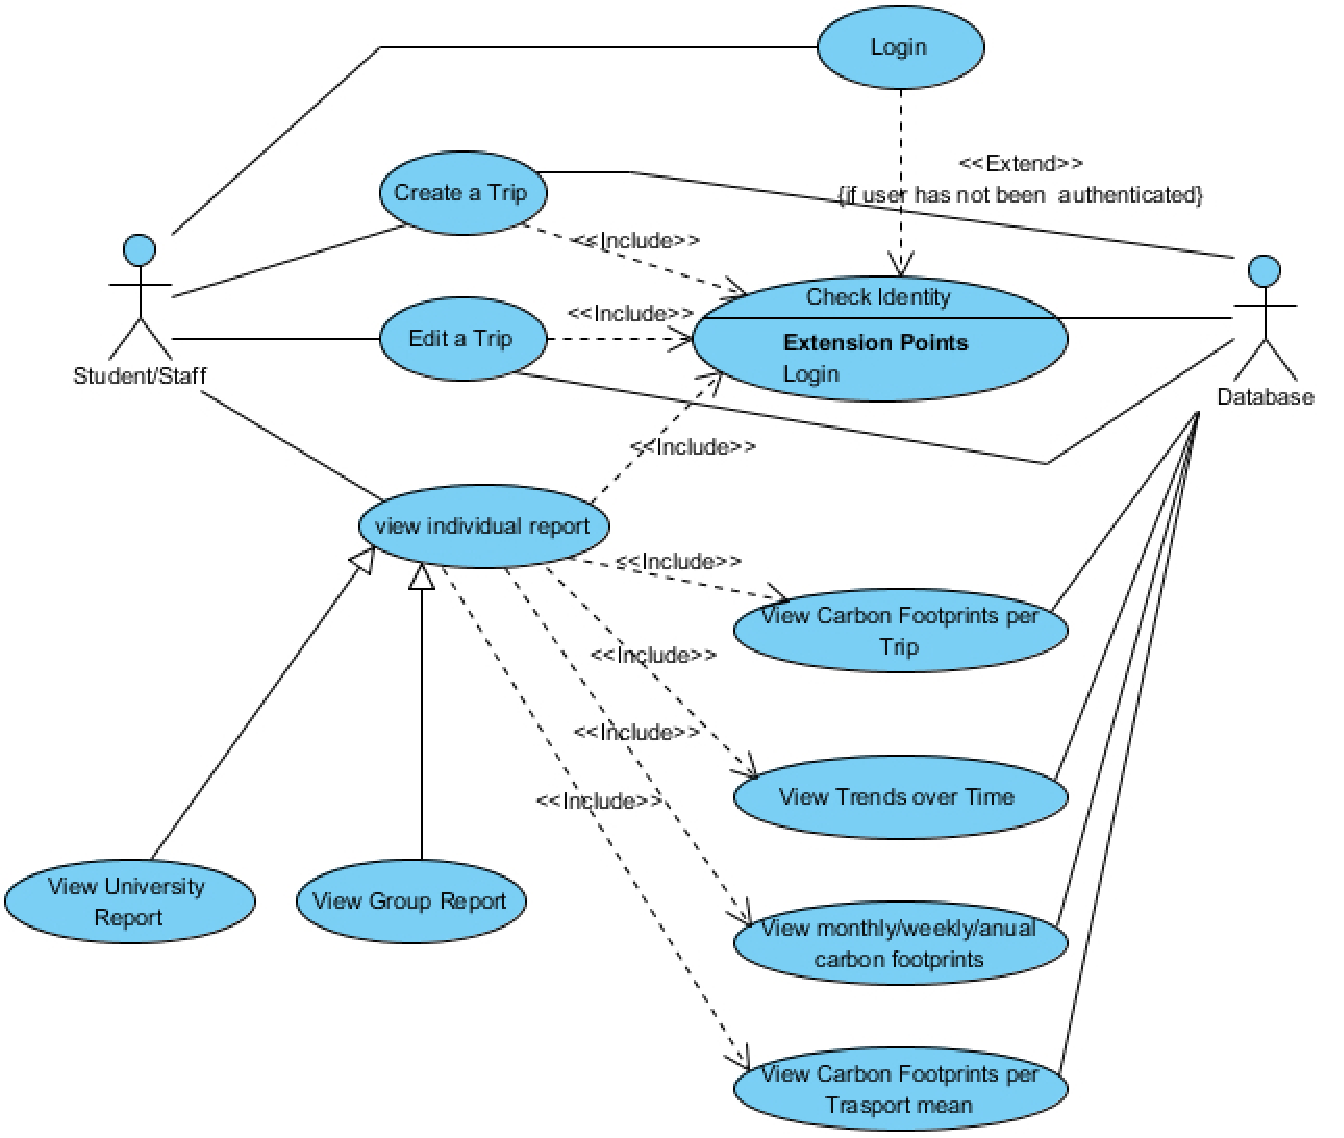
\includegraphics[scale=0.60]{./Figures/chapter4/figure2.pdf}
		\rule{35em}{0.5pt}
	\caption[Use cases diagram]{Use cases diagram}
	\label{fig:useCasesDiagram}
\end{figure}

\begin{description}
  \item[Student/Staff : Actor]
        Students or members of university staff.
  \item[Database : Actor]
        The persistent storage where all the data are stored.
  \item[Create a Trip : Use Case]
        A use case where authenticated users can add trips they made, by providing the appropriate details.
  \item[Check Identity : Use Case]
        A process that assures that specific operations can only be executed by authenticated users.
  \item[Edit a Trip : Use Case]
        A use case indicating that an authenticated user (i.e. a student or a member of the staff) can modify the details of a trip that she has added to the system.
  \item[Login : Use Case]
        A use case where users provide their credentials in order to enter the system and are able to execute operations that require them to be authenticated (e.g. trip creation).
  \item[view individual report : Use Case]
        A use case where authenticated users (i.e. students or members of the university staff) can view their individual carbon emissions report trough a rich web UI.
  \item[View Carbon Footprints per Trip : Use Case]
        A use case where authenticated users (e.g. students and members of university staff) can view the carbon emitted by each of the trips they have made.
  \item[View monthly/weekly/anual carbon footprints : Use Case]
        A use case where authenticated users (e.g. students and members of university staff) can view the carbon emissions caused by their travel activities, on weekly, daily or annual basis.
  \item[View Trends over Time : Use Case]
        A use case where authenticated users (e.g. students and members of university staff) can view their carbon emissions over the course of time, through appropriate web UI widgets (e.g charts).
  \item[View Carbon Footprints per Trasport mean : Use Case]
        A use case where authenticated users (e.g. students and members of university staff) can view the carbon emissions categorized by the transport means that were used.
  \item[View Group Report : Use Case]
        A use case where authenticated users can view the carbon emissions report for the groups that they are members of.
  \item[View University Report : Use Case]
    	A use case where any user can view carbon emissions report about a university.
\end{description}



\subsubsection{Flow of Events}

Each use case comprise a number of actions that needs to be executed. We therefore, strived to locate those steps way before the implementation part was started. We provide the flow of events for our use cases, in the following lines.

\paragraph{Create a Trip : Use Case}
\mbox{}\\
\newline
\textcolor[rgb]{0.00,0.00,1.00}{\textbf{Steps}}

\begin{verbatim}
1.  The user asks the system to create a new trip
2.  Check Identity
3.  The system asks the user to add the source and destination of the trip,
    as well as, the transport mean that was used. For each of those fields,
    the system might let the user to choose from some pre-defined values
    (e.g. common addresses and transport means) that had been configured
    by the user.
4. The user provides all the required information and submits the form.
    4.1. The user adds the source and destination address of the trip
        4.1.1. if The address exist in the system
            4.1.1.1. if the user wants to select a private address
                    (i.e. addresses had bee added by the user in the past)
                4.1.1.1.1. The user selects an address from the list of private
                           addresses
                4.1.1.1.2. The system shows the address on a map
                4.1.1.1.3. The user confirms the address or picks a different
            4.1.1.2. else
                4.1.1.2.1. The user selects an address from the list of public
                           addresses
                4.1.1.2.2. The system shows the address on a map
                4.1.1.2.3. The user confirms the address or picks a different
                     end if
        4.1.2. else
            4.1.2.1. The users chooses to add a new address
            4.1.2.2. The system shows the address creation form
            4.1.2.3. The user enters the address
            4.1.2.4. The user specifies the visibility of the address
                    (i.e. private or public)
            4.1.2.5. The user click the add address button
            4.1.2.6. The system stores the address into the persistent storage
               end if
    4.2. The user adds the transport mean
        4.2.1. The user selects the type of the transport mean
              (e.g. car, bus, taxi etc.)
        4.2.2. if the user selected the car option
            4.2.2.1. if the user wants to select one of the cars he stored into
                     the system
                4.2.2.1.1. the system show all the cars that the user stored in
                     the system
                4.2.2.1.2. the user selects a car
            4.2.2.2. else
                4.2.2.2.1. The system show a car creation form
                4.2.2.2.2. The user adds some the information about the car
                           (e.g. engine capacity,name etc. )
                4.2.2.2.3. The system add the car to the list of cars that have
                           been used by the user
                     end if
        4.2.3. else
            4.2.3.1. The user selects the specific type of transport mean
               end if
5. The user add the date and time of the trip
6. A new trip is created and inserted into the persistent storage.
\end{verbatim}


\paragraph{Edit a Trip : Use Case}

\mbox{}\\
\newline
\textcolor[rgb]{0.00,0.00,1.00}{\textbf{Steps}}

\begin{verbatim}
1. The user asks the system to edit a trip
2. Check Identity
3. The system retrieves from the persistent storage, the the trips that
   has been added by the user. Trips should be easily searchable, so that
   users can easily locate the one they want to alter.
4. The user selects the trip she wants to modify
5. The system presents a form populated with the details about the
   selected trip.
6. The user modifies the trip details and submits the form
7. The modified trip record is stored back to the persistent storage
\end{verbatim}

\paragraph{Login : Use Case}

\mbox{}\\
\newline
\textcolor[rgb]{0.00,0.00,1.00}{\textbf{Steps}}

\begin{verbatim}
1. while User is not authenticated
    1.1. The systems asks the user to provide with her credentials
    1.2. The user enters her credential
    1.3. The system checks if the given data exist in the database
    1.4. The system authenticates the user
   end while
\end{verbatim}

\textcolor[rgb]{0.00,0.00,1.00}{\textbf{Extension}}
\begin{verbatim}
1.3.a. Authentication Failure
    1. The system cannot find user's credential in the database
    2. An error message is displayed
    3. jump to 1.1. The systems asks the user to provide with her credentials
\end{verbatim}

\paragraph{Check Identity : Use Case}

\mbox{}\\
\newline
\textcolor[rgb]{0.00,0.00,1.00}{\textbf{Steps}}

\begin{verbatim}
1. The system checks if the given user has already been authenticated
2. The system allow the user to execute the operations that need
   authentication
\end{verbatim}

\textcolor[rgb]{0.00,0.00,1.00}{\textbf{Extension}}
\begin{verbatim}
1.a. Login
\end{verbatim}


\paragraph{View individual report : Use Case}

\mbox{}\\
\newline
\textcolor[rgb]{0.00,0.00,1.00}{\textbf{Steps}}

\begin{verbatim}
1. The user asks the system to view her individual carbon emissions report
2. Check Identity
3. The system presents the individual report for the user
    3.1. View Carbon Footprints per Trip View monthly/weekly/anual carbon
    footprints View Trends over Time View Carbon Footprints per Trasport mean
\end{verbatim}


\subsubsection{Activity Diagrams}

The flow of events for each use case that we oulined earlier, can be better illustrated with the aid of UML Activity Diagrams that follows.

\begin{figure}[htbp]
	\centering
		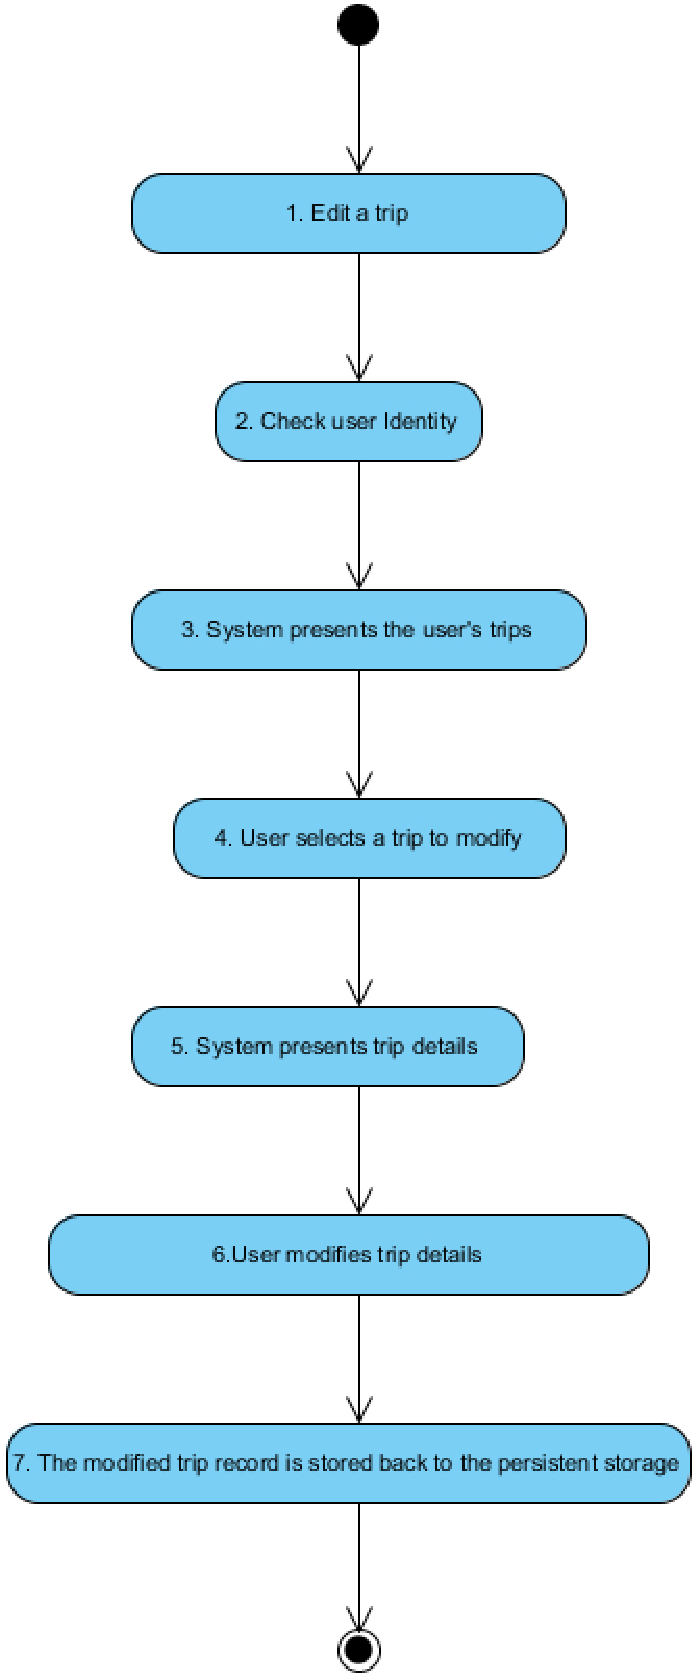
\includegraphics[scale=0.80]{./Figures/chapter4/figure3.pdf}
		\rule{35em}{0.5pt}
	\caption[Edit trip activity diagram]{Edit trip activity diagram}
	\label{fig:activityDiagramEditTrip}
\end{figure}


\begin{figure}[htbp]
	\centering
		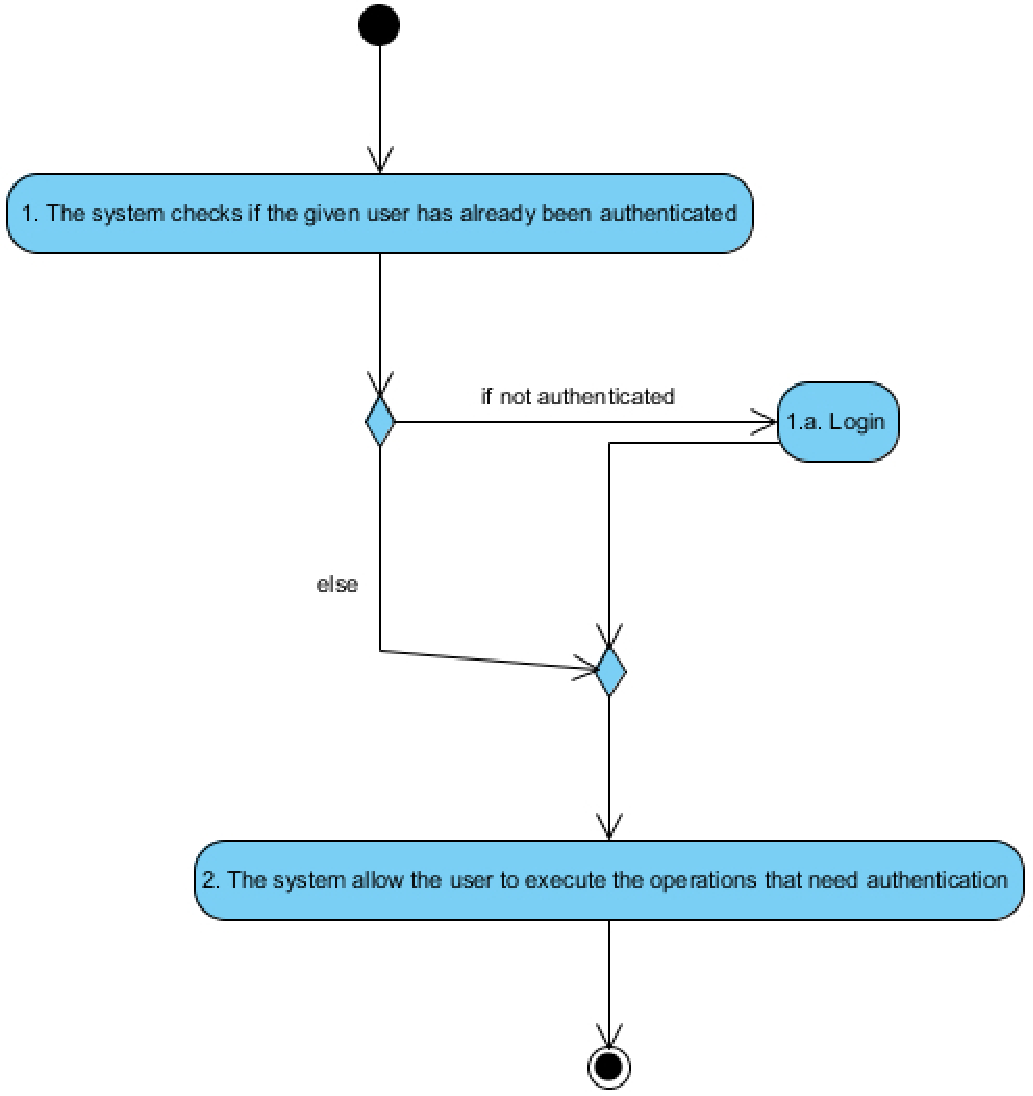
\includegraphics[scale=0.80]{./Figures/chapter4/figure4.pdf}
		\rule{35em}{0.5pt}
	\caption[Check identity activity diagram]{Check identity activity diagram}
	\label{fig:activityDiagramCheckIdentity}
\end{figure}

\begin{figure}[htbp]
	\centering
		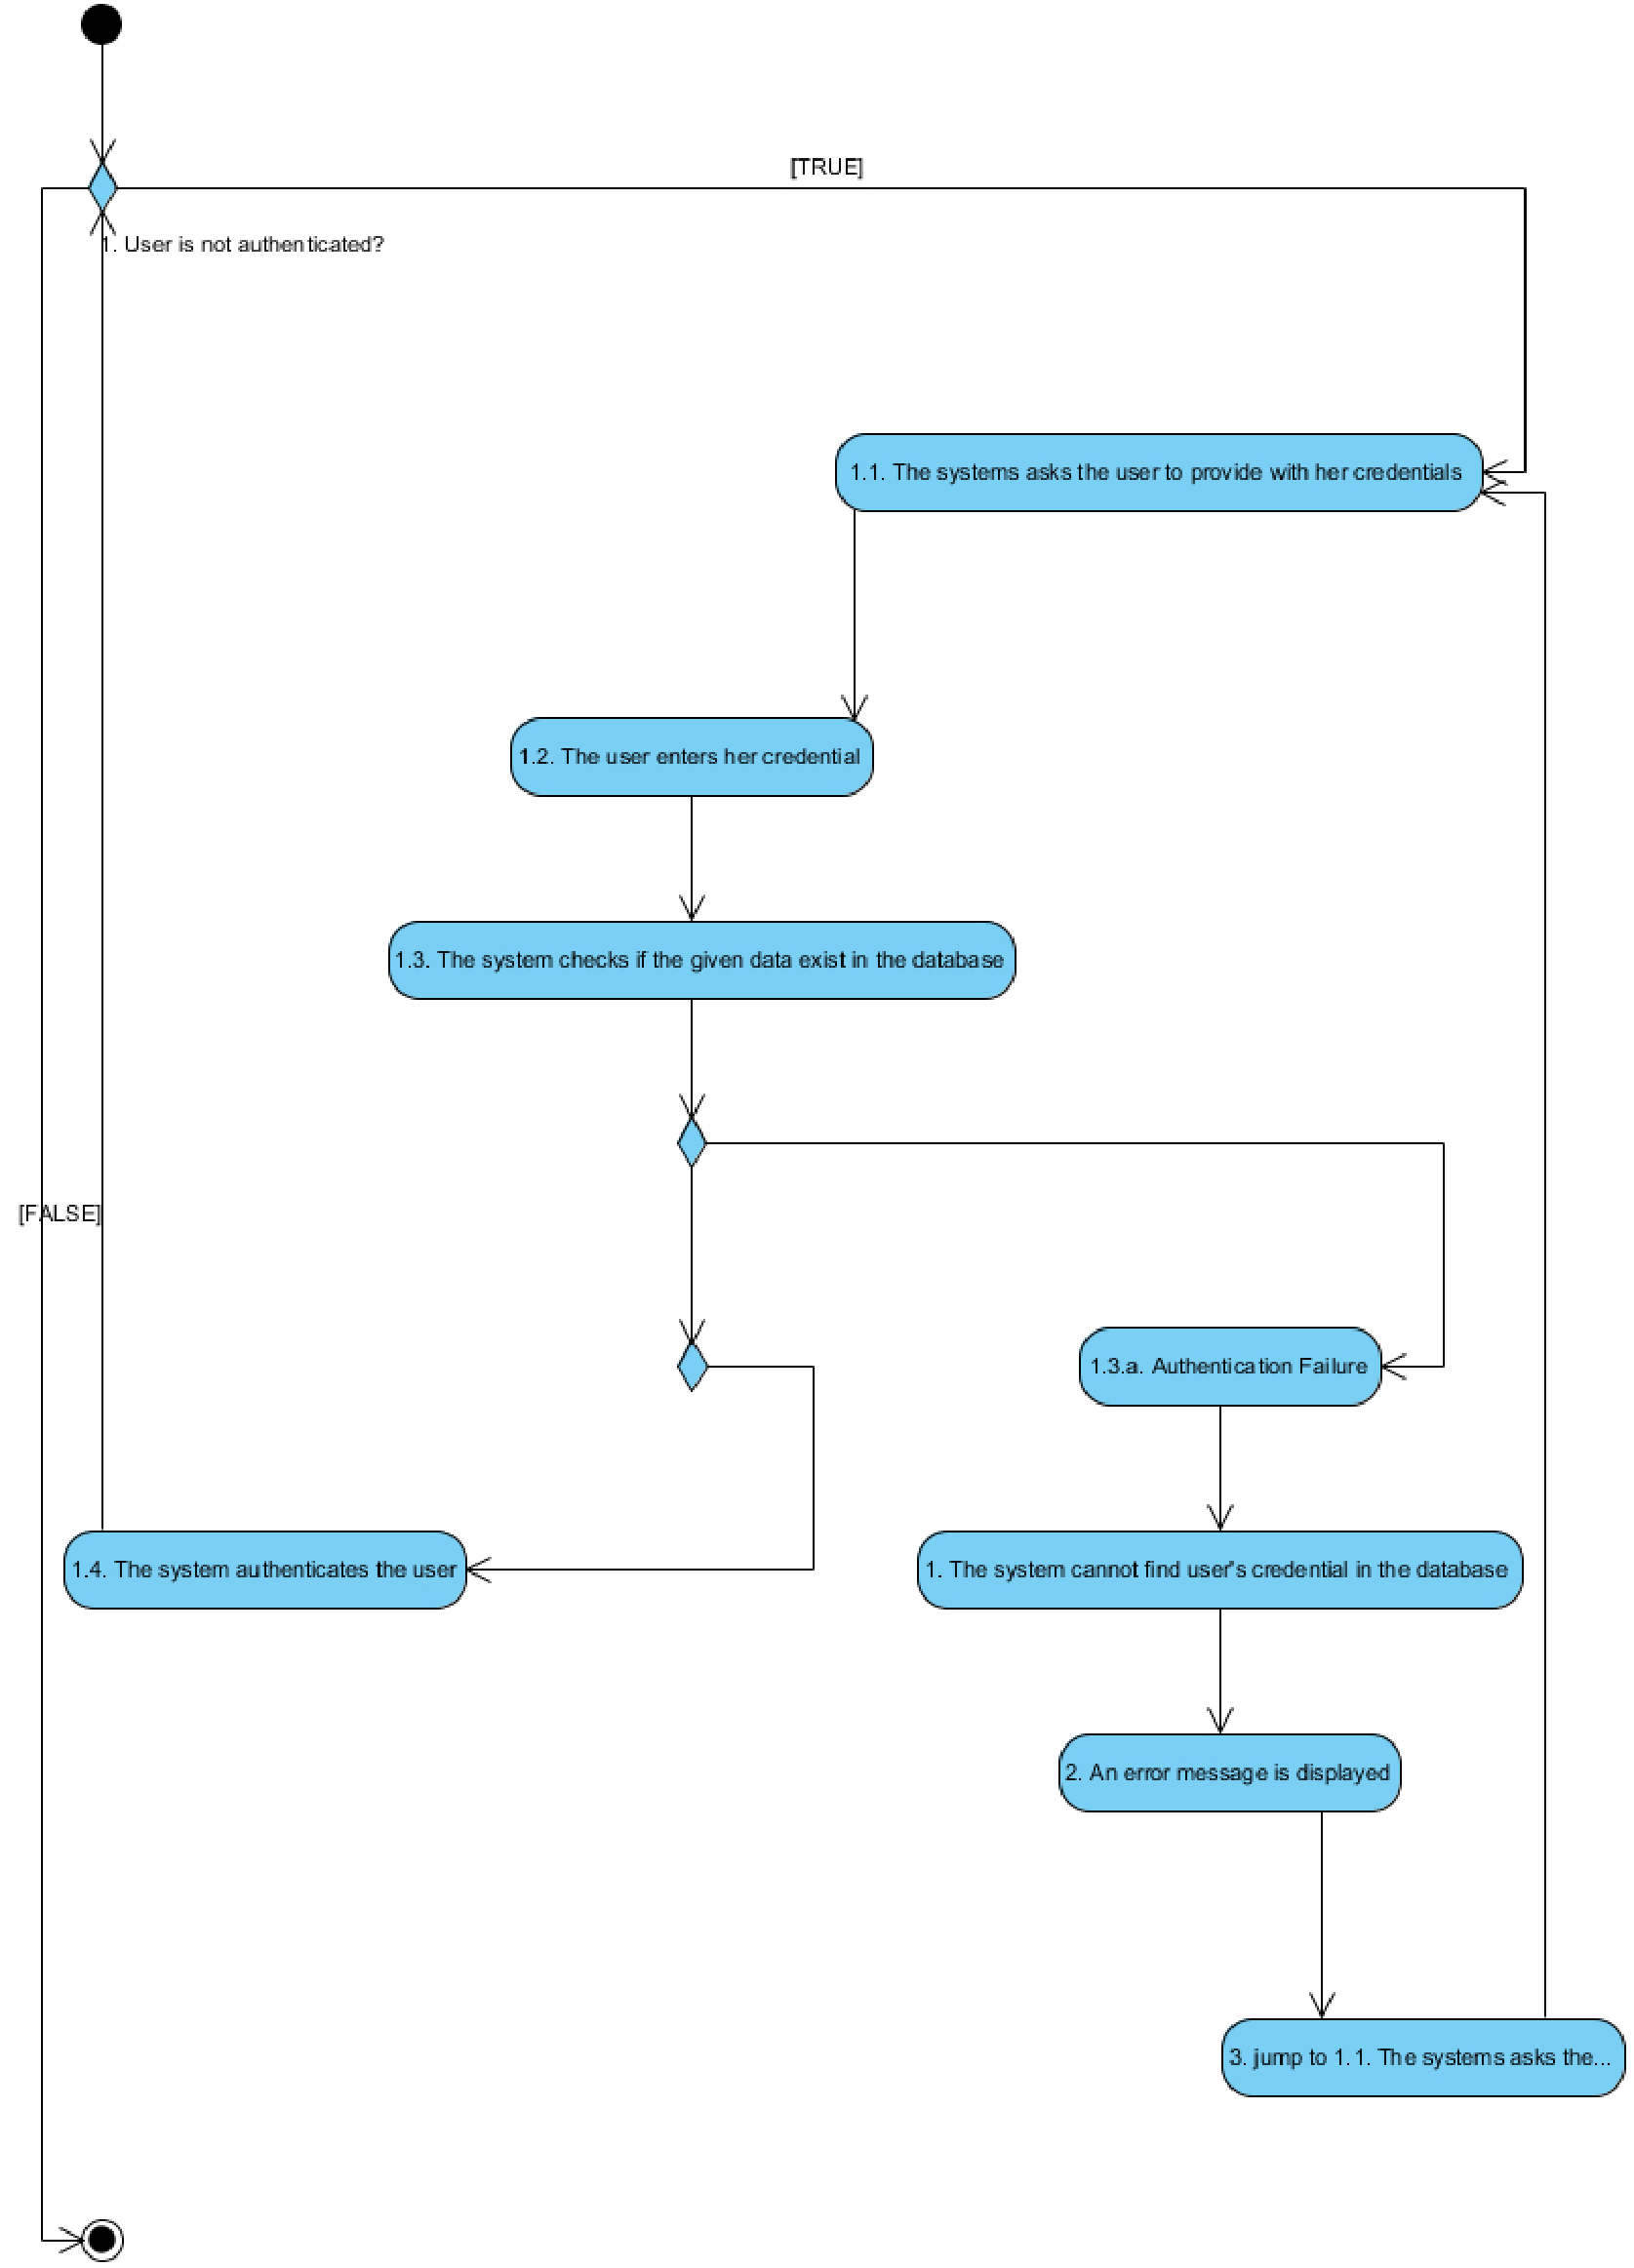
\includegraphics[scale=0.50]{./Figures/chapter4/figure5.pdf}
		\rule{35em}{0.5pt}
	\caption[Login activity diagram]{Login activity diagram}
	\label{fig:activityDiagramLogin}
\end{figure}


\subsection{Class Diagrams}

The code of the application both on back-end and front-end was written in object oriented languages (though javascript is not pure object oriented language); therefore, what follows are class diagrams for the back and front-end.

\subsubsection{Back End}

Figure \ref{fig:backEndClassDiagram} shows the back end class diagram and table \ref{backEndClasses} summarizes brief descriptions for each class.

\begin{figure}[htbp]
	\centering
		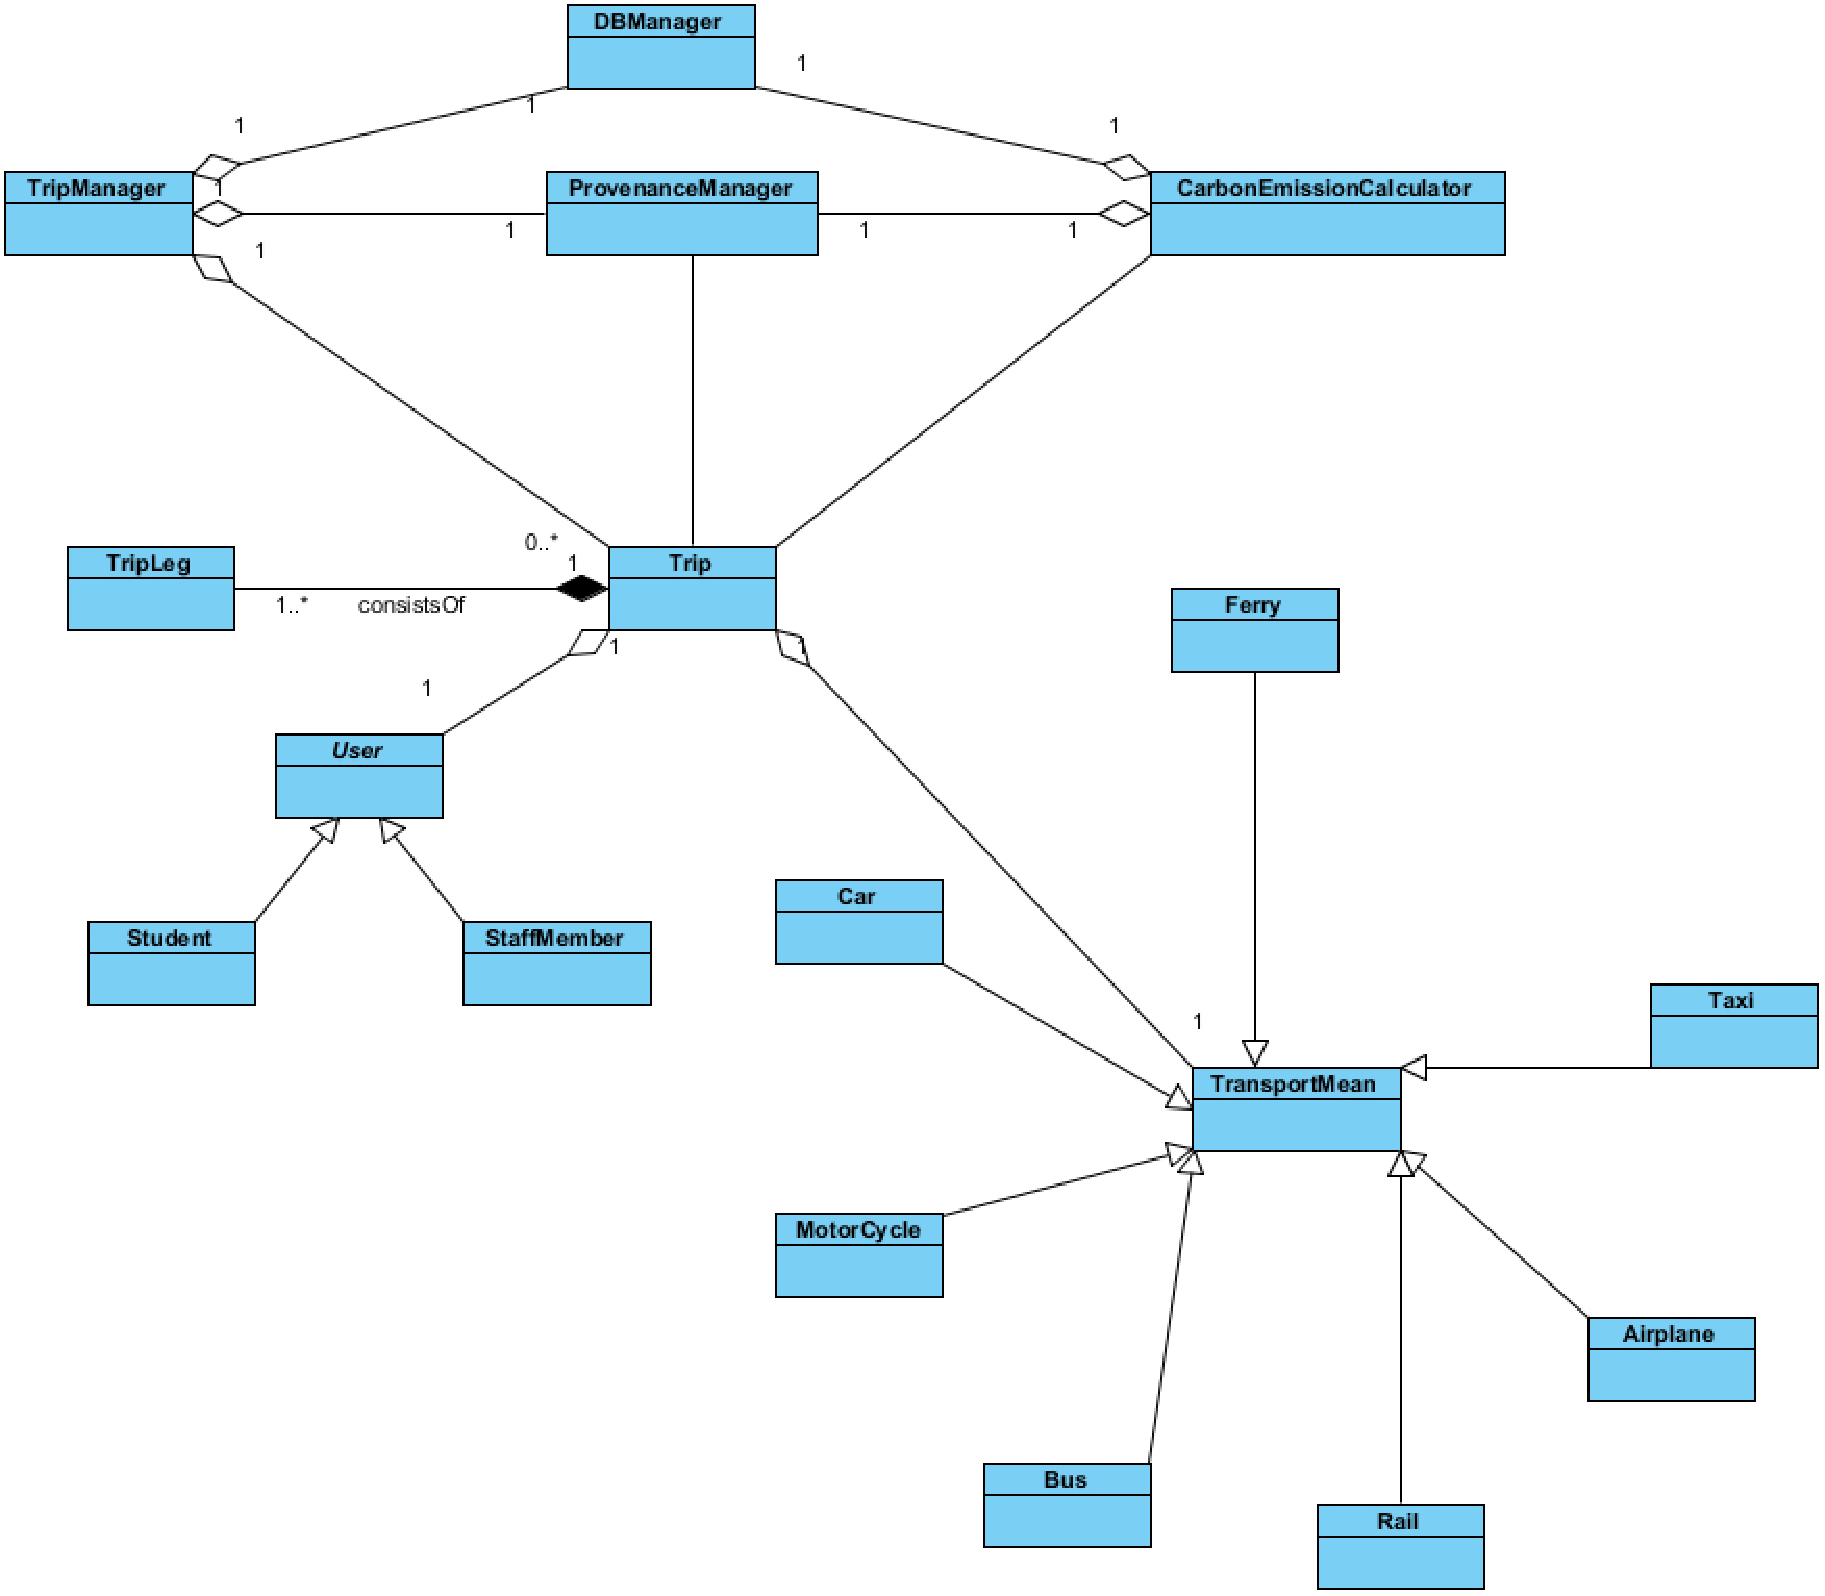
\includegraphics[scale=0.50]{./Figures/chapter4/figure6.pdf}
		\rule{35em}{0.5pt}
	\caption[Back-end class diagram]{Back-end class diagram}
	\label{fig:backEndClassDiagram}
\end{figure}

\begin{table}
  \centering
  \begin{tabular}{|p{150px}|p{250px}|}
    \hline
    Class  & Description\\
    \hline
    Trip & The main enity of the application. It represents the trip that users make. \\
    TripLeg & Each trip can have several intermediary step. Trip legs represents those steps \\
    TransportMean & The class represents transport means that are used during user's trips. It is an abstract class which has concrete subclasses (i.e Car, Motorcycle etc.) \\
    User & instances of this class refer to the user of our application. \\
    TripManager & A class responsible for all the tasks concerning user trips management, such as trip addition, trip modification etc. \\
    ProvenanceManager & A class responsible for provenance-related tasks, such as creation, storing etc. of provenance graphs. \\
    CarbonEmissionCalculator & A class responsible for calculating the carbon emissions of trips, trip legs etc. \\
    DBManager & A class responsible for database-related tasks. To be accurate, this is an ORM tool provided by the Django framework for supporting object relation mapping. \\
    \hline
  \end{tabular}
  \caption{Back-end classes}\label{backEndClasses}
\end{table}

\subsubsection{Front-End}

Our application has several tasks that are executed on client side. More specifically, the application employs the MVC using the Ember.js framework. Thus, the client-side code consists of the core constituents of the MVC pattern that is, models, views and controllers. Views are the classes which users interact with via the corresponding html template, whereas models are the actual data that the application holds. Finally, controllers are the connections between views and models.

We will separate the front-end class diagram into three figures. The first diagram (figure \ref{fig:frontEndClassDiagramTripManagement}) presents the classes that participate in trip management tasks, such as trip creation. The second diagram (figure \ref{fig:frontEndClassDiagramVisualizationTasks}) comprises classes that participate in data visualization-related tasks, such as chart and graph presentation. Finally, the third diagram (figure \ref{fig:frontEndClassDiagramUserTripPresentationTask}) illustrates the classes that take part in the user trip presentation task.


\begin{figure}[htbp]
	\centering
		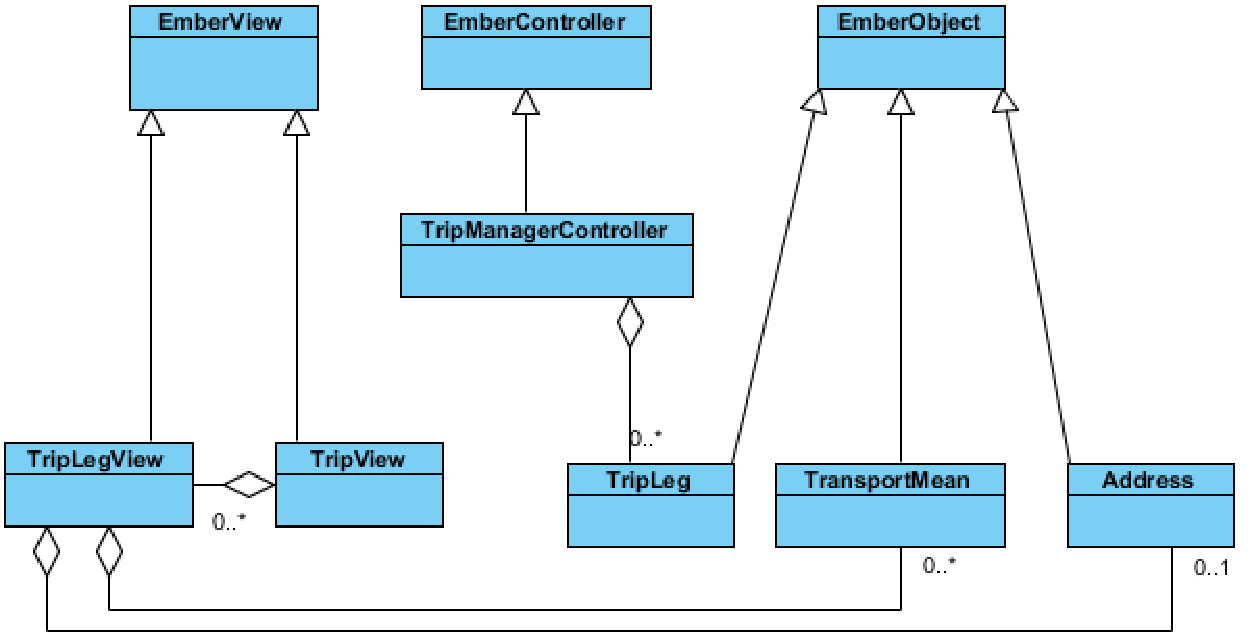
\includegraphics[scale=0.70]{./Figures/chapter4/figure7.pdf}
		\rule{35em}{0.5pt}
	\caption[Front-end class diagram comprising classes used in trip management tasks]{Front-end class diagram comprising classes used in trip management tasks}
	\label{fig:frontEndClassDiagramTripManagement}
\end{figure}

\begin{figure}[htbp]
	\centering
		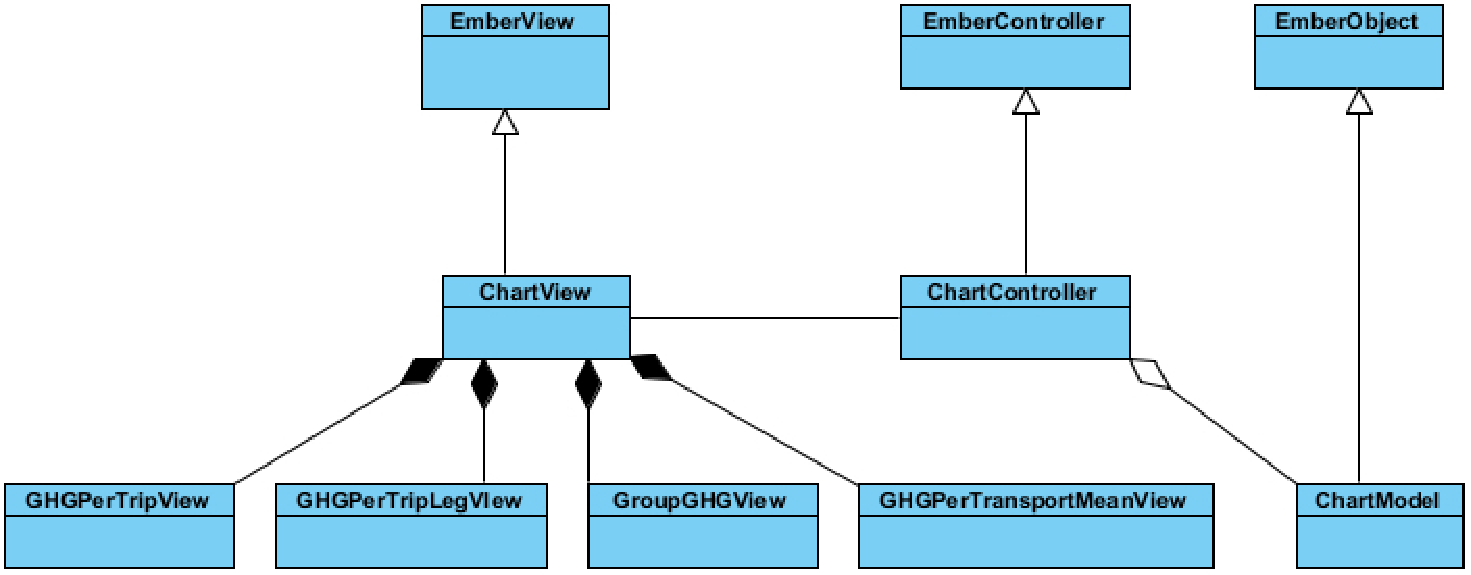
\includegraphics[scale=0.70]{./Figures/chapter4/figure8.pdf}
		\rule{35em}{0.5pt}
		\caption[Front-end class diagram comprising classes used in data visualization tasks]{Front-end class diagram comprising classes used data visualization tasks}
	\label{fig:frontEndClassDiagramVisualizationTasks}
\end{figure}

\begin{figure}[htbp]
	\centering
		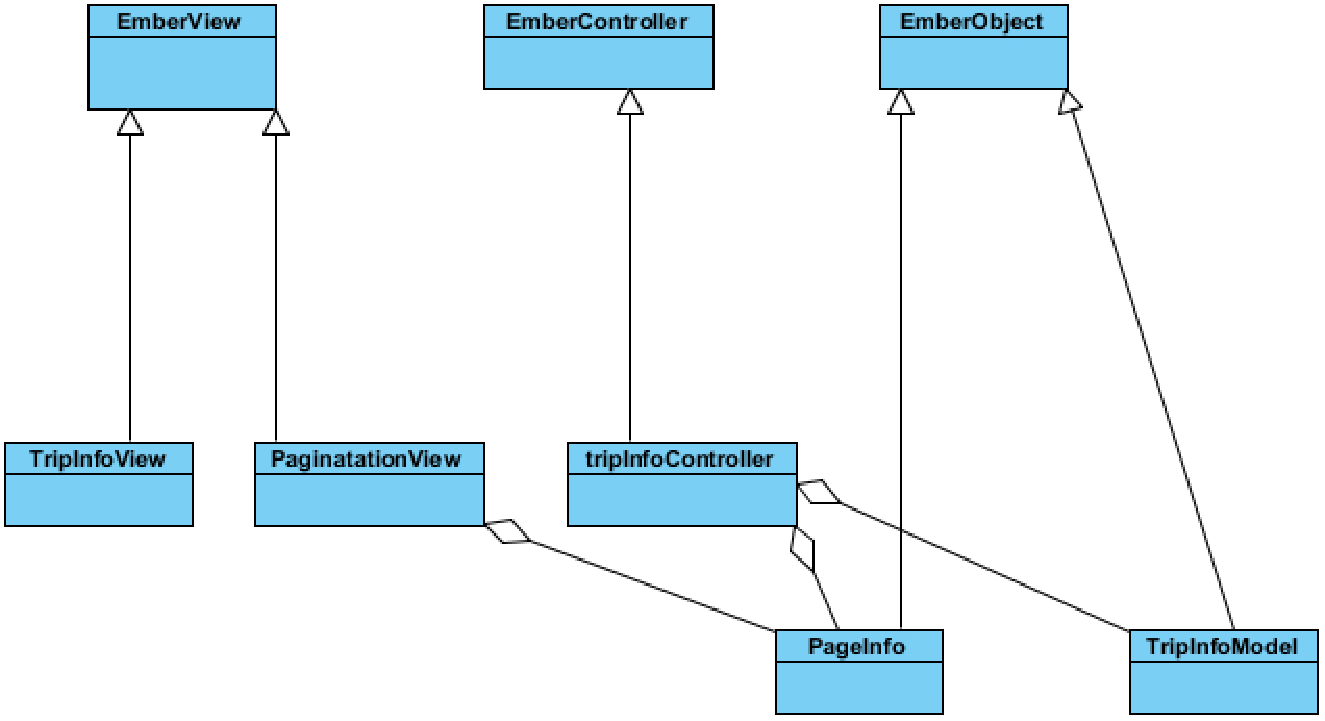
\includegraphics[scale=0.70]{./Figures/chapter4/figure11.pdf}
		\rule{35em}{0.5pt}
		\caption[Front-end class diagram comprising classes used in user trips presentation task]{Front-end class diagram comprising classes used in user trips presentation task}
	\label{fig:frontEndClassDiagramUserTripPresentationTask}
\end{figure}

\begin{table}
  \centering
  \begin{tabular}{|p{150px}|p{250px}|}
    \hline
    Class  & Description\\
    \hline
    EmberView & A class which represents views as defined by the Ember\footnote{$http://emberjs.com/$} library (Ember.View). \\
    EmberController & A class which represents controllers as defined by the Ember library (Ember.Controller). \\
    EmberObject & A class which represents models as defined by the Ember library (Ember.Object). \\
    TripManagerController & A controller responsible for gathering trip informations and sending them to the back end via AJAX Post call. \\
    TripView & A view that has an html template (i.e. html form elements) for adding information about trips. \\
    TripLegView & A view that has an html template (i.e. html form elements) for adding information about trip legs (e.g. source address, transport mena etc.). It is a sub view of the TripVew view. \\
    TripLeg & A model holding information about trip legs. \\
    TransportMean & A model that holds information about transport means. \\
    Address & A model that holds information about geographical addresse. \\
    ChartView & A view that has an html template for displaying several charts. Those charts are hosted within GHGPerTripView, GHGPerTripLegView, GroupGHGView, GHGPerTransportMeanView views. \\
    ChartModel & A model containing appropriate data that are passed as input to a JavaScript charting library. \\
    TripInfoView & A view that has an html template for displaying the trips that a used has done. \\
    PaginationView & A view containing a paginator\footnote{$http://en.wikipedia.org/wiki/Pagination$}, which helps to navigate through a list of trips. \\
    tripInfoController & A controller that fetched information about trip from the back-end via AJAX GET requests. \\
    TripInfoModel & A model containing information about trips. \\
    PageInfo & A model containing information that are required by the paginator. \\
    \hline
  \end{tabular}
  \caption{Front-end classes}\label{frontEndClasses}
\end{table}


\subsection{Database Schema}

The data model for our ampliation was probably the most important part, after capturing the requirements and forming the use cases. The application stores all data in a relational database which consists of 48 relations. More specifically, there are three sets of tables for different reasons. There is a set of tables supporting the authentication and authorization mechanism; another set used for storing provenance information; and finally a third set of tables storing the rest data produced by the application (e.g. user trips, carbon emissions, transport means etc.). Figure \ref{fig:databaseSchema} presents the database schema including tables of the third set. A brief description for each table is summarizes in table \ref{databaseTables}. Note that the database schema is missing several other tables which share similar features, such as all the other modes of transports apart from cars and their corresponding carbon emissions.

\begin{landscape}
    \begin{figure}[htbp]
	\centering
		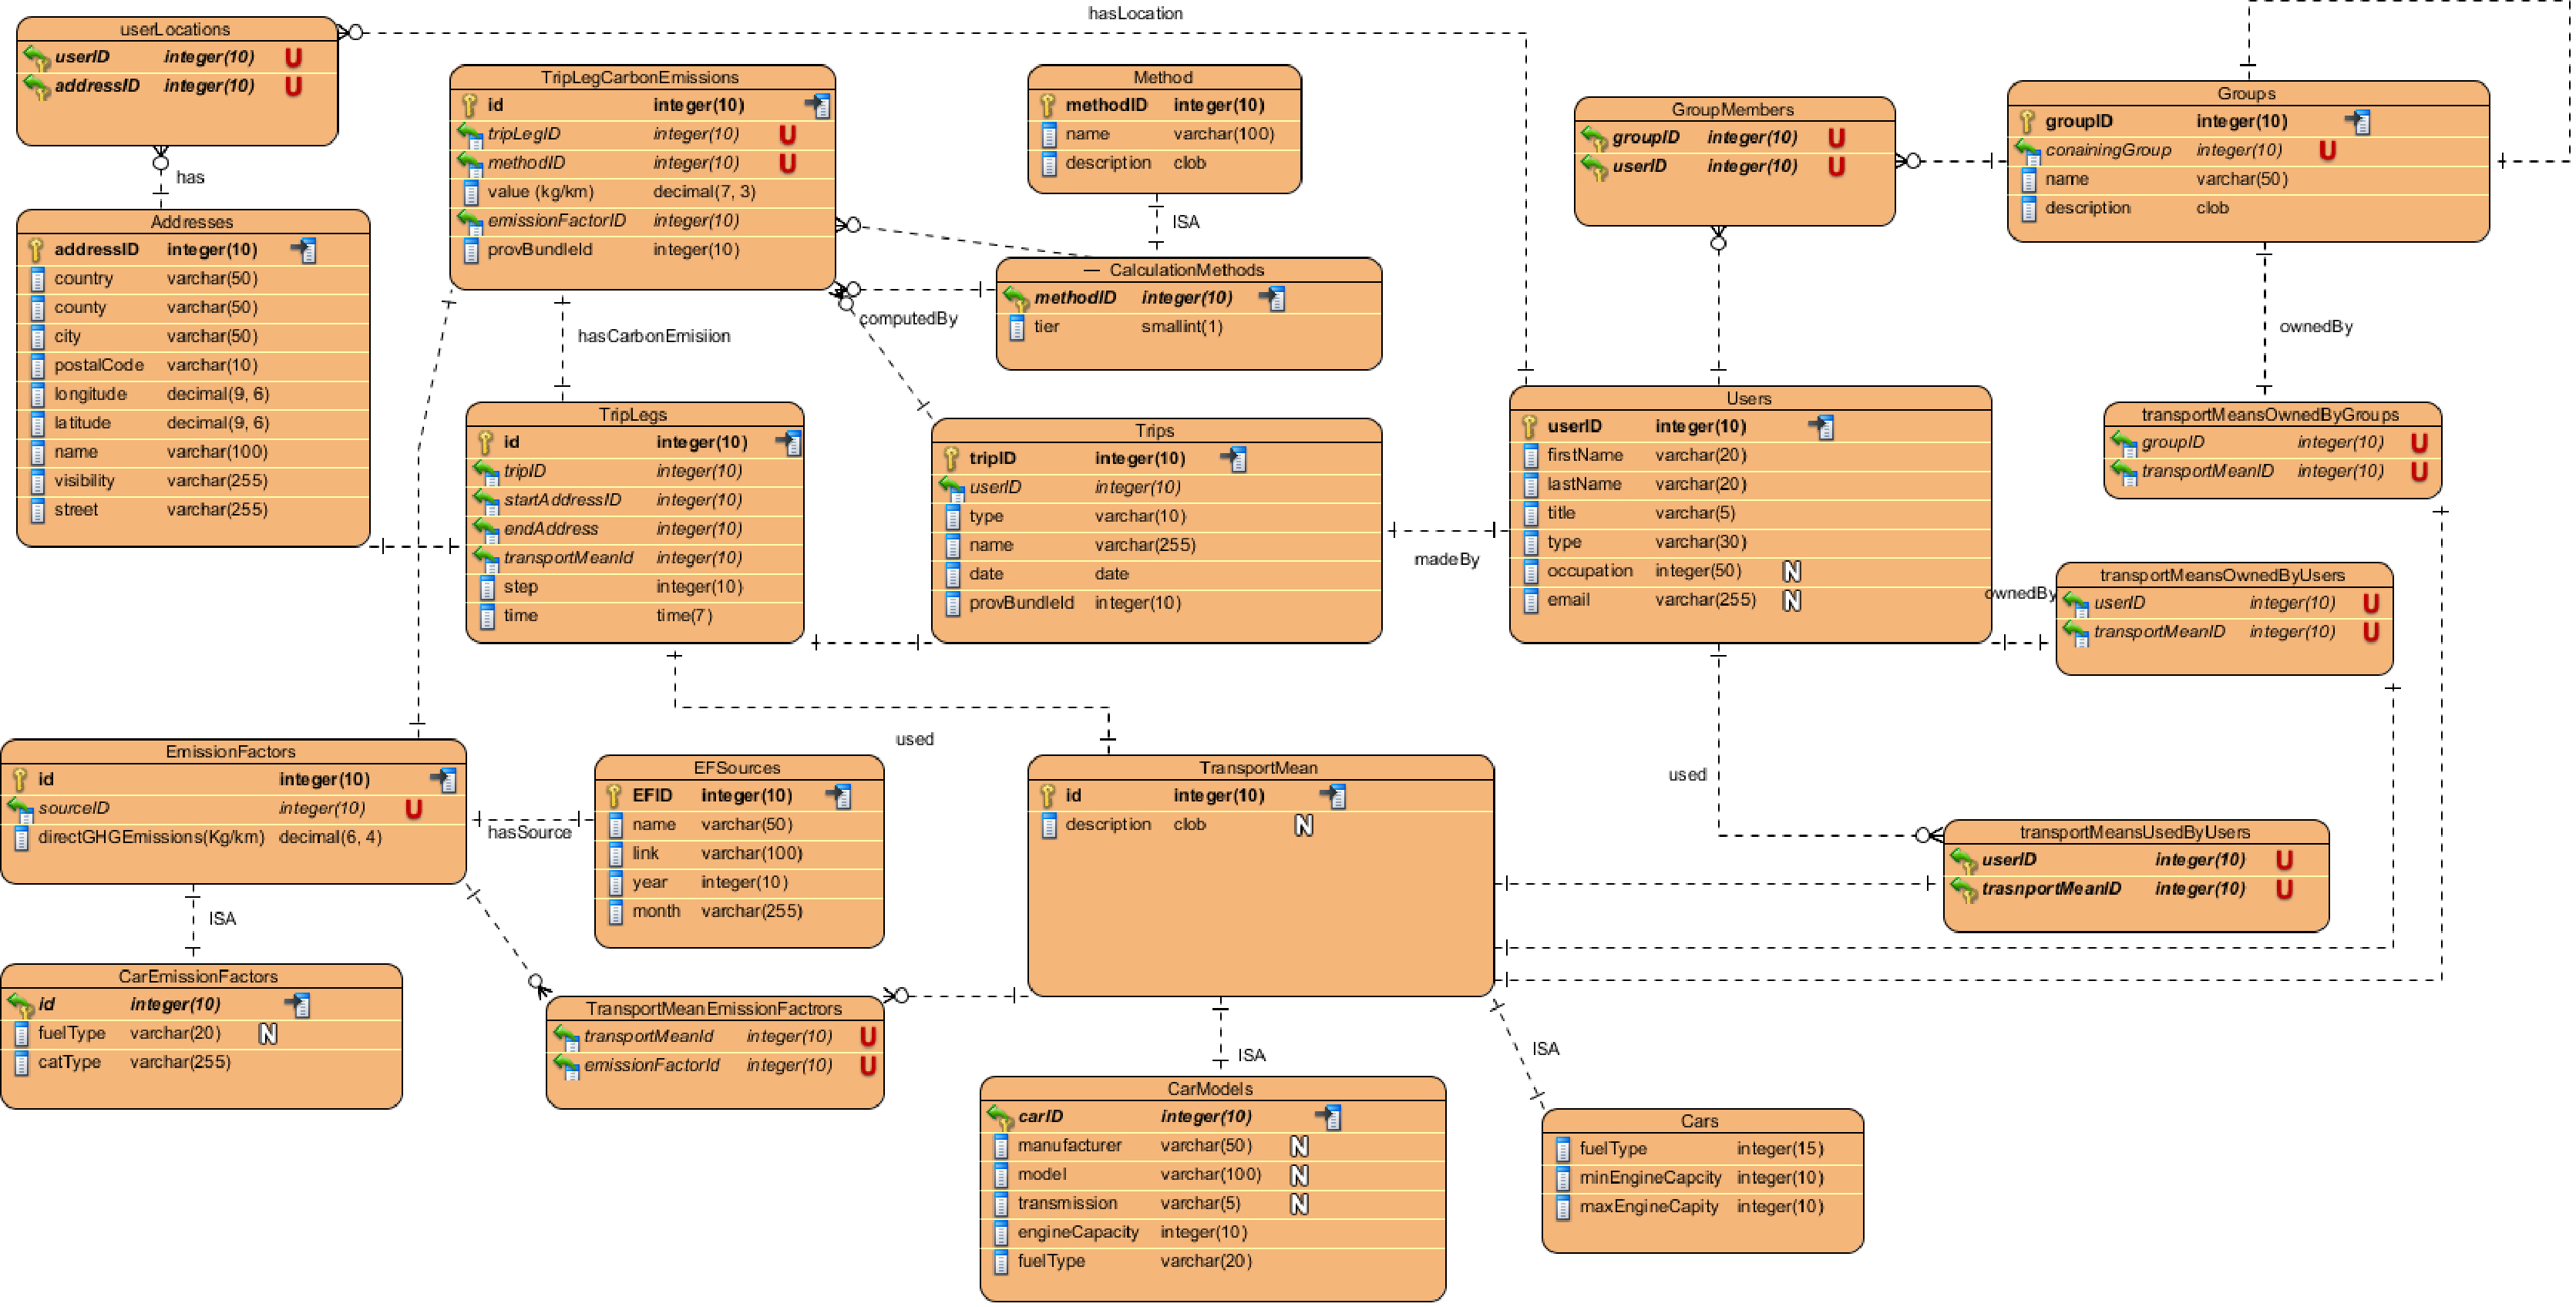
\includegraphics[scale=0.43]{./Figures/chapter4/figure9.pdf}
		\rule{35em}{0.5pt}
	\caption[Database schema]{Database schema}
	\label{fig:databaseSchema}
\end{figure}
\end{landscape}

\begin{table}
  \centering
  \begin{tabular}{|p{150px}|p{250px}|}
    \hline
    Relation  & Description\\
    \hline
    Trips & Table containing the trips made by students and the members of the university staff. \\ \hline
    TripLegs & Table storing the intermediary steps of a trip. \\ \hline
    TripLegCarbonEmissions & Table containing the calculated value of carbon emissions caused by trip legs. \\ \hline
    Method & Table containing description about different sort of methods employed by the application. For example, an extrapolation method for calculating the annual carbon emissions for an individual, based on partial set of trips that were added. \\ \hline
    CalculationMethos & Special case of the Method relation. It contains various methods for calculating carbon emissions. \\ \hline
    UserLocations & A table containing the locations that user has visited. \\ \hline
    Addresses & Table containing details about geographical addresses. \\ \hline
    TransportMean & A abstract relation that has concrete relations storing different modes of transports. CarsModels and Cars and is an example of such concrete relation. \\ \hline
    EmissionFactors &  A abstract relation that has concrete relations storing emission factors for different modes of transports. CarEmissionFactors is an example of such concrete relation \\ \hline
    TransportMeanEmissionFactors & A many-to-many relation between emission factors and transport means. Each transport mean can have different emission factors based in the source that provides them. \\ \hline
    EFSource & Table containing the sources of emission factors (e.g. IPCC etc.) \\ \hline
    Users & Table containing the users of our application. \\ \hline
    Groups & Any group that contains a number of people, such as a research group, an academic unit or the entire university. \\ \hline
    GroupMembers & Table containing the members (users) of each group. \\ \hline
    TransportMeansUsedByUsers & Table contains the transport that users have used. \\ \hline
    TransportMeansOwnedByUsers & Table contains transport means that users own. \\ \hline
    TransportMeansOwnedByGroups & Table contains transport means owned by groups. \\

    \hline

  \end{tabular}
  \caption{Database tables}\label{databaseTables}
\end{table}

\section{Summary}

In this chapter we went through the application's design phase. To make the description more obvious, various types of UML diagrams were given illustrating the path we followed towards implementing the application.

 % Experimental Setup

%% Chapter 1

\chapter{Provenance in the Application's Context} % Write in your own chapter title
\label{Provenance in the Application Context}
\lhead{Chapter 4. \emph{Provenance in the Application Context}} % Write in your own chapter title to set the page header

\section{introduction}

In the previous section we have extensively covered the concept of provenance of electronic data. We went through the benefits of capturing provenance information. We then presented different data models for representing, as well as, locating and retrieving that information. The purpose of this chapter is to describe all those concepts, in the scope of the web application that we developed. We will start by reviewing the benefits that provenance brought to our application. Then the data for which provenance is tracked, will be presented. Finally, we briefly describe how the application stores and exposes that information to external applications.

\section{Benefits of Provenance}

Our web application is a provenance-aware crowd sourced system for monitoring GHG emissions caused by commuter travels. In essence, users are the main source of information; they insert some data pertaining to the travels they make and the application calculates the GHG emissions they produce. It is critical for users to be able to verify the correctness of such calculations. To make that possible, the application needs to track all the steps in the carbon emissions calculation process: the module responsible for calculating carbon emissions has to compile all emissions sources for the subject (in the context of this application, emission sources refer to the trip made by users). Then, an appropriate method for quantifying the emissions of each source has to be selected. Finally, the data required by the method should be gathered, so that carbon emissions for the trip in question can be computed.
In order to verify and validate the computed figure, one should be able to view details for each of those steps; for instance, consider that the total amount of carbon emissions of an individual needs to be verified. In that case, the emission sources that were used have to be presented. Further, the calculation methods, as well as, the data used (i.e. activity data and emission factors), need to be examined.
It is obvious that all the aforementioned data are already stored in the applications' persistence storage (i.e. database). However, what is missing are the connections (dependencies) between those data. This gap is filled by implementing a software component responsible for provenance related tasks. What follows is a descriptions of those tasks.

\section{Tracking Provenance}

In this section we will explain how our application captures, stores and exposes provenance information. We start by presenting the provenance graphs that represent that information.

\subsection{Trip Creation Process}

One of the chief functionalities provided by the application is the insertion of trips. Users, add with the aid of an interactive web UI (refer to chapter 5 for more details) the trips that they make.
The provenance manager, which is the system's component responsible for provenance-related tasks, creates a provenance graph during the process of creating new trips (the "trip creation" process). Figure \ref{fig:provTripCreationGraph}, illustrates a visualized form of that graph, which reveals the provenance of a trip made by the user.

\begin{figure}[htbp]
	\centering
		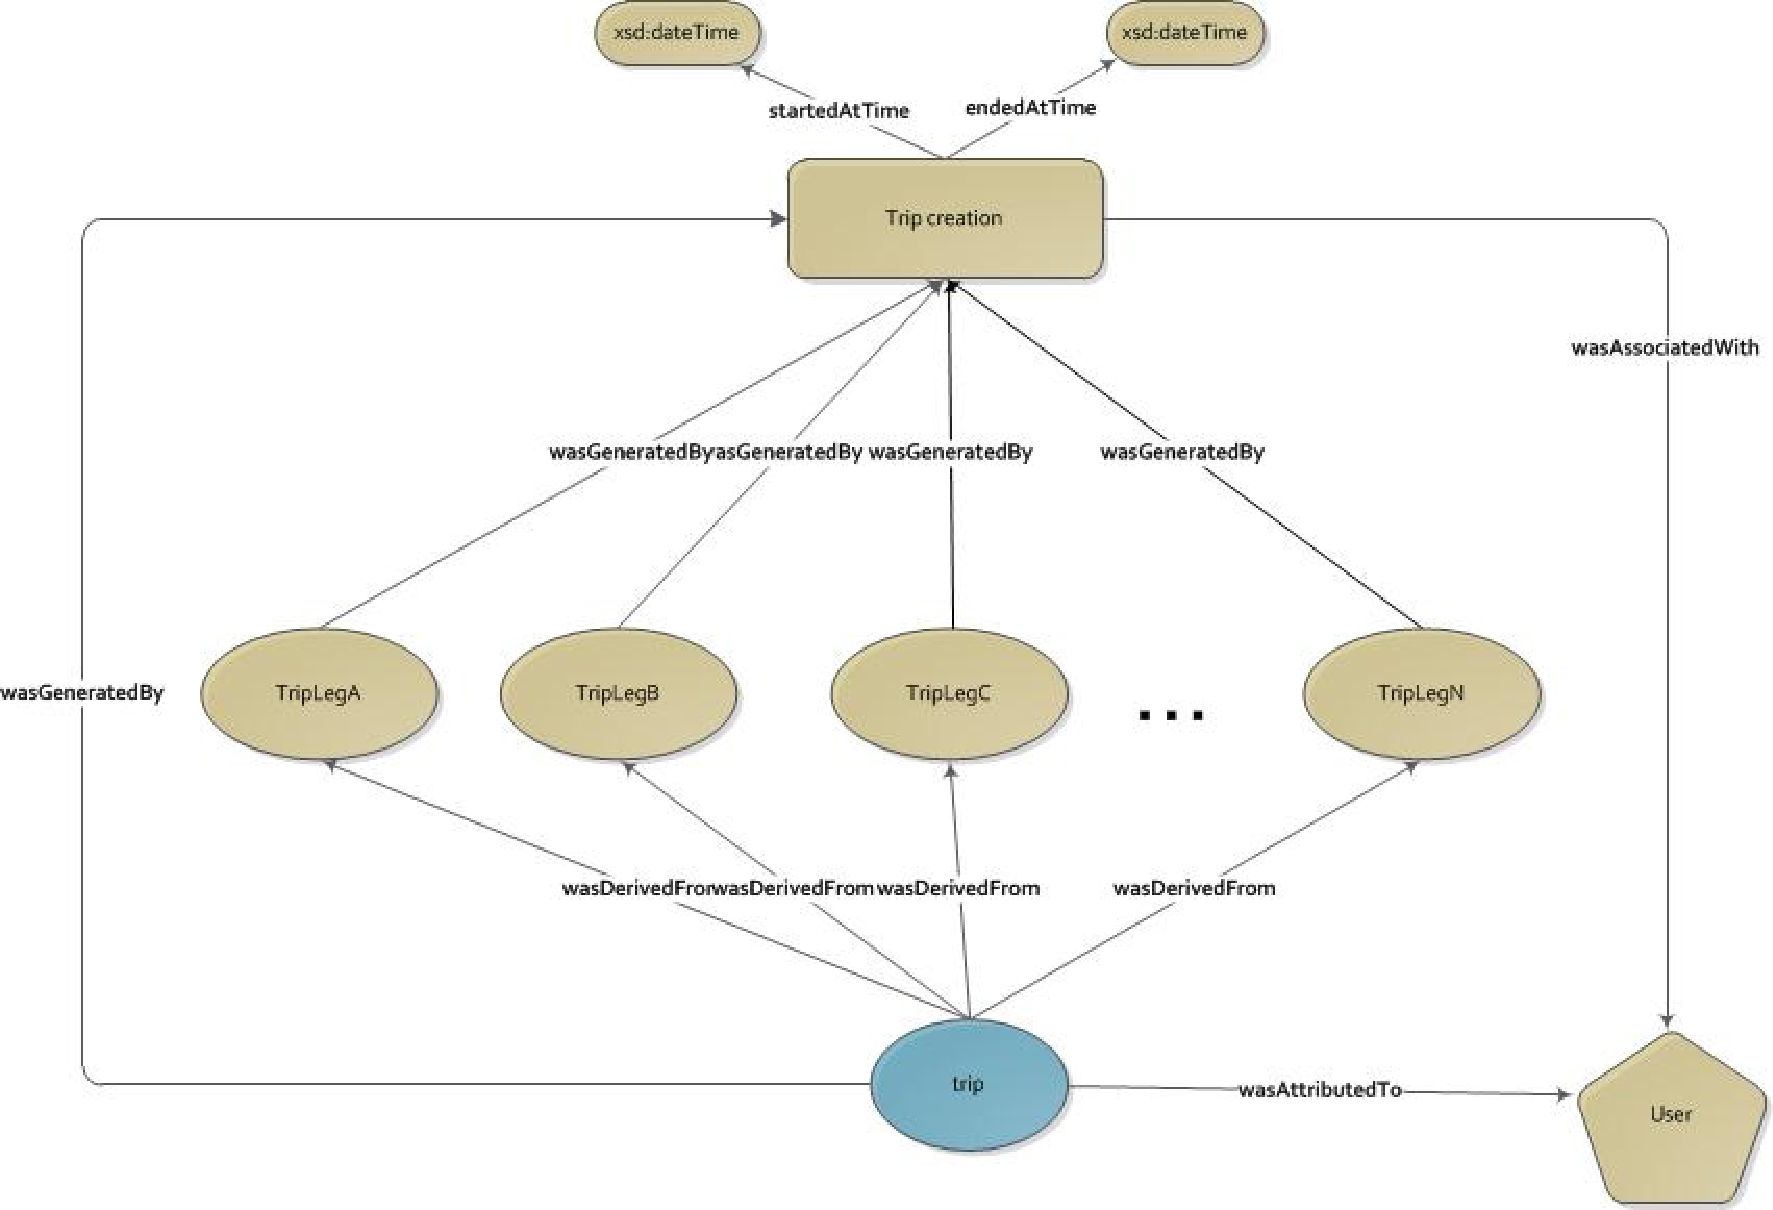
\includegraphics[scale=0.60]{./Figures/chapter3/figure1.pdf}
		\rule{35em}{0.5pt}
	\caption[Trip creation provenance graph]{Trip creation provenance graph.}
	\label{fig:provTripCreationGraph}
\end{figure}

The application adopts the PROV-DM model to represent provenance information. For this reason the graph in figure \ref{fig:provTripCreationGraph} consists of entities, activities and agents, as well as, the relationships among them.

The trip entity refers to the trip that was created during the "trip creation" process.  Each trip might consist of several intermediary steps, which we call "trip legs". This is the reason why the \emph{wasDerivedFrom} property connects the trip entity with the corresponding trip legs entities.

Each trip and trip leg is created (\emph{wasGeneratedBy} edge) via the "trip creation" process, which corresponds to the "TripCreation" activity. In some cases it is required to know the computational time of that activity. For this reason the provenance graph includes two additional nodes, storing the start and end time of that activity. Finally users are responsible for creating new trip. Hence, an agent node is added denoting that users has a degree of responsibility for the "Trip Creation" activity.

\subsection{Trip Leg Calculation Process}

During the "Trip creation" process, the system initiates the "Trip Leg Calculation" process. This process, calculates the carbon emissions for each trip leg, based on the data provided by the user. It is the responsibility of this process to select the activity data and an appropriate emission factor (based on the mode of transport used) that will be used in the calculation formula.

The provenance graph that is created during this phase is illustrated in figure \ref{fig:provTripLegCo2Graph}.

\begin{figure}[htbp]
	\centering
		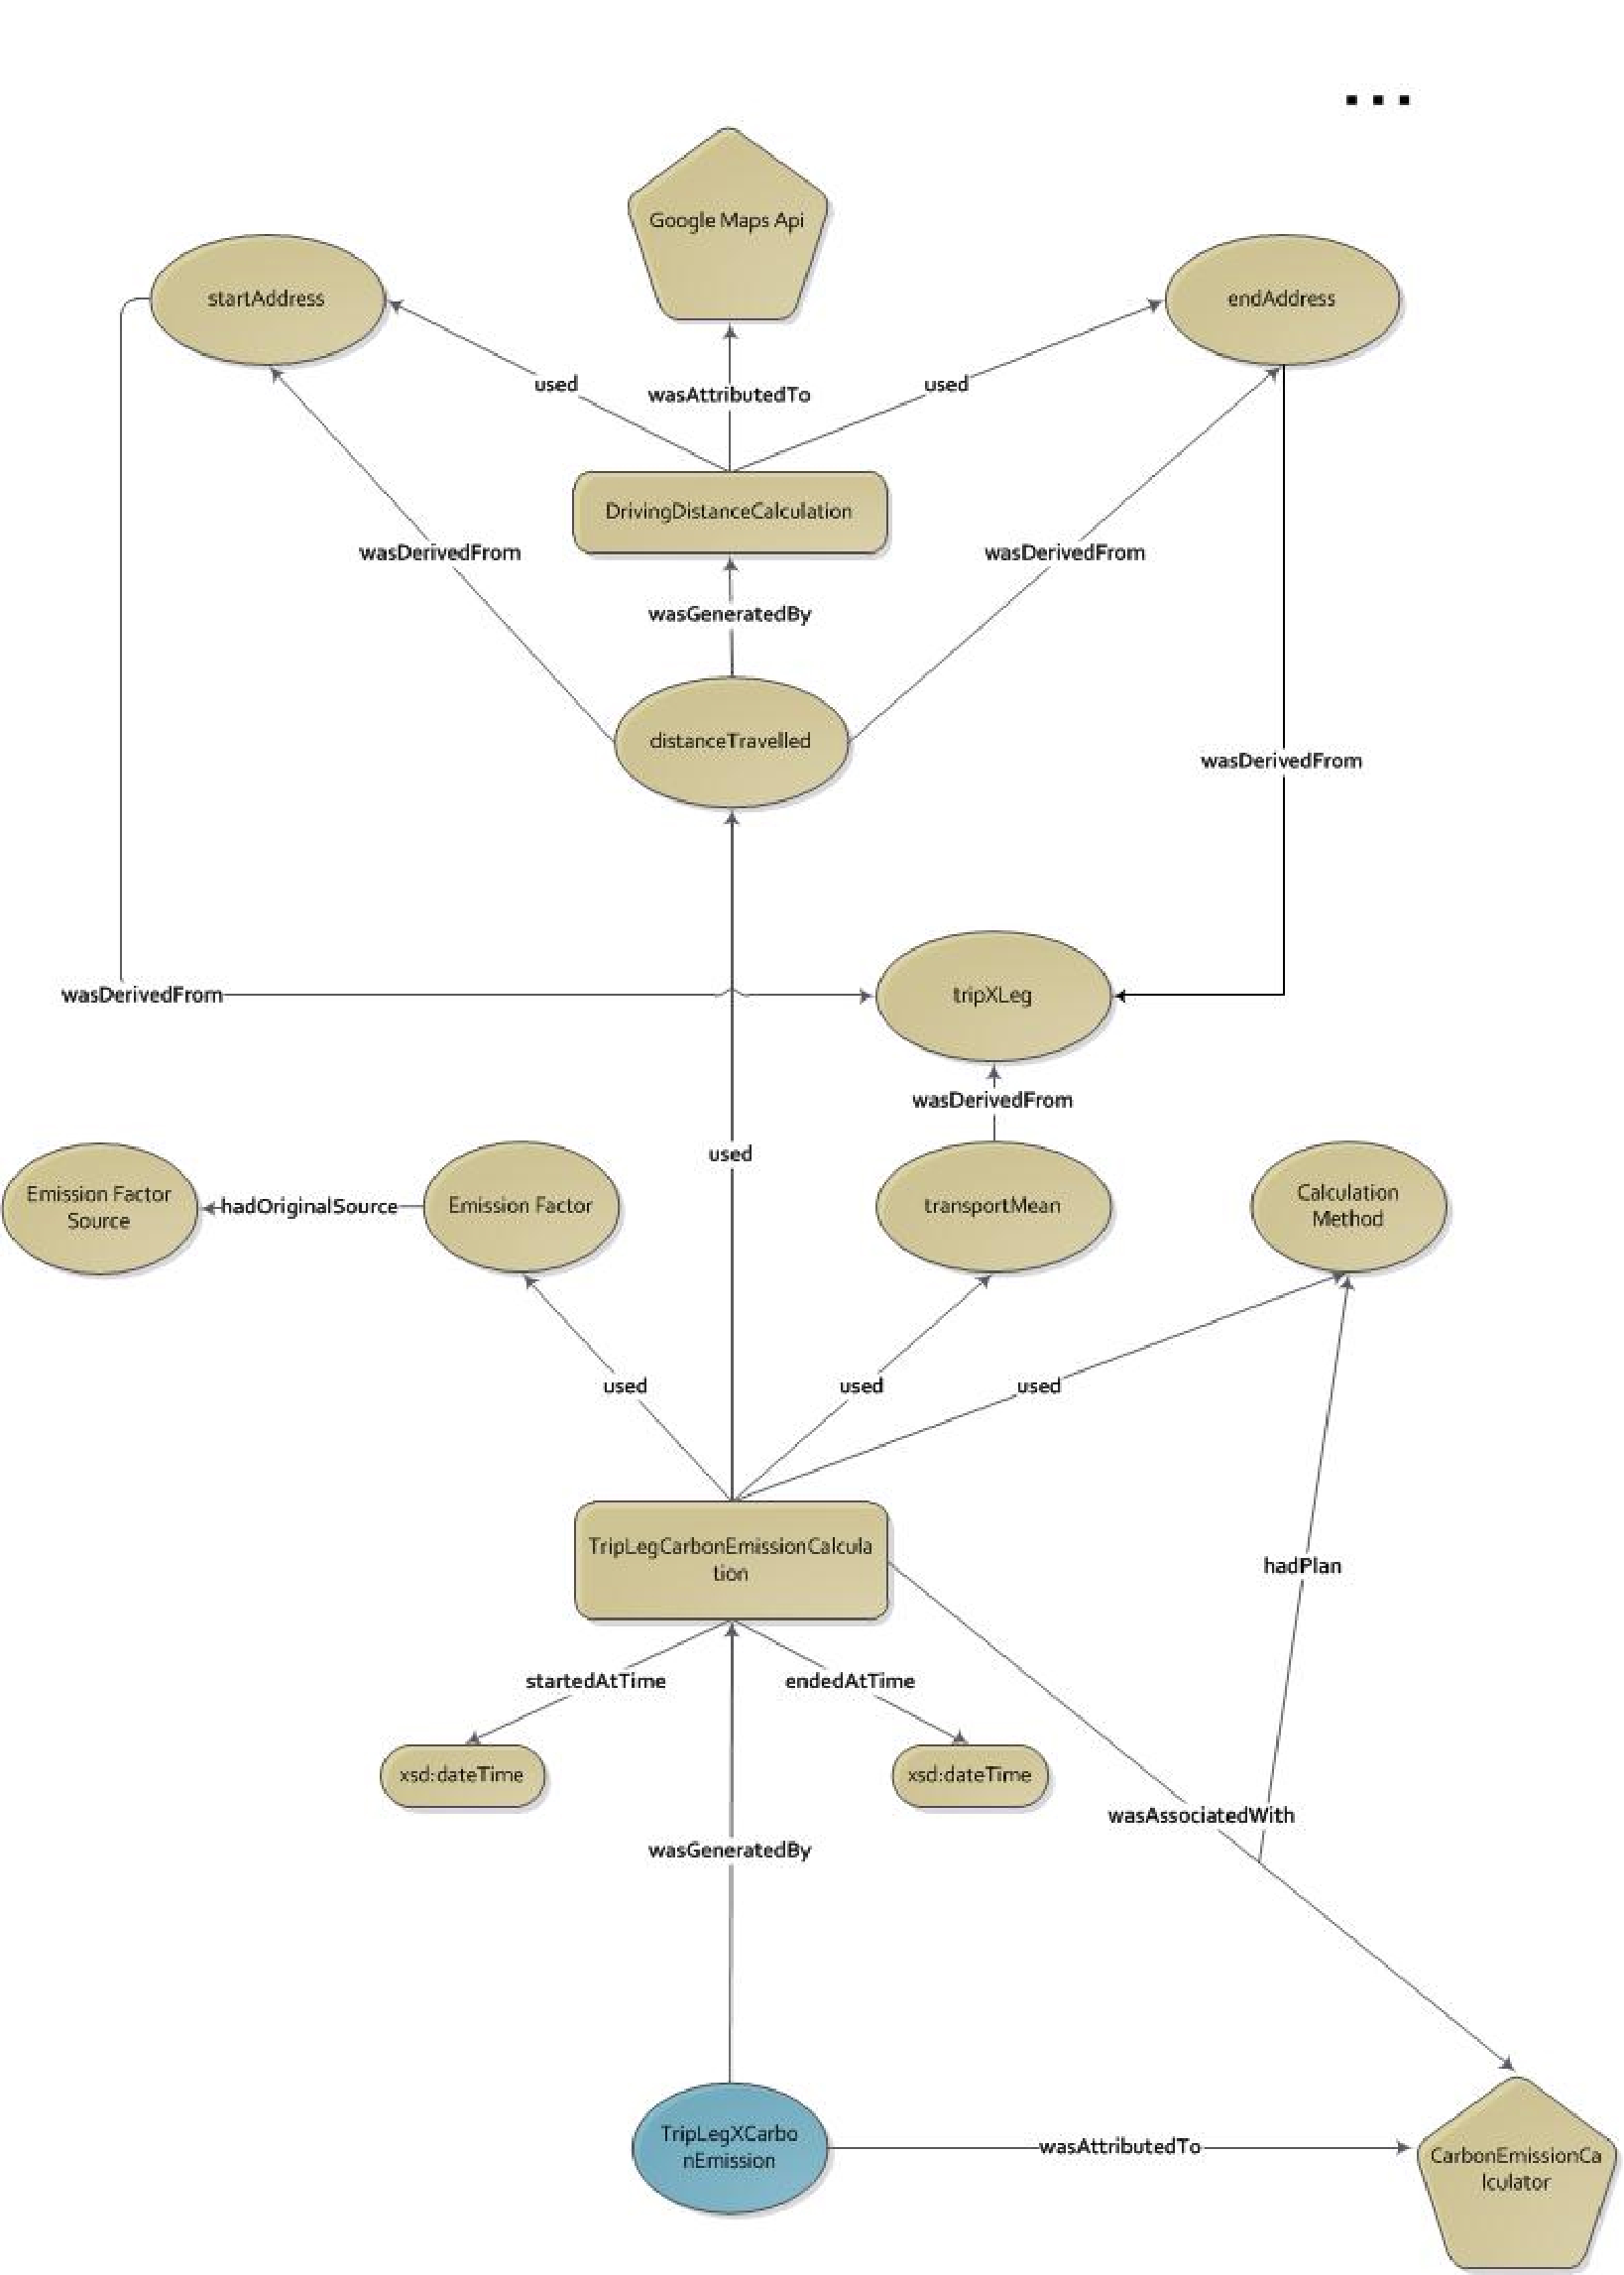
\includegraphics[scale=0.60]{./Figures/chapter3/figure2.pdf}
		\rule{35em}{0.5pt}
	\caption[Graph illustrating the provenance of the TripXLegCarbonEmission entity]{Graph illustrating the provenance of the TripXLegCarbonEmission entity.}
	\label{fig:provTripLegCo2Graph}
\end{figure}

The "TripLegCarbonEmissionsCalculation" activity, which is initiated by the "CarbonEMissionCalculation" agent, corresponds to the process of computing the carbon emissions for a specific trip leg.  The calculation process needs some sort of activity data and appropriate emissions factor, based on the mode of transport used. Ultimately, those data are combined via a calculation method to produce the carbon emissions for that trip leg. The relationship is expressed via the used edges from the "TripLegCarbonEmissionsCalculation".

The "distanceTravelled" entity represents the driving distance travelled by the transport mean. This figure is computed dynamically through a service (DrivingDistanceCalculation) provided by a third party application (GoogleMaps API). The input data for this service are the source and destination addresses of the trip. Finally, there can be several organizations that publish emission factors; we need to explicitly specify the source of the emission factor. For this reason, the \emph{hadPrimarySource} edge from "emissionsFactor" to "emissionFactor Source" is added.


\subsection{Trip Carbon Emissions Calculation Process}

The process of calculating the total carbon emissions caused by a trip is relatively straightforward. It simply sums together the carbon emissions caused by all the intermediary trip legs.

\begin{figure}[htbp]
	\centering
		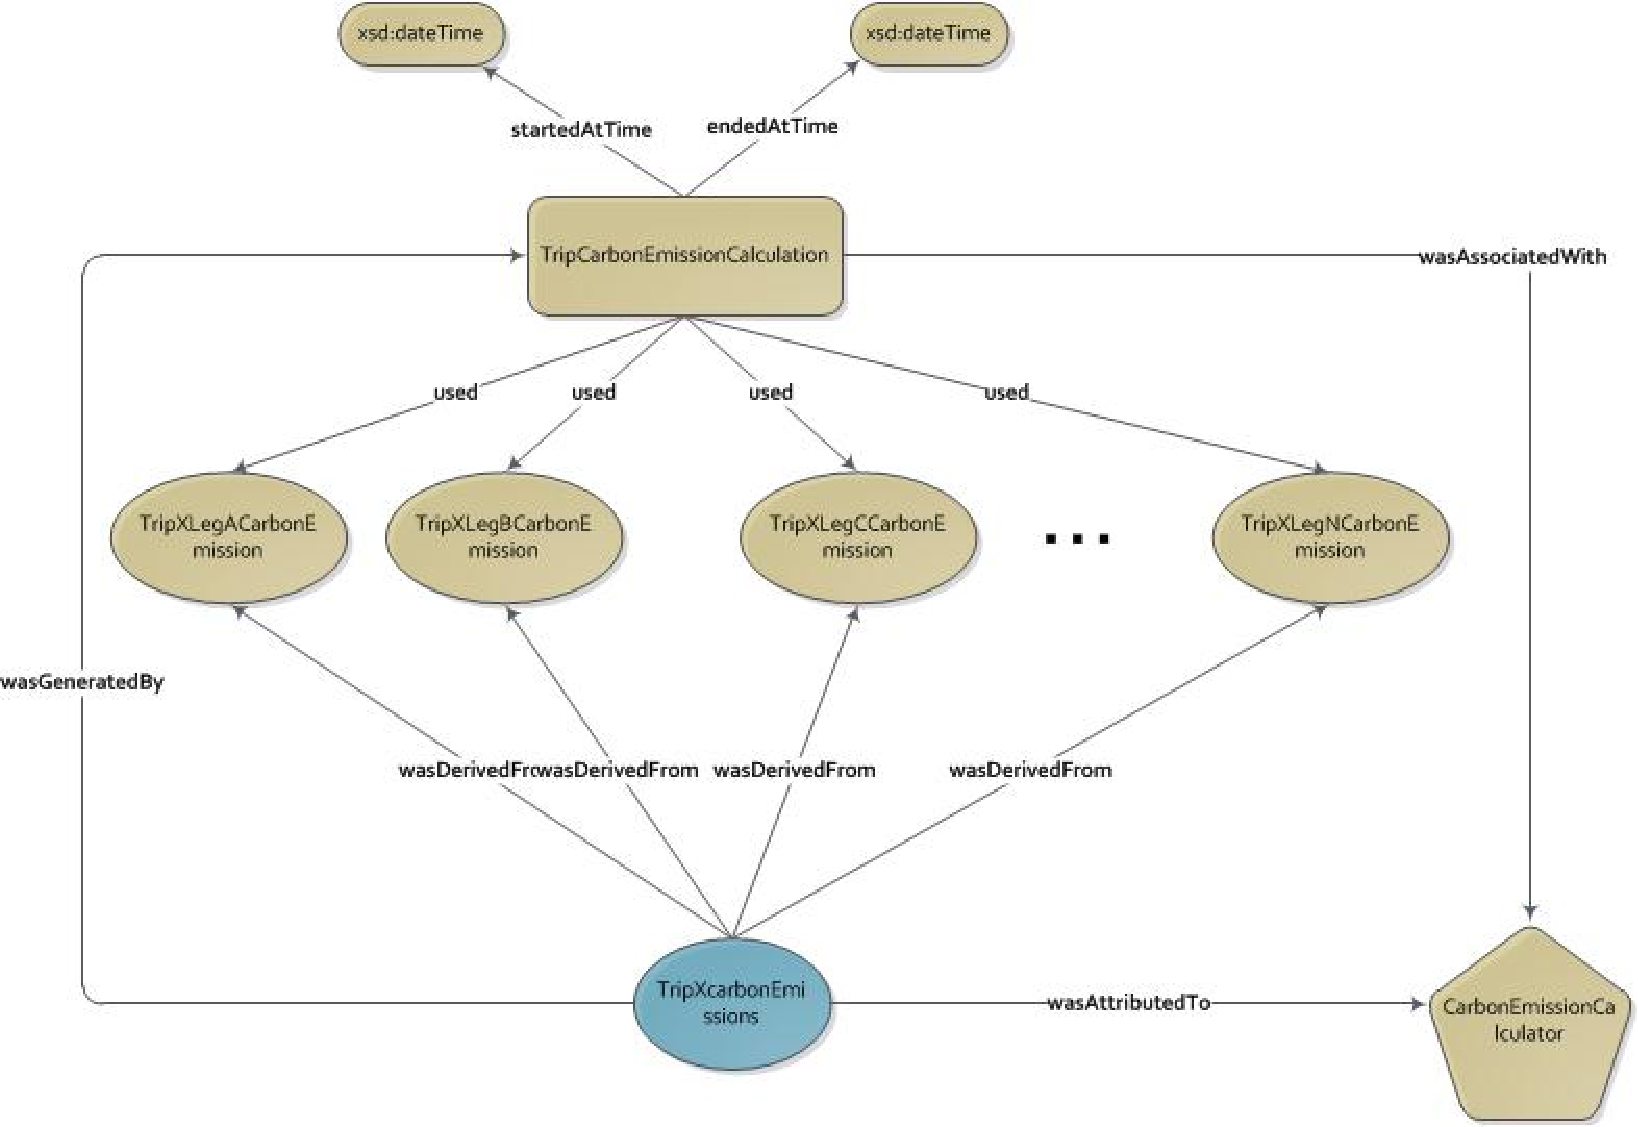
\includegraphics[scale=0.60]{./Figures/chapter3/figure3.pdf}
		\rule{35em}{0.5pt}
	\caption[ Graph illustrating the provenance of the carbon emissions of a trip]{ Graph illustrating the provenance of the carbon emissions of a trip}
	\label{fig:provTripCo2Graph}
\end{figure}

Figure \ref{fig:provTripCo2Graph} demonstrates a graph that describes the provenance the carbon emissions caused by a trip, that is, how that value was derived. The calculation of carbon emissions is processed by the "TripCarbonEmissionCalculation" activity, which sums the the carbon emissions of all the intermediary trip legs to compute that total emissions for the trip (TripXCarbonEMissions).  The dependency is represented via \emph{wasDerivedFrom} edges. Finally, the "CarbonEmisisonCalculator" agent is responsible for undertaking the whole process.

This is good point to demonstrate an example describing how a provenance graph can help users validate their carbon emissions. Consider a scenario where the user modifies the data for one trip leg of a hypothetical trip (TripX). Assume that she changed the transport mean used during that trip leg. At some point, though, she realizes that there is a significant fluctuation between the old and the new value. More specifically, the new carbon emissions value for TripX is much higher than the previous one. In order to verify that there was no error during the calculation process; user can navigate through the provenance of that value (see figure \ref{fig:provTripCo2GraphRevision}).


\begin{figure}[htbp]
	\centering
		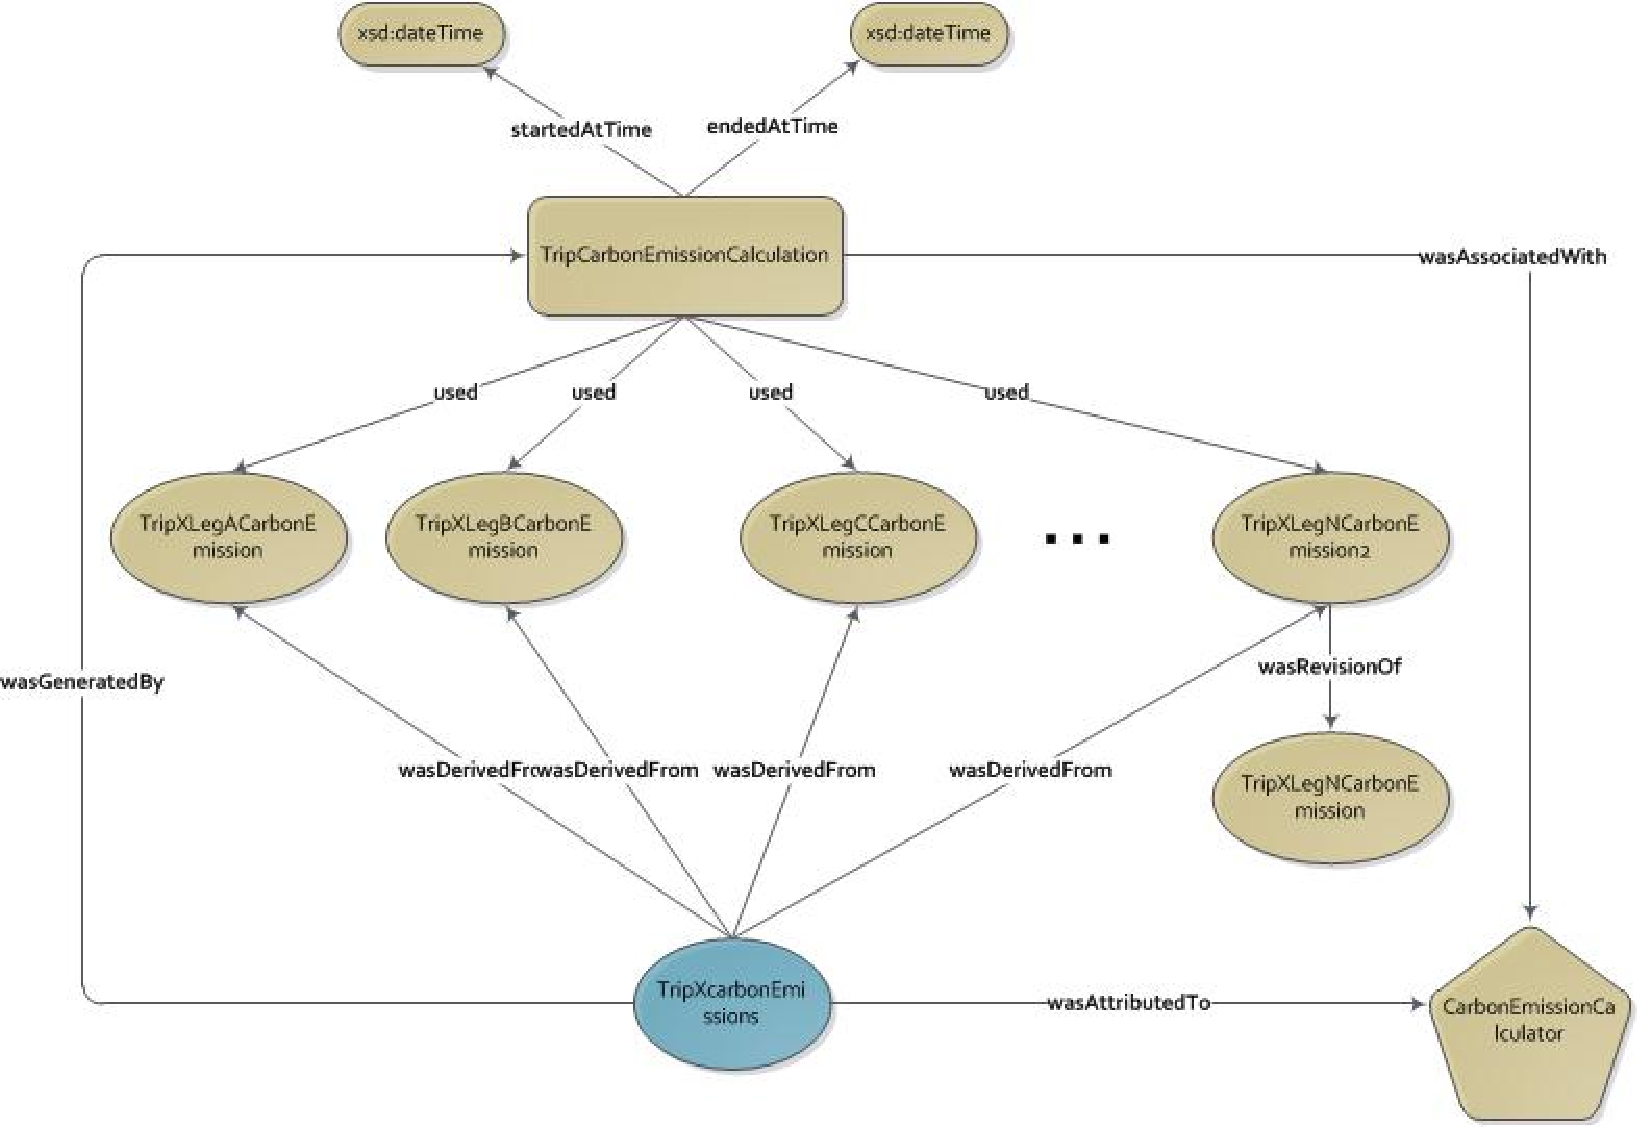
\includegraphics[scale=0.60]{./Figures/chapter3/figure4.pdf}
		\rule{35em}{0.5pt}
	\caption[Graph illustrating the provenance of the carbon emissions of a trip after a trip leg was modified]{Graph illustrating the provenance of the carbon emissions of a trip after a trip leg was modified}
	\label{fig:provTripCo2GraphRevision}
\end{figure}

The graph reveals that the "TripXLegNCarbonEmission" entity has been modified and replaced by the "TripXLegNCarbonEmission2" entity. Ultimately, by investigating the provenance of the new entity (the provenance graph is similar to the one illustrated in figure \ref{fig:provTripLegCo2Graph}), she realizes that she has accidentally inserted the wrong transport mean.

The same approach can be followed when the validation for values for which provenance information is stored, is needed.


\subsection{Calculation process for individual and group carbon emissions}

The application gives a chance for users to view a report where details about individual carbon emissions are presented. One of the information included in that report is the total carbon emissions caused by all the trips made by the user. To achieve that, the carbon emissions for all trips are summed together.

\begin{figure}[htbp]
	\centering
		\includegraphics[scale=0.60]{./Figures/chapter3/figure5.pdf}
		\rule{35em}{0.5pt}
	\caption[Graph illustrating the provenance for individual carbon emissions]{Graph illustrating the provenance for individual carbon emissions}
	\label{fig:provIndividualCo2Graph}
\end{figure}

The same approach is adopted by the "Group Calculation" process, whereby the carbon emissions caused by all the trips made by all the members of the group in question are summed together. Figure \ref{fig:provGroupCo2Graph} illustrates the provenance graph for group carbon emissions.

\begin{figure}[htbp]
	\centering
		\includegraphics[scale=0.60]{./Figures/chapter3/figure6.pdf}
		\rule{35em}{0.5pt}
	\caption[Graph illustrating the provenance for group carbon emissions]{Graph illustrating the provenance for group carbon emissions}
	\label{fig:provGroupCo2Graph}
\end{figure}

\section{Storing Provenance}

The provenance graphs that we discussed earlier are represented in some application-specific format and stored in a relational database. More details about the process of creating and storing provenance graphs are presented in the next chapter.

\section{Fetching Provenance Information}

Our application has two options for viewing the provenance information for a specific piece of data; for instance, if users what to view provenance information in the form of graphs (like the above graphs), then a specific user interface can be used (next chapter describes this interface). Additionally, the application provides a REST web service that gets the identifier of a provenance graph and returns the graph in JSON format.

The JSON data below was returned after accessing the following service: http://127.0.0.1:8000/get-prov-graph/?provBundleId=1


\begin{verbatim}
{
   "wasDerivedFrom":{
      "_:id4":{
         "prov:usedEntity":"cf:tripLeg-2",
         "prov:generatedEntity":"cf:trip-1"
      },
      "_:id2":{
         "prov:usedEntity":"cf:tripLeg-1",
         "prov:generatedEntity":"cf:trip-1"
      }
   },
   "wasAssociatedWith":{
      "_:id6":{
         "prov:agent":"cf:ppoliani",
         "prov:activity":"cf:tripCreation"
      }
   },
   "wasAttributedTo":{
      "_:id7":{
         "prov:entity":"cf:trip-1",
         "prov:agent":"cf:ppoliani"
      }
   },
   "agent":{
      "cf:ppoliani":{
         "prov:type":"prov:Person",
         "foaf:mbox":"<mailto:ppoliani@gmail.com>"
      }
   },
   "entity":{
      "cf:tripLeg-1":{

      },
      "cf:trip-1":{

      },
      "cf:tripLeg-2":{

      }
   },
   "prefix":{
      "foaf":"http://xmlns.com/foaf/0.1/",
      "cf":"http://users.ecs.soton.ac.uk/pp6g11/ontology/carbonFooprints/"
   },
   "activity":{
      "cf:tripCreation":{

      }
   },
   "wasGeneratedBy":{
      "_:id5":{
         "prov:entity":"cf:trip-1",
         "prov:activity":"cf:tripCreation"
      },
      "_:id1":{
         "prov:entity":"cf:tripLeg-1",
         "prov:activity":"cf:tripCreation"
      },
      "_:id3":{
         "prov:entity":"cf:tripLeg-2",
         "prov:activity":"cf:tripCreation"
      }
   }
}

\end{verbatim}

Apparently, the above representation of provenance graphs is not for human consumption. It can rather be processed by a tool that is capable of reading and understanding this sort of serializations.

\section{Summary}

In this chapter we have described the benefits of adapting the provenance of electronic data technology in our application. We presented the processes during which the provenance information is captured and illustrated that information in the form of graphs. Finally, a very brief description about the storage and exposure of the captured provenance information was presented. We will come back to those issues in the following chapter.  % Experiment 1

%% Chapter 1

\chapter{Application Implementation} % Write in your own chapter title
\label{Application Implementationn}
\lhead{Chapter 5. \emph{Application Implementation}} % Write in your own chapter title to set the page header

\section{introduction}

In chapter 3 we summarized the sequence of actions that occurred during the application's design part. In this chapter we will go through the implementation phase, outlining the core functionalities of the application. In addition, screen shots illustrating the application in action will be provided. Furthermore, a description about how the application was tested will be presented, along with the appropriate unit tests that were run. The chapter ends with a discussion and criticism about the final outcome of the implementation phase along with future work.

\section{Application's Implementation Phase}

In this section we will present how the application was implemented based on the decisions that were taken during the design phase. More specifically, we will introduce a set of sequence diagrams, illustrating the flow of function calls. The diagrams will be accompanied by a brief description, as well as, several screenshots showing the application in action.

\subsection{Add Trip}

As explained earlier, this use case requires users to insert the trips that they make during the course of time. The sequence diagram in figure \ref{fig:addTripInfoSeqDiagram} illustrates the process of adding information about the trips, whereas the sequence diagram in figure \ref{fig:tripStoreSeqDiagram} demonstrates the flow of function calls that take place so that the information users insert is stored in a persistent database.

Figure \ref{fig:addTripForm} illustrates a web user interface for the trip creation process. The red rectangle indicates the \emph{addTripview} Ember view which is the main form for adding new trips. The tripLegContainer is shadowed with the blue rectangle and is, essentially, an Ember container view\footnote{$http://docs.emberjs.com/doc=Ember.ContainerView$} capable of dynamically adding new sub-views, such as \emph{tripLegView} for each trip. Finally, the yellow rectangle shows the carView view.

The sequence diagram \ref{fig:addTripInfoSeqDiagram} shows a scenario where the user initially inserts information concerning the trip's name, type, date and number of trip legs. When choosing the number of trip legs, the \emph{tripLegContainer} is created which in turn creates a number of \emph{tripLegView} views based on the number of trip legs. Then user again needs to indicate some information about the trip leg's source and destination address, and the transport mean that was used. Selecting a transport mean, results in the creation of the \emph{tripLegTransportContainer} view, which is a dynamic view that we have used to support rich interactivity. In this scenario, user has chosen a car; therefore a \emph{carView} view (yellow rectangle) is added to the \emph{tripLegTransportContainer}. The form element in that view are populated with data that are fetched from the back-end via AJAX GET calls. Finally, after filling all the required fields, the user submits the form.

\begin{landscape}
\begin{figure}[htbp]
	\centering
		\includegraphics[scale=0.55]{./Figures/chapter4/figure10.pdf}
		\rule{35em}{0.5pt}
	\caption[Add trip information sequence diagram]{Add trip information sequence diagram}
	\label{fig:addTripInfoSeqDiagram}
\end{figure}
\end{landscape}

\begin{figure}[htbp]
	\centering
		\includegraphics[scale=0.40]{./Figures/chapter4/figure12.pdf}
		\rule{35em}{0.5pt}
	\caption[Add trip from]{Add trip form}
	\label{fig:addTripForm}
\end{figure}

The process of storing a trip starts after the user submits the trip creation form, that we described earlier. Initially, the \emph{tripManagerController} compiles the data inserted by the user and fills the corresponding models, namely tripLegModel and generalCarModel. It then makes an AJAX Post call to the back end, sending information about the trip. On the back-end, the corresponding view creates a trip model and stores it in the database. On the next step, the controller makes consequent AJAX Post request, asking for the back end to store each trip leg into the database. Finally, two more AJAX calls occur; the first asks the back-end to create a provenance graph for each trip leg, whereas the second asks for the carbon emissions of each trip leg to be calculated.

\begin{landscape}
\begin{figure}[htbp]
	\centering
		\includegraphics[scale=0.55]{./Figures/chapter4/figure13.pdf}
		\rule{35em}{0.5pt}
	\caption[Trip storing sequence diagram]{Trip storing sequence diagram}
	\label{fig:tripStoreSeqDiagram}
\end{figure}
\end{landscape}

\subsection{Show User's Trips}

The user have the chance to manage the trip that he has added to the system. More specifically, the actions that are offered are: view, edit and delete tips. Figure \ref{fig:userTrips} illustrates the web user interface that displays all user's trips. Notice that trips are categorized according to the transport means that were used.

\begin{figure}[htbp]
	\centering
		\includegraphics[scale=0.40]{./Figures/chapter4/figure14.pdf}
		\rule{35em}{0.5pt}
	\caption[UI showing user's trips]{UI showing user's trips}
	\label{fig:userTrips}
\end{figure}

As shown in the sequence diagram \ref{fig:userTripsSeqDiagram} the process is fairly simple. The \emph{tripInfoController} fetches the trips made by a car from the back-end via an AJAX GET request. The back-end, in order, retrieves those data from the database and returns the in JSON format.

\begin{landscape}
\begin{figure}[htbp]
	\centering
		\includegraphics[scale=0.55]{./Figures/chapter4/figure15.pdf}
		\rule{35em}{0.5pt}
	\caption[Displaying user's trips sequence diagram]{Displaying user's trips sequence diagram}
	\label{fig:userTripsSeqDiagram}
\end{figure}
\end{landscape}

\subsection{Carbon Footprint Report}

The prime incentive for users adding the trips they make is to present a report describing their individual, as well as, group carbon footprints. In its current state, the application supports visualization of carbon emissions in the form of line and bar charts. Furthermore, the provenance for trip legs' carbon emissions are illustrated with two types of graphs; dynamic and static provenance graphs. We will expand on that in a bit. Figure \ref{fig:reportOverview} illustrates the a small part of report html page (/report).

\begin{figure}[htbp]
	\centering
		\includegraphics[scale=0.40]{./Figures/chapter4/figure16.pdf}
		\rule{35em}{0.5pt}
	\caption[Carbon footprint report page]{Carbon footprint report page}
	\label{fig:reportOverview}
\end{figure}


\subsubsection{Individual Carbon Emissions}

Users can view a small summary of their carbon footprints at the top of the report page. In its current state, the application presents the following statistics (view figure \ref{fig:ghgPerTripLeg}).

\begin{itemize}
  \item The number of trips that a user has made overall.
  \item The total weight of greenhouse gas emissions (ghg) caused by user's travels.
  \item The minimum value of greenhouse gas emissions.
  \item The maximum value of greenhouse gas emissions.
  \item The average weight of greenhouse gas emissions (ghg) caused by user's travels.
\end{itemize}

Apart from that, the report includes four charts presenting different information each. The first chart (figure \ref{fig:ghgPerTripLeg}) summarizes the carbon emissions caused by trip legs, during a specified period of time. By default, the application shows the emissions during the current month. Nevertheless, users can define the time period with the aid of two calendar widgets that reside on the top of each chart. Additionally, all the charts can be printed and downloaded in several formats, namely in PNG, PDF, JPEG and SVG.

\begin{figure}[htbp]
	\centering
		\includegraphics[scale=0.60]{./Figures/chapter4/figure17.pdf}
		\rule{35em}{0.5pt}
	\caption[Greenhouse gas emissions per trip leg]{Greenhouse gas emissions per trip leg}
	\label{fig:ghgPerTripLeg}
\end{figure}

As a complement to that chart, users can view the provenance graph of each trip leg carbon emission value. This is done by clicking on any bar; for instance, clicking on the first bar, the provenance information describing the derivation of that value, will appear (view figure \ref{fig:provGraph}). This is a interactive graph, in that, users can relocate the nodes, zoom in and zoom out, and click on each node to view a brief description.

\begin{figure}[htbp]
	\centering
		\includegraphics[scale=0.40]{./Figures/chapter4/figure18.pdf}
		\rule{35em}{0.5pt}
	\caption[Interactive provenance graph]{Interactive provenance graph}
	\label{fig:provGraph}
\end{figure}

It is obvious that the interactivity comes at the cost of a non-intuitive visualization. That is to say, the graph is not very readable, unless user relocate manually all the nodes. As a result, a second static graph is provided (figure \ref{fig:provStaticGraph}).

\begin{figure}[htbp]
	\centering
		\includegraphics[scale=0.50]{./Figures/chapter4/figure19.pdf}
		\rule{35em}{0.5pt}
	\caption[Static provenance graph]{Static provenance graph}
	\label{fig:provStaticGraph}
\end{figure}

Greenhouse gas emissions can be summarized at the level of trips, as well. \emph{The GHG Emissions Per trip} line chart (figure \ref{fig:ghgPerTrip}), visualizes the weight of ghg emissions for each trip user made, during a specified period of time.

\begin{figure}[htbp]
	\centering
		\includegraphics[scale=0.60]{./Figures/chapter4/figure20.pdf}
		\rule{35em}{0.5pt}
	\caption[Greenhouse gas emissions per trip leg]{Greenhouse gas emissions per trip leg}
	\label{fig:ghgPerTrip}
\end{figure}

The last chart (figure \ref{fig:ghgPerTransportMean}) pertaining to individual carbon footprints, illustrates the weight of carbon emissions caused by the different modes of transports, which were used during the trips made within a specified period of time.


\begin{figure}[htbp]
	\centering
		\includegraphics[scale=0.60]{./Figures/chapter4/figure21.pdf}
		\rule{35em}{0.5pt}
	\caption[Greenhouse gas emissions per transport mean]{Greenhouse gas emissions per transport mean}
	\label{fig:ghgPerTransportMean}
\end{figure}

\subsubsection{Group Carbon Emissions}

It was a initial requirement that users can be members of different groups and that carbon emissions of those groups are trackable. Consequently, aside from individual carbon footprint report, the application presents a report for users' groups. The information is similar to that enclosed in the individual report.

\begin{itemize}
  \item The number of trips that were made by the members of all user's groups.
  \item The total weight of greenhouse gas emissions (ghg) caused by all trips made by the members of all user's groups
  \item The minimum value of greenhouse gas emissions.
  \item The maximum value of greenhouse gas emissions.
  \item The average weight of greenhouse gas emissions (ghg) caused by all trips made by the members of all user's groups
\end{itemize}

\begin{figure}[htbp]
	\centering
		\includegraphics[scale=0.60]{./Figures/chapter4/figure22.pdf}
		\rule{35em}{0.5pt}
	\caption[Group greenhouse gas emissions]{Group greenhouse gas emissions}
	\label{fig:groupGhgEmissions}
\end{figure}


\section{Evaluation via Testing}

An initial requirement after finishing implementing the application was to get users try it and express their experience. However, this requirement changed and we tried to evaluate the system solely via tests. That is to say, each and every implemented functionality was accompanied by a unit test to verify that there are no bugs in the code. Furthermore, a series of accessibility and usability checks were performed. This section outlines the a subset of unit tests that were performed, as well as, presents the results of the accessibility and usability test.

\subsection{Unit Testing}

The prime reason for testing the application's code, is to verify that every piece of functionality is in accordance with the system's requirements. The majority of the unit tests we present here, refer to verifying the correct data insertion into the database. To that end, we utilized the Django's built-in unit test framework. The advantage of this decision is that there is no need to pollute the database with testing data, since the framework is capable of creating a temporary test database which is destroyed at the end of the testing process.

The function that is presented below consists of several actions taken before the execution of unit tests. In particular, those actions refer to setting up the tables of the database with some initial records that are ultimately being tested.

\begin{verbatim}
def setUp(self):
    self.user = User.objects.create(username='ppoliani')
    self.userProfile = models.UserProfile.objects.create(user=self.user, title='Mr', \
        type='student', occupation='student')

    self.address = models.Address.objects.create(country='UK', county='Hampshire', \
        city='Southampton', street='723 portswood road' ,postalCode='SO17 3ST', \
        longitude = 123.6765, latitude= 123.675, name='some name', visibility=False)
    self.trip = models.Trip.objects.create(userProfile=self.userProfile,
        type='commuter', name='trip name', date=datetime.now())
    self.car = models.Car.objects.create(manufacturer='Audi', model='A5',
        engineCapacity=2000, fuelType='petrol')
    self.tripLeg = models.TripLeg.objects.create(trip=self.trip,\
        startAddress=self.address, endAddress=self.address, transportMean=self.car,\
        step=1, time=datetime.time(datetime.now()))
    self.transportMeanUsedByUser =
        models.TransportMeansUsedByUsers.objects.create(transportMean=self.car,\
        userProfile=self.userProfile)

    self.emissionFactorSource =
        models.EmissionFactorSource.objects.create(name='Defra', year=2012,\
        link='http://link.com')
    self.emissionFactor =
        models.CarEmissionFactor.objects.create(source=self.emissionFactorSource,
        directGHGEmissions=0.1232, fuelType='petrol', carType='small car')

    self.transportMeanEmissionFactor =
        models.TransportMeanEmissionFactor.objects.create(transportMean=self.car, \
        emissionFactor=self.emissionFactor)
    self.calculationMethod =
        models.C02CalculationMethod.objects.create(name='tier1 method', \
        description='some description', tier='1')

\end{verbatim}

The list below summarizes a subset of the unit tests that were performed during the application's implementation phase.


\begin{verbatim}
def test_insertingUserProfiles(self):
    #passes
    self.assertEqual(self.user.get_profile().title,'Mr')

    #fails
    self.assertEqual(self.user.get_profile().type,'academic')
\end{verbatim}

The $test\_insertingUserProfiles$ unit test verifies that insertions into table \emph{UserProfiles} are performed without any errors. The first assertion must pass because in the set up function we stored a user who has the title Mr. Whereas, the second assertion fails because the type of the inserted user is student and not academic.



\begin{verbatim}
def test_insertAddresses(self):
    #passes
    self.assertEqual(self.address.country,'UK')

    #fails
    self.assertEqual(self.address.city,'London')
\end{verbatim}

The $test\_insertAddresses$ unit test verifies that insertions into table \emph{Addresses} are performed without any errors. The first assertion passes because we inserted an address with the value UK for the property country. Accordingly, the second assertion fails because the city of that address is Southampton and not London.


\begin{verbatim}
def test_insertTrips(self):
    #passes
    self.assertEqual(self.trip.name,'trip name')

    #fails
    self.assertEqual(self.trip.type, 'business')
\end{verbatim}

The $test\_insertTrips$ unit test verifies that insertions into table \emph{Trips} are performed without any errors. The first assertion is correct because the name of the trip that was inserted was indeed 'trip name'. On the other hand, the second assertion is false because a commuter type trip was inserted and not a business type.

\begin{verbatim}
def test_insertCars(self):
    #passes
    self.assertEqual(self.car.model,'A5')

    #fails
    self.assertEqual(self.car.engineCapacity, 100)
\end{verbatim}

The $test\_insertCars$ unit test verifies that insertions into table \emph{Cars} are performed without any errors. The car that was inserted has a value 'A5' for the model property and the engine capacity is 2000. As a result, the first assertion is true whereas the second is false.

\begin{verbatim}
def test_insertTripLegs(self):
    #passes
    self.assertEqual(self.tripLeg.trip.type,'commuter')
    self.assertEqual(self.tripLeg.trip.userProfile.type,'student')
    self.assertEqual(self.tripLeg.startAddress.country,'UK')

    #fails
    self.assertEqual(self.tripLeg.transportMean.engineCapacity, 3000)
\end{verbatim}

The $test\_insertTripLegs$ unit test contains multiple tests. First of all insertions into table \emph{TripLegs} are verified. In addition, connections between the TripLegs table and the \emph{Addresses}, \emph{TransportMeans} and \emph{UserProfiles} tables are checked. The first assertion is true because the the type of the trip of which this trip leg is part of, is commuter. Similarly, the second assertion is true, since the type of the user that made the trip, is student. Finally, the third assertion is true, because the country of the start address matches the value that is checked (i.e. 'UK'). On the other hand, the last assertion fails because the engine capacity of the transport mean that was used, in not 3000 but 2000.

\begin{verbatim}
def test_insertTransportMeanUsedByUsers(self):
    #passes
    self.assertEqual(self.transportMeanUsedByUser.transportMean.model,'A5')

    #fails
    self.assertEqual(self.transportMeanUsedByUser.userProfile.title, 'Miss')
\end{verbatim}

The $test\_insertTransportMeanUsedByUsers$ unit test checks that transport means used by users are correctly inserted and associated with the appropriate user. The first, assertion will pass because the model of the transport mean matches with the value checked. Similarly, the second assertion will fail because the title of the user that used that mode of transport is 'Mr' and not 'Miss'.

\begin{verbatim}
 def test_insertingTransportMeanEmissionFactors(self):
    #passes
    self.assertEqual(self.transportMeanEmissionFactor.transportMean.model, 'A5')

    #fails
    self.assertEqual(self.transportMeanEmissionFactor.emissionFactor.source.name,
        'WrongName')
\end{verbatim}

The $test\_insertingTransportMeanEmissionFactors$ unit tests checks that emissions factors are correctly connected to the corresponding transport means. Thus, the first assertion is true because we associated the emission factor with the transport mean with the value 'A5' for the model property. The second assertion checks if the conection between the \emph{EmissionsFactors}  and \emph{EmissionFactorSources} tables are properly applied. The assertion fails because the name of the emission source is 'Defra' and not 'WrongName'.

\begin{verbatim}
def test_tripLegCarbonEmissionCalculation(self):
    c = Client()

    # Extra parameters to make this a Ajax style request.
    kwargs = {
        'tripLegId':self.tripLeg.id,
        'drivingDistance': 100,
        'transportMeanType': 'car',
        'calculationMethod': 'tier1'
    }
    response = c.post('/compute-trip-leg-emissions/', kwargs)

    #pass
    emissions = float(models.TripLegCarbonEmission.objects.get(tripLeg=self.tripLeg)
        .emissions)
    self.assertEqual( emissions, 12.32)

    #fail
    self.assertEqual( emissions, 120.32)
\end{verbatim}

The $test\_tripLegCarbonEmissionCalculation$ unit test is slightly different that the previous ones. The reason is that it creates a temporary client that is capable of making HTTP POST request. In essence, it imitates an AJAX Post request to the '/compute-trip-leg-emissions/' address passing some data for computing the weight of carbon emitted during a trip leg. The first assertion is true because the expected value matches the computed one. This is exactly the reason why the second assertion fails.


\subsection{Accessibility and Usability Test}

Our application is a web based application; we therefore tried to meet several accessibility and usability requirements. Table \ref{accessUsabTest} summarizes the results of the accessibility and usability test. The test was conducted according to the guidelines published on web2access.org.uk \footnote{\url{http://www.web2access.org.uk/test}}.

\begin{table}
  \centering
  \begin{tabular}{|p{150px}|p{250px}|}
    \hline
    Test  & Result\\ \hline

    Are login, signup and other forms accessible? & Simple, accessible forms with clear labels e.g. 'username (email)' and 'password'. \\ \hline

    Are text alternatives offered for images etc? & Acceptable alternative text throughout. \\ \hline

    Is the target for every link clearly defined? & Links fully appropriate, used throughout the site plus alternative navigation element. \\ \hline

    Do frames and iframes have appropriate titles and suitable layout? & No frames or iframes used for design. \\ \hline

    Is the page fully functional and fully navigable without the stylesheet? & Content and navigation accessible. \\ \hline

    Are tables used inappropriately to format the page? & Page layout does not use tables and/or headered tables are used to present data. \\ \hline

    Is tab order logical? & Intermittent random ordering with selection jumping from one area to another. \\ \hline

    Are the pages beyond login functional and navigable with the keyboard? & Non-critical features on the page require mouse use. Maybe browser dependent i.e. works with one browser but not another. \\ \hline

    If a rich-text editor is used, is it accessible?  & Fully accessible and usable or Not Applicable. \\ \hline

    Is there appropriate feedback after submitting information and adequate time allowances? & Appropriate feedback, user directed to what they should do next, no time restrictions.\\ \hline

    Is the content comfortable to read with good colour contrast levels and no colour deficiency issues? & Site colour contrast adequate but some non-critical text in bizarre fonts or not comfortable to read \\ \hline

    Does the page maintain its style and usability when the browser zoom feature is used? & Layout and readability unaffected when zooming. \\

    Is text size and style suitably readable? Is there any blinking or flashing & Sans-serif fonts used in all body content (excludes headings). Regular font size (10/12pt) throughout and reasonable layout. \\ \hline

    \hline
  \end{tabular}
  \caption{Accessibility and usability test results}\label{accessUsabTest}
\end{table}

\section{Critical Assessment}

Having described the design and implementation of the application, we can now provide a criticism about the final outcome. The application is missing several features that were intended to be implemented, in the first place.

First of all, one of the main challenges was to design an application that would ease the task of adding new data. To that end, the initial intention was to design a user interface that would allow users to re-use the data that they have already inserted. More specifically, the process of adding new trips is relatively dull, and users would definately try to avoid it. Moreover, it is very likely that they are going to add the same trip several times; therefore, a functionality that would allow users to use the same trip again and again without the need of repeating themselves, was planed to be supported by the application. The infrastructure for implementing that feature is already there, which means that it can be easily incorporated into the current application.

Another requirement that was not met, has to do with users' input validation on client-side. Data that users insert into the \emph{trip creation form} needs to be validated, so that only the correct types of data are sent to the back-end. There was an attempt to support this feauture by utilizing a JavaScript library and the native HTML5 validation mechanism. However, the html template engine that we used (Handlebars.js) did not seem to cooperate well with those libraries. Hence, the implementation of that feature was postponed for later, but we did not consider LeBlanc's law: \emph{Later equals never}.

A  better navigation through users data was also planned to be included in the application. In the current state, the application displays users' trips categorized according to the mode of transport that was used. An additional feature would be to view trips refering to specific addresses ot trips made at a particular date.

With regards to carbon footprint report, more detailed information has to be incorporated; for instance, the corresponding trip for the minimum ghg emissions value should be indicated. However, because all the required data are already stored in the database, we consider that the implementation of such features would be easy.

Considering the provenance graphs that are presented in the carbon emission report, we need to admit that they do not cover the whole range of graphs that were planed to be implemented. Examples of graphs that are missing are: graphs that illustrate the provenance of the carbon emission values of particular trips, or graphs that display the provenance of individual's or group's carbon emissions.

It is obvious that there are several requirements that the application does not meet. The main reason for that is that a considerable amount of time was spend to design and implement the main infrastructure that would support those features. We therefore acknowledge that meeting those requirements is a matter of a few days' work, trying to bring all pieces of the puzzle together.

\section{Future Work}

There still are various features that could extend the current capabilities of the application. We need to clarify that the following list is not complete and that there might be numerous functionalities that can be added to an online carbon emission calculator.

To start with, we believe that a better solution for keeping track of users' trips would be to utilize the GPS mechanism of mobile devices.  In particular, a mobile app can record users' geo locations and make educated estimations about the mode of transports used during the trips. This way, users are not required to add any information to the system. There is a significant caveat with this approach, though.  There might emerge privacy issues, since the system would constantly know users' locations. Thus a good understanding of the possible limitations has to be acquired.

Another significant feature that might make users' life better, is to allow them make various customizations; for instance, users can pre-define a set of transport means and addresses that they usually use. Then the application could show those lists every time users add a new trip. This would make much easier and faster the process of adding trips. Furthermore, the results of carbon emission calculations could become more accurate if the users would specify the exact routes of the trips they add. Right now, the application calculates the driving distance of the default route between two addresses. In future editions, users will be able to define precisely those routes.

In terms of calculating carbon emissions, the application could use a more expanded set of calculation methods. Those methods could be added as plug-in methods to the current application. Additionally, calculation methods should be executed when missing data are provided; for instance, when users do not specify the fuel type of a transport mean.

The application can be further extended by adding a recommendation engine, which could help minimizing individual and group carbon footprints. In essence, the engine would suggest modes of transports that have low carbon emissions and are appropriate for the users' daily journeys.

Finally, an ontology for describing relationships in provenance graphs could be designed. This ontology would, essentially, be a special case of the PROV-Ontology.


\section{Summary}

In this chapter we reviewed:

\begin{itemize}
  \item 
        the implemenation of the application. For that reason, a set of sequence diagrams were given showing the execution flow of different parts of the application. Screenshots demonstrating the application's UI were also presented.
  \item
        the evaluation of the application by presenting several test cases, as well as, the results of the accessibility and usability tests. 
  \item
        some aspects of the implementation, that we could have done considered differently, and
  \item
        some additional features which believe that future versions of the application can support.
\end{itemize}
 % Experiment 2

%% Chapter 6

\chapter{Conclusion} % Write in your own chapter title
\label{Conclusion}
\lhead{Chapter 6. \emph{Conclusion}} % Write in your own chapter title to set the page header

The awareness of the damage we bring to the environments is considerably important. Each and every one should have knowledge of the weight of carbon emissions that his activities cause to the environment.  The web application that is described in this report provides a means for the users of an organization (e.g. Universities) to monitor the carbon emissions caused by their travelling habits. This is extended with a feature that allows them to verify and make trust judgments about the values that are produced by the application.
We started the report with a description of the theory underpinning the provenance of electronic data technology. In addition to that, the bits of the carbon footprint theory that we used in our application were presented, with emphasis given methods for calculating carbon emissions caused by travelling activities.

A separate chapter was dedicated to explaining the benefits that the provenance technology adds to the application. Finally, a substantial amount of work was devoted to designing and implementing the web and mobile applications.  We discussed the methodology that was followed to complete each stage in two separate chapters.
 % Results and Discussion

%\input{./Chapters/Chapter7} % Conclusion

%% ----------------------------------------------------------------
% Now begin the Appendices, including them as separate files

\addtocontents{toc}{\vspace{2em}} % Add a gap in the Contents, for aesthetics

\appendix % Cue to tell LaTeX that the following 'chapters' are Appendices

%% ----------------------------------------------------------------
%% AppendixA.tex
%% ---------------------------------------------------------------- 


\chapter{Stuff} \label{Chapter:Stuff}
The following gets in the way of the text....
	% Appendix Title

%\input{./Appendices/AppendixB} % Appendix Title

%\input{./Appendices/AppendixC} % Appendix Title

\addtocontents{toc}{\vspace{2em}}  % Add a gap in the Contents, for aesthetics
\backmatter

%% ----------------------------------------------------------------
\label{Bibliography}
\lhead{\emph{Bibliography}}  % Change the left side page header to "Bibliography"
\bibliographystyle{unsrtnat}  % Use the "unsrtnat" BibTeX style for formatting the Bibliography
\bibliography{Bibliography}  % The references (bibliography) information are stored in the file named "Bibliography.bib"

\end{document}  % The End
%% ---------------------------------------------------------------- 